\chapter{Varieties of Belief Change}\label{ch:3}

In this chapter we introduce the main characters of our story:
the established belief change operations of 
\emph{revision}, 
\emph{update} 
and \emph{merging},
as well as the newer operation of \emph{enforcement}, 
introduced by us in the build up to the present work.
We rely mostly on existing work, with an eye towards 
how it connects to the choice material 
presented in Section \ref{sec:2-choice-functions}.
There will be a section on each of the aforementioned 
belief change operations, but we start by a brief detour 
in which we introduce belief change operators 
as a very abstract, very general notion.

An \emph{$\L^n$-belief change operator $\bc$}
(alternatively, a \emph{propositional belief change operator $\bc$}) 
is a function $\bc\colon\L^n\times\L\rightarrow\L$,
taking as input a propositional profile 
$\P=(\phi_1,\dots,\phi_n)$
and a propositional formula $\mu$,
and returning a propositional formula $\bc(\P,\mu)$.
If $\bc_1$ and $\bc_2$ are propositional belief change operators,
then $\bc_1$ and $\bc_2$ are \emph{equivalent}
if, for any propositional profile $\P$ and formula $\mu$,
it holds that $\bc_{1}(\P,\mu)\equiv \bc_{2}(\P,\mu)$.

We will typically \emph{not} use either $\bc$ or $\bc(\P,\mu)$ 
to refer to belief change operators or their output, 
instead opting for the more usual symbols: 
$\re$ for revision, $\up$ for update, 
$\en$ for enforcement and $\me$ for merging,
with the output denoted as $\phi\re\mu$, $\phi\up\mu$, 
$\phi\en\mu$ and $\me_\mu(\P)$, respectively.
The aim of the present definition is to drive home 
the idea that the known belief change operators apply to the same 
types of objects and have the same type of output; 
indeed, that they are part of a single family.
Despite the difference in terminology,
a common methodology and related intuitions 
underlie all these operators,
such that apprehension of one 
facilitates apprehension of the others. 
Thus, we will be most lavish
with explanations when it comes to revision, 
with the understanding that most intuitions 
carry over to the other settings,
and introduce extra motivation only when necessary.

At the most general level, the main difference between these operators
lies in the nature of the input.
Revision, update and enforcement are assumed to apply to a single agent and 
take only one propositional formula as input, i.e., $n=1$,
in which case we write simply $\phi$ instead of $(\phi)$,
% (the profile having only $\phi$ as element) 
and refer to $\phi$ as the agent's \emph{prior} 
(or \emph{initial}) \emph{information},
to $\mu$ as the \emph{new information},
and to the result as the \emph{posterior information}.
In the case of merging $n$ is allowed to be 
any non-negative integer and here we make use of the full framework.
Following convention, $\mu$ is referred 
to here as the \emph{integrity constraint}.

A crucial notion in what is to come is that of an assignment on interpretations.
If $\L_{\ast}$ is a set of formulas in $\L$
and $\U$ is the set of interpretations, 
an \emph{$\L_{\ast}$-preference assignment $\as$ on $\U$}
(or, more simply, an \emph{$\L_{\ast}$-assignment $\as$ on $\U$})
is a function $\as\colon \L_{\ast}\rightarrow 2^{\U\times \U}$, 
mapping every formula in $\L_{\ast}$ to a binary relation on $\U$
(i.e., a subset of $\U\times \U$).
We typically write $\le_\phi$ instead of, as it were, ${\as\!\!(\phi)}$, 
to denote the relation on $\U$ assigned to the formula $\phi$ by $\as$.
We will use preference assignments to model preference relations on $\U$ 
that depend, in a way yet to be specified, on the formulas of $\L_{\ast}$,
and we will see that belief change operators and assignments on intepretations 
are natural companions of each other.
Each belief change operator will be characterized by its own type of assignment,
and getting the right type of postulates to capture the right type of assignment
will be one of the main goals of Chapter \ref{ch:6}. Before we get there, however,
we must start with the basics.































\section{Revision}\label{sec:3-revision}
Perhaps the prototypical types of belief change is \emph{revision}.
Introduced as part of the landmark AGM paper on the logic of belief change
\cite{AlchourronGM85},
revision quickly became the focus of attention for much subsequent work
and, as any broad overview of belief change confirms
\cite{Gardenfors88,Hansson99a,Peppas08,Hansson17,FermeH18}, 
a \emph{de facto} benchmark for testing new ideas and approaches to belief change.
It is in this spirit that we present it here.

Revision models changes in prior information triggered by 
the availability of new, trusted information.
In the most basic scenario the new information is accepted, 
and the agent in whose head this all happens
modifies its existing beliefs accordingly.
As such, revision is based on an intuition 
that runs through both commonsense reasoning
as well as more sophisticated forms of inference 
such as Bayesian reasoning \cite{Joyce19,3blue1brown19}:
that new evidence leads to new beliefs, 
but the new beliefs are not formed in a vacuum;
rather, they are informed by prior beliefs.
Where Bayesian models represent beliefs as probability distributions
and changes in beliefs as changes in the corresponding probabilities,
logical models of revision typically treat beliefs as sets of elements 
from a predetermined space of possibilities,
and changes of beliefs as removals, or additions, to this set.
This difference falls along the lines of the distinction drawn in epistemology 
between \emph{belief} and \emph{credence} \cite{Schwitzgebel19,Jackson20}.
According to this distinction, the term \emph{belief} is reserved for 
a type of attitude that can span only three possible values: an agent either believes,
disbelieves or withholds belief with respect to a statement; 
\emph{credence}, on the other hand, is more a matter of degree, and is 
usually taken to indicate an agent's level of confidence with respect to 
a statement.

For our purposes, this distinction will be useful: beliefs,
as the sort of tripartite attitude described above,
can be modeled using propositional logic: an agent's belief 
in a statement $\phi$ is encoded by the agent `holding' $\phi$,
disbelief is the agent holding $\lnot\phi$, 
withholding belief is the agent holding neither.
We will also make use of the more graded approach embodied by credences,
but we will delegate that aspect to a different mechanism.

Even in the logic-based approach,
there is significant variety in how beliefs are 
ultimately represented:
the traditional AGM model uses propositional theories, 
i.e., sets of propositional formulas closed under consequence;
other models rely on belief bases,
i.e., sets of propositional formulas \emph{not} required to be closed 
under the consequence relation \cite{Hansson99a}. 
Here we will follow the Katsuno-Mendelzon model \cite{KatsunoM92}, 
where the agent's prior information, the newly acquired information and the result
are all represented as single propositional formulas over a finite alphabet.

\begin{xmpl}{Revision in the primatology community revisited}{3-revision-basic-setup}
	Humans use tools ($a$), 
	chimpanzees are a different species from humans ($b$) 
	and 
	chimpanzees use tools ($c$):
	these are the facts placed under scrutiny by Jane Goodall's findings 
	in the Gombe National Park in Tanzania, in the $1960$s, as detailed in 
	Example \ref{ex:1-revision-motivation}.
	In Example \ref{ex:2-propositional-formulas} it was mentioned that
	the prior beliefs of the primatology community are represented
	by the formula $\phi=a\land b\land ((a\land b)\rightarrow\lnot c)$,
	while Jane Goodall's findings can be boiled down in the propositional formula $\mu=c$.
	Note that $\phi\models\lnot c$ and, hence, $\phi\land\mu$ is inconsistent:
	Jane Goodall's findings contradict the established consensus.
	There is no question that these findings are correct, but the original consensus
	cannot survive unchanged. What to do?
\end{xmpl}

In this section we will focus on the Katsuno-Mendelzon model of revision \cite{KatsunoM92}
and on the ways in which revision can be redescribed as a choice procedure.
We will start by setting down, as logical postulates, 
some conditions a revision operator is expected to meet.
Notably, the classical  set of postulates that have been proposed 
turn out to define a class of operators
that can be looked at in two ways:
on the one hand as change, guided by logical postulates,
of propositional theories in response to new data;
and on the other hand
as choice functions over outcomes that exploit plausibility rankings.
This correspondence tells us that an agent faced with revision of its initial beliefs
acts as if it chooses from a set of feasible outcomes
the ones it considers most plausible.

\subsubsection{Postulates}
Formally, an \emph{$\L$-revision operator $\re$} is a function
$\re\colon\L\times\L\rightarrow\L$,
taking as input two propositional formulas,
denoted here by $\phi$ and $\mu$,
and standing for the agent's prior information and the newly acquired 
information, respectively,
and returning a propositional formula,
denoted here by $\phi\re\mu$.
Revision is a single-agent operation,
i.e., $\phi$ and $\phi\re\mu$ are assumed to be located 
in one agent's head.
The prior information $\phi$ is usually taken to encode
\emph{belief}, i.e., information the agent considers to be true,
while $\mu$ is taken to encode information the agent learns 
must be true,
and the examples of revision we will focus on in this section
follow this line.
It should be mentioned, however, that there is nothing in the formalism
tying it down to beliefs only.
Thus, $\phi$ and $\mu$ can just as well represent things 
the agent would like to have versus things it is allowed to have,
or actions the agent would like to do versus things it is 
allowed to do.
The basic framework we will present here applies in the same manner
to all these cases:
the only condition is that the agent's attitude, 
be it a belief, a desire or an intention, be expressible
as a propositional formula.

Since arbitrary belief change operators are neither interesting nor useful,
rationality criteria are employed in order to narrow down the range of acceptable operators.
Certain postulates have been a mainstay of the belief change literature since the AGM paper 
\cite{AlchourronGM85},
and are broadly accepted as minimal requirements for any belief revision operator.
We will qualify this picture to some extent in this section, as well as in Chapter \ref{ch:4},
but for now we proceed by going through the usual postulates.
Though this is largely known material, we present it in a somewhat novel way:
in order to highlight links to other belief change operators, 
we have adapted the names of the postulates to reflect a common naming scheme;
we have also split the postulates into four disjoint groups, 
to reflect our understanding of how the postulates fit together;
and we have slightly changed the order of presentation.
We start, then, with the first group of postulates,
applying to any propositional formulas $\phi$, $\phi_1$, $\phi_2$, 
$\mu$, $\mu_1$ and $\mu_2$:

\begin{description}
	\item[($\ppr{1}$)] $\phi\re\mu\models\mu$.
	\item[($\ppr{3}$)] If $\mu$ is consistent, then $\phi\re\mu$ is consistent.
	\item[($\ppr{4}$)] If $\phi_1\equiv\phi_2$ and $\mu_1\equiv\mu_2$, then $\phi_1\re\mu_1\equiv\phi_2\re\mu_2$.
\end{description}

One of the assumptions of revision is that new information 
originates with a trustworthy source, 
and therefore the agent should integrate it into its beliefs.
This is exactly what postulate $\ppr{1}$, 
also known as the \emph{Success} postulate \cite{FermeH18}, prescribes:
revising prior information $\phi$ by newly acquired information $\mu$ 
involves a commitment to accept 
the newly acquired information, in the sense that $\phi\re\mu$ should imply $\mu$.
Postulate $\ppr{3}$, also known as the \emph{Consistency} postulate \cite{FermeH18}, 
says that if the newly acquired information $\mu$ is consistent, 
then the posterior information should also be consistent.
Postulate $\ppr{4}$, also known as the \emph{Extensionality} postulate \cite{FermeH18}, 
says that the result depends only 
on the semantic content of the information involved 
(i.e., on the models of $\phi$ and $\mu$) 
and is not sensitive to the way in which information is written down 
(i.e., on the syntax of $\phi$ and $\mu$).
This postulate can be thought of as preventing something like 
\emph{framing effects} \cite{TverskyK81,Kahneman11},
in which the same set of options is described in two different ways,
and agents choose different things from it depending on the connotation,
positive or negative, given to the options.
We would like agents to make decisions, and, in particularly, to revise
in ways that take into account only the information perceived as relevant:
payoffs, in decision theory, and the semantic content of formulas in revision.
Though, of course, it could be argued that there are cases in which the syntax 
of formulas is relevant, there are also cases in which it is not
and in standard revision models we want to focus on those cases.

Postulates $\ppr{1}$ and $\ppr{3-4}$ are truly the theoretical minimum 
that any reasonable revision operator should satisfy,
and for the rest of this work we will expect that any revision operator satisfies them.
% We call a revision operator $\re$ \emph{basic} if it satisfies postulates $\ppr{1}$ and $\ppr{3-4}$.

\begin{xmpl}{Different ways to revise a belief}{3-revision-R1,3,4}
	Example \ref{ex:1-revision-motivation} introduced us to a revision scenario,
	and Example \ref{ex:3-revision-basic-setup}
	plaved it into a formal framework.
	Prior information is represented as 
	$\phi = a\land b\land ((a\land b)\rightarrow\lnot c)$,
	saying that humans are the only species to use tools.
	New information is $\mu=c$, saying that chimpanzees use tools as well.
	Consider, now, revision operators 
	$\re^1$, $\re^2$, $\re^3$, $\re^4$ and $\re^5$,
	with 
	$\phi\re^1\mu = \lnot a\land \lnot b\land c$,
	$\phi\re^2\mu = \lnot a\land b\land c$,
	$\phi\re^3\mu = a\land \lnot b\land c$,
	$\phi\re^4\mu = (\phi\re^2\mu)\lor(\phi\re^3\mu)$,
	and 
	$\phi\re^5\mu = a\land b\land c$.
	According to $\re^1$, the result accepts $\mu$ and forgets all prior information,
	including the commonsense notions that humans use tools and chimpanzees are different form humans.
	According to $\re^2$, the response to $\mu$ should be to accept the facts that chimpanzees are not human 
	and that they use tools, but reject the notion that humans use tools---redefining, as it were, what a tool is.
	According to $\re^3$, the right response is to accept that humans, as well as chimpanzees, use tools,
	but to reject the idea that chimpanzees are different from humans---redefining what it is to be human.
	The operator $\re^4$ says that the answer is a tie between the answers given by $\re^2$ and $\re^3$:
	it could be either, or both.
	According to $\re^5$, the right response is to accept that humans use tools, that chimpanzees are different from humans,
	and that chimpanzees use tools: what is rejected, in this case, is the belief that humans are the only species 
	that uses tools (i.e., the implication $(a\land b)\rightarrow\lnot c$ in $\phi$).
	All five of these operators are consistent with postulates $\ppr{1}$ and $\ppr{3-4}$.

	Recall Louis Leakey's telegram to Jane Goodall:
	``Now we must redefine tool, redefine Man, or accept chimpanzees as humans'' (see Example \ref{ex:1-revision-motivation}).
	From our current lineup of operators, 
	operators $\re^2$ and $\re^3$ seem closest to capturing Leakey's suggested possibilities,
	with the indecision between them captured by $\re^4$.
	Operator $\re^1$ spells out a very drastic revision policy: accept new information and forget the prior information:
	Operator $\re^4$ stays close to the facts, and settles on an outcome that rejects the hypothesis that excluded one of them.
\end{xmpl}

As Example \ref{ex:3-revision-R1,3,4} illustrates, postulates $\ppr{1}$ and $\ppr{3-4}$
place very weak constraints on a revision operator:
a new belief must be formed, based only on the semantic information provided, and it must imply $\mu$. 
In particular, postulates $\ppr{1}$ and $\ppr{3-4}$ say nothing about how a revision operator should behave 
across several instances of revision.
% Nonetheless, they provide an entry point for our choice perspective, and are therefore significant.
% Looked at semantically, postulates $\ppr{1}$ and $\ppr{3}$ say that $[\phi\re\mu]\subseteq[\mu]$
% and that, if $[\mu]\neq\emptyset$, then $[\phi\re\mu]\neq\emptyset$.
% These are the defining characteristics of a choice function.
% In other words, if we see $\U$ as the set of alternatives,
% then postulates $\ppr{1}$ and $\ppr{3}$ ensure that $\re$ is a choice function for the choice set $[\mu]$.
For this latter task we have the following postulates, 
expected to hold for any propositional formulas $\phi$, $\mu_1$ and $\mu_2$: 

\begin{description}
	\item[($\ppr{5}$)] $(\phi\re\mu_1)\land\mu_2\models\phi\re(\mu_1\land\mu_2)$.
	\item[($\ppr{6}$)] If $(\phi\re\mu_1)\land\mu_2$ is consistent, then $\phi\re(\mu_1\land\mu_2)\models(\phi\re\mu_1)\land\mu_2$.
\end{description}

Postulates $\ppr{5-6}$, known as \emph{Superexpansion} and \emph{Subexpansion}, 
respectively \cite{FermeH18},
guide a belief change operator towards results that are coherent when the newly acquired information $\mu$ varies,
according to a notion of coherence best illustrated by a series of examples.%
\footnote{The examples are inspired by examples from decision theory \cite{LuceR57}.}

\begin{xmpl}{A peculiar doctor}{3-revision-R5,6}
	A doctor orders a test in order to diagnose a patient.
	On hearing that the test results are consistent with conditions $a$, $b$ and $c$, 
	the doctor says: ``I think it's $a$''.
	A second doctor points out that the test results are consistent only with conditions $a$ and $b$,
	to which our doctor replies: ``In that case I think it's $b$''.

	Framing this as a revision problem, suppose the doctor's prior information is $\phi$ 
	(it does not matter, for this example, what $\phi$ actually is),
	and the two items of information it receives are $\mu_1= a\lor b\lor c$
	and $\mu_2=(a\lor b)\land \lnot c$, corresponding, respectively,
	to the facts that it could be conditions $a$, or $b$, or $c$,
	and that it could be $a$, or $b$, but not $c$.
	In response to $\mu_1$, we can assume the doctor's response to be that 
	the patient suffers from condition $a$ alone,
	i.e., $\phi\re\mu_1=a\land\lnot b\land \lnot c$.
	On hearing $\mu_2$, the doctor changes its response to 
	$\phi\re\mu_2=\lnot a \land b\land \lnot c$.
	Note that $\mu_2\models \mu_1$, and it holds that
	$(\phi\re\mu_1)\land\mu_2\equiv a\land\lnot b\land \lnot c$,
	while $\phi\re(\mu_1\land\mu_2)\equiv\phi\re\mu_2\equiv\lnot a \land b\land \lnot c$.
	Consequently, neither of the postulates $\ppr{5}$ and $\ppr{6}$ is satisfied.
\end{xmpl}

There is something odd about how the doctor in Example \ref{ex:3-revision-R5,6}
jumps to conclusions: when told that $\mu_1$ is the case, the doctor reasons as if they think that $a$ is more likely than $b$,
and when told that $\mu_2$ is the case, the doctor reasons as if they think $b$ is more likely than $a$. 
But $\mu_1$ and $\mu_2$, by themselves, have no bearing on which of the two is more likely! 
It seems, then, that either the doctor's estimates as to the relative likelihood of $a$ and $b$ 
are not constant over time, or, if they are constant, then in one case the doctor sets their mind on the less likely outcome. 
In the absence of any mitigating factors either of these behaviors seems irrational, and postulates $\ppr{5-6}$ are there to prevent it. 

Similar demands as those of postulate $\ppr{6}$ are made by the following postulates, 
likewise expected to hold for any propositional formulas $\phi$, $\mu$, $\mu_1$ and $\mu_2$: 

\begin{description}
	\item[($\ppr{7}$)] If $\phi\re\mu_1\models\mu_2$ and $\phi\re\mu_2\models\mu_1$,
	then $\phi\re\mu_1\equiv\phi\re\mu_2$.
	\item[($\ppr{8}$)] If $\mu\equiv\mu_{1}\lor\mu_{2}$,
		then $(\phi\re\mu_1)\land(\phi\re\mu_2)\models\phi\re\mu$.
\end{description}

Postulate $\ppr{8}$ has been slightly re-phrased
(normally there is no reference to $\mu$ 
and $\mu_{1}\lor\mu_{2}$ is written everywhere instead of it),
but at this point the difference from the usual statement 
is merely stylistic. 
This difference will only play a role in Chapter \ref{ch:6}.

Postulate $\ppr{7}$ can be understood through the lens of Example \ref{ex:3-revision-R5,6}:
the eccentric revision behavior exhibited there constitutes a counterexample for $\ppr{7}$ too.
For postulate $\ppr{8}$, consider the following example.

\begin{xmpl}{Another peculiar doctor}{3-revision-R8}
	A doctor orders two tests in order to diagnose a patient.
	The first test indicates that the patient might have one of conditions $a$ or $b$,
	and the doctor says: ``It must be $a$.''
	The second test indicates that the patient might have one of conditions $a$ or $c$,
	and, the doctor concludes, again: ``It must be $a$''.
	A third test indicates that the patient might have either of conditions $a$, $b$ or $c$,
	to which the doctor's reaction is: ``It must be $b$''.
	
	If $\mu_1=(a\leftrightarrow\lnot b)$ represents the result of the first test,
	$\mu_2=(b\leftrightarrow\lnot c)$ represents the result of the second test
	and $\mu_1\lor\mu_2$ represents the result of the third test, 
	then the doctor's reactions are given by 
	$
		\phi \re \mu_1 
			\equiv
		\phi \re \mu_2 
			\equiv 
		a\land\lnot b\land\lnot c
	$
	and
	$
		\phi\re (\mu_1\lor \mu_2) 
			\equiv
		\lnot a \land b\land \lnot c
	$,
	which contradicts postulate $\ppr{8}$.
\end{xmpl}

The behavior exhibited in Example \ref{ex:3-revision-R8} is just as odd
as the one in Example \ref{ex:3-revision-R5,6}: 
the doctor judges $a$ to be more likely than $b$ when only $a$ and $b$ are thought possible;
then, $a$ to be more likely than $c$ when only $a$ and $c$ are thought possible;
but $b$ as more likely than $a$ when all three options are on the table.
Again, in the absence of any extra information about the possible outcomes 
(and for Example \ref{ex:3-revision-R8} we assume that the test results are the only information the doctor can rely on),
this violates our intuitions about how likelihood assessments are supposed to work
and postulate $\ppr{8}$ rules it out.

It becomes apparent that the role of postulates $\ppr{5-8}$ 
is not to tell an agent \emph{what} to believe in response to new information, 
but, rather, to ensure that the agent's protocol for changing its beliefs, 
whatever it is, is consistent when looked at on the whole,
i.e., across varying pieces of incoming information.
The natural way of rationalizing such revision behavior, 
as suggested by Examples \ref{ex:3-revision-R5,6} and \ref{ex:3-revision-R8},
is by appeal to the agent's assessment of the likelihood of various 
outcomes with respect to each other, 
and postulates $\ppr{5-8}$ seem to say something along the lines that 
this assessment should be constant throughout all instances of revision.
This point of view will be made clearer 
when switching to the preference-based view of revision,
but for now it must be mentioned that the intention 
is not to impose the entire set on a revision operator:
indeed, as Proposition \ref{prop:3-R78-weaker-than-R6} shows,
that would be redundant.

\begin{prp}{}{3-R78-weaker-than-R6}
	If $\re$ is a revision operator satisfying postulates $\ppr{1}$ and $\ppr{3-6}$,
	then $\re$ also satisfies postulates $\ppr{7}$ and $\ppr{8}$.
\end{prp}
\begin{prf*}{}{}%
	The statement is trivially satisfied if either of $\mu_1$ and $\mu_2$
	is inconsistent, so we will focus on the case when both are consistent.

	For postulate $\ppr{7}$, note that the hypothesis 
	implies that $\phi\re\mu_1\equiv(\phi\re\mu_1)\land\mu_2$
	and $\phi\re\mu_2\equiv(\phi\re\mu_2)\land\mu_1$. 
	By postulate $\ppr{3}$, all of these formulas are consistent,	
	so we can use postulates $\ppr{5-6}$ to obtain that:
	\begin{align*}
		\phi\re\mu_1 &\equiv (\phi\re\mu_1)\land\mu_2 &(\text{by hypothesis})\\
					 &\equiv \phi\re(\mu_1\land\mu_2) &(\text{by}~\ppr{5-6})\\
					 &\equiv (\phi\re\mu_2)\land\mu_1 &(\text{by}~\ppr{5-6})\\
					 &\equiv \phi\re\mu_2.             &(\text{by hypothesis}) 
	\end{align*}
	For postulate $\ppr{8}$, postulate $\ppr{1}$ 
	implies that at least one of $(\phi\re(\mu_1\lor\mu_2))\land\mu_1$
	and $(\phi\re(\mu_1\lor\mu_2))\land\mu_2$ is consistent. 
	Without loss of generality, we can assume that 
	$(\phi\re(\mu_1\lor\mu_2))\land\mu_1$ is consistent.
	This allows us to apply postulate $\ppr{6}$, 
	which, together with postulate $\ppr{4}$, leads to:
	\begin{align*}
		\phi\re\mu_1 &\equiv (\phi\re(\mu_1\lor\mu_2))\land\mu_1 &(\text{by}~\ppr{4})\\
		             &\models \phi\re(\mu_1\lor\mu_2)\land\mu_1.  &(\text{by}~\ppr{6})
	\end{align*}
	This implies that $\phi\re\mu_1\models\phi\re(\mu_1\lor\mu_2)$ and, 
	since $(\phi\re\mu_1)\land(\phi\re\mu_2)\models\phi\re\mu_1$, the conclusion follows immediately.
\end{prf*}

Proposition \ref{prop:3-R78-weaker-than-R6} can be extracted 
from the standard reference \cite{KatsunoM92}, 
but here we present it in a form that makes it explicit 
that we do not need any additional postulates to derive it, 
whereas in the literature this is not always clear.
Another way of stating the result is by saying that, 
in the presence of postulates $\ppr{1}$ and $\ppr{3-5}$, postulate
$\ppr{6}$ implies postulates $\ppr{7}$ and $\ppr{8}$: 
the reason we would want to say this is because 
postulates $\ppr{7}$ and $\ppr{8}$ are usually 
meant to be thought of as alternatives to $\ppr{6}$,
i.e., revision operators are standardly assumed to 
satisfy (besides postulates $\ppr{1}$ and $\ppr{3-5}$) either postulate $\ppr{6}$, 
or $\ppr{7-8}$.
To give this a name, we say that 
a revision operator $\re$ is \emph{exhaustive} if it satisfies postulates $\ppr{1}$ and $\ppr{3-6}$,
and \emph{exclusive} if it satisfies postulates $\ppr{1}$, $\ppr{3-5}$ and $\ppr{7-8}$.
Proposition \ref{prop:3-R78-weaker-than-R6} shows that 
an exhaustive operator is also exclusive,
i.e., if a revision operator satisfies postulate $\ppr{6}$ 
(besides postulates $\ppr{1}$ and $\ppr{3-5}$),
it will also satisfy postulates $\ppr{7-8}$
The converse, however, is not guaranteed. 

Thus, postulates $\ppr{7-8}$ can be thought of as weaker versions of $\ppr{6}$,
describing revision operators that satisfy less stringent demands.
We will see shortly that the kind of demands postulate $\ppr{6}$ places 
on a revision operator is that it is able 
to compare any two outcomes, in a way that can be described as exhaustive (hence the name),
whereas postulates $\ppr{7-8}$ allow a revision operator to focus comparisons 
only on certain pairs of outcomes, i.e., it is more exclusive.

There is a conspicuous gap between postulates $\ppr{1}$ and $\ppr{3}$, 
suggesting that the picture is not yet complete.
Indeed, this gap is usually occupied by the following postulate,
expected to hold for any propositional formulas $\phi$ and $\mu$:

\begin{description}
	\item[($\ppr{2}$)] If $\phi\land\mu$ is consistent, 
		then $\phi\re\mu\equiv\phi\land\mu$.
\end{description}

Postulate $\ppr{2}$, also known as the \emph{Vacuity} postulate \cite{FermeH18},
says that if the newly acquired information $\mu$ does not 
contradict the prior information $\phi$,
the result is just the conjunction of $\mu$ and $\phi$,
i.e., if possible to simply add $\mu$ to $\phi$, then do so.
With this, postulate $\ppr{2}$ lays down what is usually considered 
the ideal, or uncontroversial, case for revision,
in which nothing special needs to be done.
Nonetheless, it is important to be aware that behind this innocent fa\c{c}ade there lies 
a particular attitude towards the prior information in $\phi$,
i.e., that any parts of $\phi$ not explictly ruled out by the new information $\mu$
should be preserved.
This attitude is rooted in what Peter G\"ardenfors 
calls the principle of \emph{informational economy},
guiding an agent to preserve as much of the information 
it has at its disposal as it can:
\begin{quote}
	\dots information is in general not gratuitous, 
	and unnecessary losses of information are therefore 
	to be avoided. \cite[p.~49]{Gardenfors88}
\end{quote}
In G\"ardenfors' formulation, this principle takes on a 
normative value, i.e., it describes the way in which agents
\emph{should} approach their beliefs.
But there is also some support for this view from the
way in which humans actually treat their beliefs.
Specifically, psychologist Harold Abelson has argued that 
beliefs are like possessions:
\begin{quote}
	One is reluctant to change any of one's major beliefs. 
	They are familiar and comfortable, 
	and a big change would upset the whole collection.
	\cite{Abelson86}
\end{quote} 

Postulate $\ppr{2}$ is usually assumed to be 
satisfied by any revision operator,
and standard references include it in the list 
of core revision postulates \cite{KatsunoM92}.
Since we will find reason to subject postulate 
$\ppr{2}$ to some scrutiny
in Chapter \ref{ch:4}, we set it apart from 
the other postulates here, and separate results that 
require it from those that do not.

\subsubsection{Preferences over outcomes}
Examples \ref{ex:3-revision-R5,6} and \ref{ex:3-revision-R8}, 
and the discussion surrounding them,
already foreshadow an important aspect of belief revision,
namely that it feels natural to rationalize it in terms of assessments 
on the likelihood of different outcomes.
This is a perspective we want to make precise now.

Talk of likelihoods suggests numerical measures, an angle that could be integrated
into belief change by assigning probabilities to the items of belief being questioned.
But we will refrain from doing so: 
the path that most models of logical belief change take is to 
rank items of belief only relative to each other,
i.e., using ordinal rankings.
In the Katsuno-Mendelzon model, which we take here as gospel,
the entities ranked are interpretations, with every prior belief 
inducing such a ranking.
Formally, this is instantiated by an 
\emph{$\L$-assignment $\as$ on $\U$},
i.e., a function $\as\colon\L\rightarrow 2^{\U\times\U}$ 
mapping every propositional formula $\phi$ 
to a binary relation $\le_\phi$ on interpretations.
% Intuitively, $\le_\phi$ can be thought of as an assessment of the relative likelihood of every possible outcome,
% biased in some way by the prior information $\phi$.
The intention is that $\le_\phi$ stands for 
a ranking of interpretations in terms of their plausibility, 
with the assumption that the prior belief $\phi$ biases this ranking, 
i.e., we are talking about plausibility \emph{given} $\phi$.
If $w_1$ and $w_2$ are interpretations,
$w_1\le_\phi w_2$ is to be read as saying that 
$w_1$ is considered at least as plausible as $w_2$ by an agent 
whose prior beliefs are $\phi$.

As with revision operators, we want to make sure that 
assignments on interpretations are `rational',
i.e., that they possess certain desirable properties,
and to clarify exactly in what way prior beliefs 
bias the relations that depend on them.
We denote these properties by $\oor{i}$, for $i\in\mathbb{N}$,
and say that an $\L$-assignment $\as$ satisfies property $\oor{i}$ 
if $\le_{\phi}$ satisfies property $\oor{i}$,
for every propositional formula $\phi$.

We start with the rationality properties,
intended to hold for any propositional formula $\phi$,
% any formula $\phi'$ such that $\phi\equiv\phi'$,
and any interpretations $w$, $w_1$ and $w_2$:

\begin{description}
	\item[($\oor{1}$)] $w\le_\phi w$.
	\item[($\oor{2}$)] If $w_1\le_\phi w_2$ and $w_2\le_\phi w_3$, then $w_1\le_\phi w_3$.
 	\item[($\oor{3}$)] $w_1\le_\phi w_2$ or $w_2\le_\phi w_1$.
\end{description}

Property $\oor{1}$ says that any interpretation $w$ is at least as plausible as itself,
i.e., that $\le_{\phi}$ is reflexive, for any propositional formula $\phi$.
Property $\oor{2}$ says that $\le_{\phi}$ is transitive, 
for any propositional formula $\phi$.
In economics, where preference relations stand for actual preference,
transitivity is a disputed property, with numerous examples showing that 
humans are never far from violating it \cite{Luce56,Quinn90,Bar-HillelM88}.
Nonetheless, there is some consensus around the idea that transitivity is 
useful if the agent is to be protected from types of malicious exploitation
such as a \emph{money pump} \cite{Anand09,HanssonGY18}:
in a money pump scenario an agent would presumably be willing to swap an item in favor 
of a strictly better one for a non-negative fee; but if the agent's preferences
contain a non-transitive cycle, then it will be coaxed into a 
series of exchanges that go on forever, 
or at least until the agent's purse has run dry.
It is not entirely obvious what a money-pump argument would look like in 
the context of a plausibility ranking on interpretations,
but most accounts of belief revision assume some kind of 
transitive ranking notwithstanding, and we follow suit here.
The rationale for having a transitive ranking will emerge soon,
as we will see that in the presence of a non-transitive cycle
revision under certain intuitive parameters ceases to be possible.

Together, properties $\oor{1}$ and $\oor{2}$ imply that $\le_{\phi}$
is a preorder on the set $\U$ of interpretations.
Note that properties $\oor{1-2}$, by themselves, do not guarantee
that $\le_{\phi}$ is total:
this is ensured by property $\oor{3}$.
We will call properties $\oor{1-3}$ the \emph{structural properties} of 
an assignment, since they concern the properties of $\le_{\phi}$ solely 
as a ranking, regardless of the content of the prior belief $\phi$.
An $\L$-assignment $\as$ on interpretations is 
\emph{total} if $\as$ satisfies properties $\oor{1-3}$
and
\emph{partial} if $\as$ satisfies properties $\oor{1-2}$.

The properties we consider next actually do factor in the role of $\phi$, 
though the first one does so merely by identifying cases in which 
the content of $\phi$ is irrelevant.
Thus, for any propositional formula $\phi$ and $\phi'$, 
the following property is expected to hold:
\begin{description}
	\item[($\oor{4}$)] If $\phi\equiv\phi'$, then it holds that if $w_1\le_\phi w_2$, then $w_1\le_{\phi'}w_2$.	
\end{description}

Property $\oor{4}$ implies that 
if $\phi$ and $\phi'$
are equivalent propositional formulas,
then $\le_\phi=\le_{\phi'}$,
i.e., the preorders that depend on them are 
identical.
In other words, property $\oor{4}$ makes sure that the preorder $\le_\phi$ 
depends only on the semantic content of $\phi$,
i.e., on its set of models, and not on the way $\phi$ is written.
In other words, $\le_\phi$ is insensitive to the syntax 
of the formula encoding the prior information.
An $\L$-assignment that satisfies property $\oor{4}$
is called, correspondingly, \emph{syntax insensitive}.
There is an obvious parallel between property $\oor{4}$
and postulate $\ppr{4}$, and this is intentional.

Properties $\oor{1-2}$ and $\oor{4}$ are, in general, 
non-negotiable: we will assume that all $\L$-assignments 
on interpretations we deal with in this work are partial, 
at the very least, and insensitive to syntax.

The next set of properties establish the manner
in which the prior belief $\phi$ is allowed to bias $\le_\phi$,
and are expected to hold
for any propositional formula $\phi$
and interpretations $w_1$ and $w_2$:

\begin{description}
	\item[($\oor{5}$)] If $w_1,w_2\in[\phi]$, then $w_1\approx_\phi w_2$.
	\item[($\oor{6}$)] If $w_1,w_2\in[\phi]$, then $w_1\not<_\phi w_2$ and $w_2\not<_\phi w_1$.
	\item[($\oor{7}$)] If $w_1\in [\phi]$ and $w_2\notin [\phi]$, then $w_1 <_\phi w_2$.
\end{description}

As is apparent, properties $\oor{5-7}$ regulate the placement of
the models of $\phi$ in the ranking $\le_\phi$.
Properties $\oor{5-6}$ both say that models of $\phi$ are indistinguishable
in terms of plausibility.
According to property $\oor{5}$, models of $\phi$ are considered 
equally plausible in $\le_\phi$,
whereas property $\oor{6}$ requires that if $w_1$ and $w_2$ are models of $\phi$, 
then one should not be considered
strictly more plausible than the other.
Separating these two intuitions might seem pedantic, but
an understanding of the difference between the two will make
life easier later on.
The real difference between properties $\oor{5}$ and $\oor{6}$ 
kicks in if $\le_{\P}$ is partial: 
if $\le_{\phi}$ is total, then properties $\oor{5}$ and $\oor{6}$ coincide,
in the sense that they are logically equivalent; but if $\le_{\phi}$ is partial, 
then they are different properties, with $\oor{5}$ implying $\oor{6}$ but not
the other way around.
Property $\oor{7}$ says that models of $\phi$ are strictly more plausible 
than the other interpretations in the universe i.e., than non-models of $\phi$.

\begin{figure}\centering
	\begin{tikzpicture}
		\node at (0,-0.75){$\le^\totalPre_\phi$};
		\node at (0,0)(0){$\bullet,\bullet,\dots,~\bullet$};
		\node at (0,0.75)(1){$\bullet,\bullet,\dots,~\bullet$};
		\node at (0,1.5)(2){\dots};
		\path[-latex] (0) edge (1)(1) edge (2);
		\fill[draw, opacity=0.05, rounded corners=4]
			(0.south)--
			(0.south west)--
			(0.west)--
			(0.north west)--
			(0.north)--
			(0.north east)--
			(0.east)--
			(0.south east)--
			(0.south);

		\node at (3.75,-0.75){$\le^\partialPre_\phi$};
		\node at (3,0)(0){$\bullet$};
		\node at (3.5,0)(1){$\bullet$};
		\node at (4,0){\dots};
		\node at (4.5,0)(2){$\bullet$};

		\node at (3.25,0.75)(3){$\bullet$};
		\node at (3.75,0.75){\dots};
		\node at (4.25,0.75)(4){$\bullet$};
		
		\node at (3.25,1.5)(5){\dots};
		\node at (4,1.25)(6){\dots};
		\node at (4.5,1.75)(7){\dots};
		\path[-latex] (0) edge (3)(1) edge (3)(2)edge(4)(3)edge(5)(4)edge(6)(4)edge(7);
		\fill[draw, opacity=0.05, rounded corners=4]
			(0.south)--
			(0.south west)--
			(0.west)--
			(0.north west)--
			(0.north)--
			(2.north)--
			(2.north east)--
			(2.east)--
			(2.south east)--
			(2.south)--
			(0.south);	
	\end{tikzpicture}
	\caption{
		A schematic depiction of a total preorder $\le^\totalPre_{\phi}$ 
		and a partial preorder $\le^\partialPre_{\phi}$
		in an r-faithful assignment.
		Bullets stand for interpretations.
		The situation where $w_1\approx^i_\phi w_2$ 
		(depicted by bullets) is illustrated by drawing 
		$w_1$ and $w_2$ on the same level and separating them by a comma,
		while the situation where neither 
		$w_1\le^i_\phi w_2$ nor $w_2\le^i_\phi w_1$ 
		is illustrated by drawing them apart.
		An arrow from interpretation $w_1$ to $w_2$ means that $w_1<^i_\phi w_2$, i.e., lower means strictly more plausible.
		Models of $\phi$ are shaded in light gray. 
	}
	\label{fig:3-revision-rfaithful-schematic}
\end{figure}

An $\L$-assignment $\as$ on interpretations is \emph{r-faithful} if 
$\as$ satisfies properties $\oor{6}$ and $\oor{7}$.
Note that, per the observation in the preceding paragraph, 
if $\as$ is total, then property $\oor{6}$ implies $\oor{5}$.
Thus, a total r-faithful $\L$-assignment $\as$ actually satisfies
property $\oor{5}$ as well.
A schematic illustration of preorders in a total and partial r-faithful 
assignment is given in Figure \ref{fig:3-revision-rfaithful-schematic}.

It is clear from the exposition above that the structural properties $\oor{1-3}$
are separate from properties $\oor{4-7}$, 
in the sense that an assignment $\as$ can satisfy properties $\oor{1-3}$ without 
satisfying properties $\oor{4-7}$.
The two sets of properties also differ in their scope:
properties $\oor{1-3}$ talk about the way in which $\as$ looks,
whereas properies $\oor{4-7}$
about the influence of $\phi$ on $\le_{\phi}$
Nonetheless, it is a longstanding tradition in belief revision to focus 
on r-faithful $\L$-assignments that are also insensitive to syntax,
or, as they are more commonly known, `faithful assignments' \cite{KatsunoM92}, 
since the properties we have introduced separately above 
are commonly bundled together into one package.%
\footnote{
	We add the `r' qualifier in `r-faithful' to distinguish such assignments 
	from faithful assignments specific to other types of belief change, to come.
}
In r-faithful $\L$-assignments the 
relation $\le_{\phi}$ on interpretations is a preorder, either total or partial,
in which models of $\phi$ are 
the $\le_\phi$-minimal, i.e., most plausible, outcomes.
If insensitivity to syntax is added, as it usually is, then the preorder $\le_{\phi}$
depends only on the models of $\phi$.
In this section we will follow common practice in assuming that properties $\oor{5-7}$
are standard, and include them in the representation results,
though gradually, so as to keep apart the intuitions 
around what depends on what.
We will then subject properties $\oor{5-7}$ to more intense scrutiny in Chapter \ref{ch:4}. 

\subsubsection{Revision as choice over outcomes}
We have introduced two facets of an agent keen on revising its beliefs:
on the one hand, a revision operator combines two propositional formulas into a new one, 
reflecting the change in belief; 
on the other hand, possible outcomes are ranked in terms of plausibility. 
We have hinted that the two facets are linked:
here we finally show how they fit together.

The mechanism linking the two facets is that of choice:
forming a new belief amounts to choosing, from a set of feasible outcomes,
the most plausible ones. The feasible outcomes, in this case, are provided
by the new information $\mu$, and plausibility is provided by the preorder on outcomes:
this is revision induced by the plausibility ranking.
Conversely, inferring a plausibility ranking amounts to assuming,
from an observed instance of revision, 
that the outcomes consistent with the result are considered more plausible than the outcomes
that did not make the cut: this is plausibility revealed by revision behavior.
The remainder of this section is devoted to spelling out the details of this picture.

The first direction involves using plausibility rankings 
on outcomes to determine how a belief is revised.
Thus, given an $\L$-assignment $\as$ on interpretations, 
the \emph{$\as$-induced revision operator $\re^\as$} is defined,
for any propositional formulas $\phi$ and $\mu$, 
by taking:
$$
	[\phi\re^\as\mu]\defeq\min_{\le_\phi}[\mu].
$$
The other direction involves reconstructing an agent's plausibility 
ranking over outcomes from its perceived revision behavior:
we can tell what an agent thinks is more likely from the way it
revises its beliefs.
For this, recall that the $\L$-proxy $\px_{1,2}$ of two interpretations $w_1$ and $w_2$
is a propositional formula such that $[\px_{1,2}]=\{w_1,w_2\}$.
We will distinguish between two ways of interpreting revision behavior:
given a propositional belief change operator $\re$ and a propositional formula $\phi$,
the \emph{exhaustive $\re$-revealed plausibility relation $\le^\exh_\phi$} 
and the \emph{exclusive $\re$-revealed plausibility relation $\le^\exc_\phi$} 
are defined, for any interpretations $w_1$ and $w_2$, respectively, as:
\begin{align*}
	w_1\le^\exh_\phi w_2 &~\text{if}~w_1\in[\phi\re\px_{1,2}],\\
	w_1\le^\exc_\phi w_2 &~\text{if}~w_1\in[\phi\re\px_{1,2}]~\text{and}~w_2\notin[\phi\re\px_{1,2}].
\end{align*}
The \emph{exhaustive revealed assignment $\as^\exh$} 
and \emph{exclusive revealed assignment $\as^\exc$} are obtained
by taking $\as^\exh\!\!(\phi)=\le^\exh_\phi$ and $\as^\exc\!\!(\phi)=\le^\exc_\phi$, 
for any propositional formula $\phi$.
The guiding intuition here is that if an agent leans toward 
outcome $w_1$ rather than outcome $w_2$ when it has 
the possibility of holding on to either of them, 
then this must be because the agent considers $w_1$ 
more plausible than $w_2$.
That is, if $[\phi\re\px_{1,2}]=\{w_1\}$,
then in both cases $w_1$ is considered better than $w_2$,
i.e.,
$w_1<^{\exh}_{\phi} w_2$ and $w_1<^{\exc}_{\phi} w_2$.
The difference between the two types of assignments 
lies in how they treat the case when both $w_1$ and $w_2$ are preserved,
i.e., in the case when $[\phi\re\px_{1,2}]=\{w_1,w_2\}$.
The exhaustive assignment assumes that the agent knows 
enough about the two outcomes
(as it were, has exhaustive reasons) 
to conclude that they are equally likely, 
whereas the exclusive assignment merely infers 
that they cannot be compared,
reserving judgment only for the exclusive case when
$w_1$ is strictly better than $w_2$.

Revision by the $\L$-proxy of two interpretations $w_1$ and $w_2$ 
reveals a small piece of the agent's plausibility ranking over interpretations,
namely the relative ranking of $w_1$ and $w_2$. 
Gluing these pieces together, one pair of interpretations at a time,
yields the agent's full plausibility ranking $\le_{\phi}$.
The endgame of this exercise is that we want the revealed plausibility 
relation to serve as a basis for explaining, 
or rationalizing, the revision behavior of the agent,
in the same way that the preference relation of a single agent
in Section \ref{sec:2-choice-functions} explains its choices across various menus.
This is formalized by saying that 
if $\re$ is an $\L$-revision operator and 
$\as$ is an $\L$-assignment on interpretations,
then \emph{$\as$ represents $\re$}
(and \emph{$\re$ is represented by $\as$})
if, for any propositional formulas $\phi$ and $\mu$,
it holds that $[\phi\re\mu] = \min_{\le_\phi}[\mu]$. 

\begin{figure}\centering
	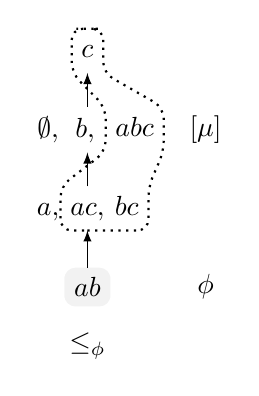
\begin{tikzpicture}
	%% total preorder
	\node at (0,-0.75){$\le_\phi$};
	
	\node at (0,0)(ab){$ab$};
	
	\node at (-0.5,1)(a){$\vphantom{b,}a,$};	
	\node at (0,1)(ac){$\vphantom{b}ac,$};
	\node at (0.5,1)(bc){$bc\vphantom{,}$};
	
	\node at (-0.5,2)(e){$\emptyset,$};
	\node at (0,2)(b){$b,\vphantom{\emptyset}$};
	\node at (0.6,2)(abc){$abc\vphantom{,}$};
	
	\node at (0,3)(c){$\vphantom{b,}c$};
	
	\node at (1.5,0){$\mods{\phi}$};
	\node at (1.5,2){$[\mu]$};
	
	\path[-latex] (ab)edge(ac)(ac)edge(b)(b)edge(c);
	
	\fill[opacity=0.05, rounded corners = 4]
		(ab.south)--
		(ab.south east)--
		(ab.east)--
		(ab.north east)--
		(ab.north)--
		(ab.north west)--
		(ab.west)--
		(ab.south west)--
		(ab.south);
	
	\draw[thick, dotted, rounded corners=4]
		(ac.south)--
		(bc.south)--
		(bc.south east)--
		(bc.east)--
		(bc.north east)--
		(abc.south east)--
		(abc.east)--
		(abc.north east)--
		(c.south east)--
		(c.east)--
		(c.north east)--
		(c.north)--
		(c.north west)--
		(c.west)--
		(c.south west)--
		(abc.north west)--
		(abc.west)--
		(abc.south west)--
		(ac.north west)--
		(ac.west)--
		(ac.south west)--
		(ac.south);
	\end{tikzpicture}
	\caption{
		Total preorder $\le_\phi$, for $[\phi]=\{ab\}$.
		Lower interpretations are better.
		The new information is $\mu = c$,
		and its models are surrounded by the dotted line.
		Revising $\phi$ by $\mu$ amounts to selecting the 
		$\le_\phi$-minimal models of $\mu$.
	}
	\label{fig:3-revision-preorder-operator-interplay}
\end{figure}

\begin{xmpl}{A monopoly on tool use after all?}{3-revision-preorder-operator-interplay}
	We revisit our running revision scenario,
	detailed in 
	Examples \ref{ex:1-revision-motivation}, 
	\ref{ex:3-revision-basic-setup} and \ref{ex:3-revision-R1,3,4}
	with Jane Goodall challenging the primatology status quo.
	This status quo is
	expressed as the propositional formula $\phi$,
	with $[\phi]=\{ab\}$,
	while Jane Goodall's challenge to it
	is the finding $\mu$, with $[\mu]=\{c,ac,bc,abc\}$.
	Suppose that revision among the primatology community 
	is guided by a total r-faithful assignment $\as$
	that assigns to $\phi$ the
	total preorder $\le_\phi$ on interpretations 
	in Figure \ref{fig:3-revision-preorder-operator-interplay}.
	According to the preorder $\le_{\P}$, the state of the world 
	$ab$ is the most likely outcome: this corresponds
	with $ab$ being the unique model of the prior belief $\phi$,
	and is in agreement with properties $\oor{5-7}$.
	Jane Goodall's finding reveals that the only 
	viable outcomes are those consistent with $\mu$
	i.e., the models of $\mu$,
	and that a choice must be made as to which of these model
	will go into the new belief.
	How does the choice take place?
	We have that 
	$[\phi\re^\as\mu] = \min_{\le_\phi}[\mu] = \{ac,bc\}$,
	or, to put it differently,
	$\phi\re^\as\mu\equiv (a\land\lnot b\land c)\lor (\lnot a\land b\land c)$.
	That is, according to $\le_\phi$, the most plausible 
	states of affairs consistent with $\mu$, 
	i.e., the $\le_\phi$-minimal models of $\mu$,
	are $ac$ and $bc$,
	and the rational course of action is to adopt 
	them as the new belief.

	Recall, as well, Louis Leakey's telegram to Jane Goodall
	from Example \ref{ex:1-revision-motivation}:
	``Now we must redefine tool, redefine Man, or accept chimpanzees as humans.''
	Given how we model the problem, 
	Leakey seems to think that the result of revising by $\mu$
	should be either $bc$, 
	i.e., chimpanzees use tools and are not human, 
	but humans don't use tool (redefining tool),
	or $ac$, i.e., chimpanzees and humans use tools, 
	but chimpanzees are human (accepting chimpanzees as humans).
	If we assume that Louis Leakey had the same prior belief $\phi$
	as the rest of the primatology community
	but was revising according to a revision operator $\re^{LL}$,
	then his telegram seems to suggest an inclination to 
	conclude that $ac$ or $bc$ must be the case.
	In other words, narrowing down the choice to only these two outcomes 
	(i.e., to $\px_{ac,bc}\equiv c \land (a\leftrightarrow\lnot b)$),
	then Leakey seems to think that they cannot be distinguished,
	i.e., $[\phi\re^{LL}\px_{ac,bc}]=\{ac,bc\}$.
	In the exhaustive revealed ranking we would then infer 
	that, for Leakey, it holds that $ac\approx^\exh_\phi bc$,
	and the preorder $\le_\phi$ 
	in Figure \ref{fig:3-revision-preorder-operator-interplay}
	is consistent with this attitude,
	whereas in the exclusive revealed ranking we 
	would infer that $ac\not\le^\exc_\phi bc$ 
	and $ac\not\le^\exc_\phi bc$. 
\end{xmpl}

Example \ref{ex:3-revision-preorder-operator-interplay} illustrates
that rankings of outcomes tell us something,
not about the state of the world,
but about what an agent thinks is more likely.
They can be used to guide revision,
or, conversely, they can be reconstructed, piece by piece,
from putative revision behavior.
But what ensures that a revision operator guided by a plausibility
ranking on outcomes is rational?
And how can we guarantee that the revealed rankings add up to 
a coherent whole?
The answer depends entirely on the constraints imposed on the revision 
operator and on the plausibility rankings,
with the representation results below showing that there is 
a close link between the revision postulates $\ppr{1-8}$
and properties $\oor{1-7}$.
The first result shows that leaving out postulate $\ppr{2}$
and enforcing postulate $\ppr{6}$
results in revision policies that are represented 
by total assignments on interpretations that are also insensitive to syntax,
which, we recall, means that $\le_\phi$ satisfies properties $\oor{1-4}$
(i.e., is a total preorder on $\U$),
and that
$[\phi\re\mu]=\min_{\le_\phi}[\mu]$,
for any propositional formulas $\phi$ and $\mu$.
Recall, as well, that the $\L$-proxy of a set $\{w_1,\dots,w_k\}$ of interpretations
is a propositional formula $\px_{1,\dots,k}$ such that 
$[\px_{1,\dots,k}]=\{w_1,\dots,w_k\}$.

\begin{thm}{}{3-revision-repr-total}
	A revision operator $\re$ satisfies postulates 
	$\ppr{1}$ and $\ppr{3-6}$ (i.e., is exhaustive)
	if and only if there exists	an 
	$\L$-assignment $\as$ on interpretations
	that satisfies properties $\oor{1-4}$
	(i.e., is total and insensitive to syntax)
	and represents the operator $\re$.
\end{thm}
\begin{prf*}{}{}%{}{}
	(``$\Leftarrow$'')
	Assume, first, that we are given an $\L$-assignment $\as$ on interpretations
	such that, for any $\phi\in\L$,	$\le_\phi$ satisfies properties $\oor{1-4}$.
	Since the $\as$-induced revision operator $\re^\as$ is
	defined by taking $[\phi\re^\as\mu]\defeq\min_{\le_\phi}[\mu]$, 
	the proof amounts to showing that $\re^\as$ satisfies postulates $\ppr{1-4}$.
	
	Postulate $\ppr{1}$ follows from the fact that 
	$\phi\re^\as\mu$ is a formula whose set of models is, by definition,
	a subset of $[\mu]$. Since $[\mu]$ is a finite set and, by properties $\oor{1-2}$,
	$\le_\phi$ is a pre-order, we then have 
	that $\min_{\le_\phi}[\mu]\neq\emptyset$, if $[\mu]\neq\emptyset$.
	This implies that postulate $\ppr{3}$ is satisfied.
	For postulate $\ppr{4}$ we have that if 
	$\phi_1\equiv\phi_2$, then, by property $\oor{4}$, 
	$\le_{\phi_1}=\le_{\phi_2}$.
	Clearly, then, if we also have that $\mu_1\equiv\mu_2$, 
	then it holds that $\min_{\le_{\phi_1}}[\mu_1]=\min_{\le_{\phi_2}}[\mu_2]$. 
	
	For postulate $\ppr{5}$, take $w_1\in[(\phi\re^\as\mu_1)\land\mu_2]$: this means that 
	$w_1\in\min_{\le_\phi}[\mu_1]\cap[\mu_2]$, and we want to show that 
	$w_1\in\min_{\le_\phi}[\mu_1\land\mu_2]$.
	Suppose, on the contrary, that $w_1\notin\min_{\le_\phi}[\mu_1\land\mu_2]$.
	Since we can derive, from our starting assumption, that $w_1\in[\mu_1\land\mu_2]$,
	it follows that $[\mu_1\land\mu_2]\neq\emptyset$,
	and hence that $\min_{\le_\phi}[\mu_1\land\mu_2]\neq\emptyset$.
	Thus there exists $w_2\in\min_{\le_\phi}[\mu_1\land\mu_2]$;
	since $w_1\notin\min_{\le_\phi}[\mu_1\land\mu_2]$
	we then conclude that $w_2<_\phi w_1$.
	But $w_1$ and $w_2$ are both in $[\mu_1]$ and $w_1\in\min_{\le_\phi}[\mu_1]$,
	which implies that $w_1\le_\phi w_2$. We have arrived at a contradiction,
	and thus $w_1\in\min_{\le_\phi}[\mu_1\land\mu_2]$.
	
	For postulate $\ppr6$, take $w_1\in\min_{\le_\phi}[\phi\re^\as(\mu_1\land\mu_2)]$.
	We want to show that $w_1\in[(\phi\re^\as\mu_1)\land\mu_2]$.
	From the fact that $w_1\in\min_{\le_\phi}[\phi\re^\as(\mu_1\land\mu_2)]$
	we infer that $w_1\in[\mu_2]$,
	so all we have to show is that $w_1\in[\phi\re^\as\mu_1]$.
	Suppose, on the contrary, that $w_1\notin[\phi\re^\as\mu_1]$:
	we now use the assumption that $(\phi\re^\as\mu_1)\land\mu_2$ is consistent 
	to conclude that there exists $w_2\in[(\phi\re^\as\mu_1)\land\mu_2]$,
	which implies that $w_2<_\phi w_1$.
	But, since $w_1\in\min_{\le_\phi}[\phi\re^\as(\mu_1\land\mu_2)]$
	and $w_2\in[\mu_1\land\mu_2]$, it also follows that $w_1\le_\phi w_2$.
	This is a contradiction, and we conclude that $w_1\in[\phi\re^\as\mu_1]$.
	
	(``$\Rightarrow$'')
	Assume, now, that we are given an exhaustive belief change operator $\re$, 
	i.e., one that satisfies postulates $\ppr{1}$ and $\ppr{3-6}$.
	We will show that the exhaustive $\re$-revealed assignment $\as^\exh$ 
	is the assignment we are looking for,
	i.e., $\le^\exh_\phi$ satisfies properties $\oor{1-4}$, for any propositional formula $\phi$,
	and $[\phi\re\mu]=\min_{\le^\exh_\phi}[\mu]$, for any propositional formula $\mu$.
	
	For property $\oor{1}$ (reflexivity), take an interpretation $w$ and 
	the $\L$-proxy $\px_w$ of $w$, i.e., a propositional formula such that $[\px_w]=\{w\}$.
	Notice that, using postulates $\ppr{1}$ and $\ppr{3}$, we can conclude that 
	$[\phi\re\px_w]=\{w\}$. This implies that $w\le^\exh_\phi w$.
	
	For property $\oor{2}$ (transitivity), assume there are interpretations $w_1$, $w_2$
	and $w_3$ such that $w_1\le^\exh_\phi w_2$ and $w_2\le^\exh_\phi w_3$. We want to show that $w_1\le^\exh_\phi w_3$.
	We will do this in two steps. 
	The first step consists in showing that $w_1\in[\phi\re\px_{1,2,3}]$,
	where $\px_{1,2,3}$ is an $\L$-proxy of $\{w_1,w_2,w_3\}$,
	i.e., a propositional formula such that $[\px_{1,2,3}]=\{w_1,w_2,w_3\}$. 
	First, notice that, by postulates $\ppr{1}$ and $\ppr{3}$, we have that 
	$\emptyset\subset[\phi\re\px_{1,2,3}]\subseteq[\px_{1,2,3}]$.
	In other words, $[\phi\re\px_{1,2,3}]$ contains at least one of the interpretations $w_1$,
	$w_2$ and $w_3$. We will do a case analysis to show that $w_1\in[\phi\re\px_{1,2,3}]$.
	
	\emph{Case 1}. If $w_1\in[\phi\re\px_{1,2,3}]$, the conclusion is immediate.
	
	\emph{Case 2}. If $w_2\in[\phi\re\px_{1,2,3}]$, then $(\phi\re\px_{1,2,3})\land\px_{1,2}$ is consistent.
	Using postulates $\ppr{5-6}$ and $\ppr{4}$,
	and keeping in mind that $\px_{1,2,3}\land\px_{1,2}\equiv\px_{1,2}$,
	this implies that:
	\begin{align*}
		(\phi\re\px_{1,2,3})\land\px_{1,2} &\equiv\phi\re(\px_{1,2,3}\land\px_{1,2}) &(\text{by}~\ppr{5-6})\\
		 										     &\equiv\phi\re\px_{1,2}. 		                 &(\text{by}~\ppr{4})
	\end{align*}
	By hypothesis, it holds that $w_1\le^\exh_\phi w_2$, which,
	by the definition of the $\re$-revealed exhaustive ranking, 
	implies that $w_1\in[\phi\re\px_{1,2}]$.
	Using this with the equivalence just derived, we arrive at the conclusion that $w_1\in[\phi\re\px_{1,2,3}]$.
	
	\emph{Case 3}. If $w_3\in[\phi\re\px_{1,2,3}]$,
	we infer that $(\phi\re\px_{1,2,3})\land\px_{2,3}$ is consistent.	
	Using, again, postulates $\ppr{5-6}$ and $\ppr{4}$,
	and keeping in mind that $\px_{1,2,3}\land\px_{2,3}\equiv\px_{2,3}$,
	this implies that:
	\begin{align*}
		(\phi\re\px_{1,2,3})\land\px_{2,3} &\equiv\phi\re(\px_{1,2,3}\land\px_{2,3}) &(\text{by}~\ppr{5-6})\\
		 										     &\equiv\phi\re\px_{2,3}. 		                 &(\text{by}~\ppr{4})
	\end{align*}
	Since $w_2\in[\phi\re\px_{2,3}]$ (because $w_2\le^\exh_\phi w_3$),
	we get that $w_2\in[\phi\re\px_{1,2,3}]$.
	We can now reproduce the reasoning from Case 2 to conclude that $w_1\in[\phi\re\px_{1,2,3}]$.
	
	Rounding up the case analysis, we can conclude that $w_1\in[\phi\re\px_{1,2,3}]$.
	With this in hand, we infer that $(\phi\re\px_{1,2,3})\land\px_{1,3}$ is consistent, 
	and we can apply the same blend of postulates $\ppr{5-6}$ and $\ppr{4}$,
	keeping in mind that $\px_{1,2,3}\land\px_{1,3}\equiv\px_{1,3}$:
	\begin{align*}
		(\phi\re\px_{1,2,3})\land\px_{1,3} &\equiv\phi\re(\px_{1,2,3}\land\px_{1,3}) &(\text{by}~\ppr{5-6})\\
		 										     &\equiv\phi\re\px_{1,3}. 		                 &(\text{by}~\ppr{4})
	\end{align*}
	Since $w_1\in[\phi\re\px_{1,2,3}]$ and $w_1\in[\px_{1,3}]$,
	we conclude that $w_1\in[\phi\re\px_{1,3}]$.
	By the definition of $\le^\exh_\phi$, this implies that $w_1\le^\exh_\phi w_3$.
	
	Property $\oor{3}$ (totality) follows from the fact for any two interpretations $w_1$ and $w_2$,
	there exists an $\L$-proxy $\px_{1,2}$ of $\{w_1,w_2\}$,
	and postulate $\ppr{3}$ guarantees that at least one of $w_1$ and $w_2$ is in $[\phi\re\px_{1,2}]$.
	Property $\oor{4}$ follows by using postulate $\ppr{4}$, i.e., 
	the fact that the definition of $\le^{\exh}_\phi$ 
	is not sensitive in any way to the syntax of $\phi$.
	
	The last thing we have to show is that 
	the exhaustive $\re$-revealed assignments represents $\re$,
	i.e., that $[\phi\re\mu]=\min_{\le^\exh_\phi}[\mu]$, for any propositional formula $\mu$.
	We do this by showing the double inclusion. 
	
	(``$\subseteq$'') 
	Take, first, $w_1\in[\phi\re\mu]$,
	and some arbitrary interpretation $w_2\in[\mu]$.
	Applying postulates $\ppr{5}$ and $\ppr{4}$
	and keeping in mind that, because $[\px_{1,2}]\subseteq[\mu]$,
	it holds that $\mu\land\px_{1,2}\equiv\px_{1,2}$,
	we have that:
	\begin{align*}
		(\phi\re\mu)\land\px_{1,2} &\models\phi\re(\mu\land\px_{1,2})    &(\text{by}~\ppr{5})\\
		 										     &\equiv\phi\re\px_{1,2}. &(\text{by}~\ppr{4})
	\end{align*}
	Since $w_1\in[(\phi\re\mu)\land\px_{1,2}]$, it follows that
	$w_1\in[\phi\re(\mu\land\px_{1,2})]$
	and then that $w_1\in[\phi\re\px_{1,2}]$.
	Thus, $w_1\le^{\exh}_\phi w_2$ and, 
	keeping in mind that $w_2$ was arbitrarily chosen among the models of $\mu$,
	we obtain that $w_1\in\min_{\le^\exh_\phi}[\mu]$.
	
	(``$\supseteq$'') 
	Take, now, $w_1\in\min_{\le^\exh_\phi}[\mu]$.
	We want to show that $w_1\in[\phi\re\mu]$.
	Suppose, on the contrary, that $w_1\notin[\phi\re\mu]$.
	Since, due to our assumption, it follows that $\mu$ is consistent,
	we have, by postulate $\ppr{3}$, that there exists $w_2\in[\phi\re\mu]$.
	Using postulates $\ppr{4}$ and $\ppr{6}$, we have that: 
	\begin{align*}
		\phi\re\px_{1,2} &\equiv\phi\re(\mu\land\px_{1,2})    &(\text{by}~\ppr{4})\\
		 					  &\models(\phi\re\mu)\land\px_{1,2}. &(\text{by}~\ppr{6})
	\end{align*}
	By assumption, we have that $w_1\notin[\phi\re\mu]$, and from this it follows that 
	$w_1\notin[(\phi\re\mu)\land\px_{1,2}]$ and, using the implications just derived,
	it holds that
	$w_1\notin[\phi\re\px_{1,2}]$,
	and hence $w_2<^\exh_\phi w_1$.
	But we also have that $w_1\in\min_{\le^\exh_\phi}[\mu]$ and $w_2\in[\mu]$,
	which implies that $w_1\le^\exh_\phi w_2$.
	We have thus arrived at a contradiction.
\end{prf*}

% Theorem \ref{thm:3-revision-repr-total} says that an exhaustive revision operator $\re$
% (i.e., satisfying postulates $\ppr{1}$ and $\ppr{3-6}$)
% is represented by an assignment $\as$ mapping propositional formulas to total preorders, 
% such that $\re$ coincides with the operator induced by the exhaustive revealed assignment $\as^\exh$.
% Thus, one way of thinking of postulates $\ppr{1}$ and $\ppr{3-6}$ is that they axiomatize 
% a choice function on total preorders $\le_\phi$ on interpretations.
% The preorder $\le_\phi$ can be thought of as a plausibility ranking on
% interpretations and is biased towards the prior beliefs $\phi$, in the sense that 
% it ranks the models of $\phi$ as the most plausible interpretations:
% this is in accord with the intuition that a belief in $\phi$ means that states of affairs
% consistent with $\phi$ are thought to be the most likely candidates for the true state of the world.
% In this context, newly acquired information $\mu$ shifts this perspective
% by providing a different menu of states of affairs that are suitable for belief.
% The choice procedure, as traditionally construed, then forms a new belief by choosing among the models of $\mu$
% the most plausible interpretations according to $\le_\phi$.
% [[MORE on the connections to choice]]

The result of Theorem \ref{thm:3-revision-repr-total} is not exactly new, 
and can be easily extracted from the literature \cite{KatsunoM92};
it is certainly present in Hans Rott's work \cite{Rott01}.
Nonetheless, in many standard presentations 
postulates $\ppr{1}$ and $\ppr{3-6}$ are taken together 
with postulate $\ppr{2}$, creating the impression that the postulates
are inextricably tied together. 
Our purpose here is to separate the postulates
that guarantee the structural properties $\oor{1-3}$ 
of the assignment $\as$,
from the postulates that say where the 
models of $\phi$ should be placed in that preorder.
Theorem \ref{thm:3-revision-repr-total} 
allows us to see that these are two distinct issues.

The second result shows that leaving out postulate $\ppr{2}$ 
and enforcing postulates $\ppr{7-8}$ instead of $\ppr{6}$
results in revision policies that are represented by partial assignments on interpretations
that are also insensitive to syntax.
Recall, this means that $\le_\phi$ satisfies properties 
$\oor{1-2}$ (i.e., is a partial preorder on $\U$)
and $\oor{4}$, and that
$[\phi\re\mu]=\min_{\le_\phi}[\mu]$,
for any propositional formulas $\phi$ and $\mu$.

\begin{thm}{}{3-revision-repr-partial}
	A revision operator $\re$ satisfies postulates $\ppr{1}$, $\ppr{3-5}$ and $\ppr{7-8}$ 
	(i.e., is exclusive)
	if and only if there exists	
	an $\L$-assignment $\as$ on interpretations
	that satisfies properties $\oor{1-2}$ and $\oor{4}$
	(i.e., is partial and insensitive to syntax) 
	and represents the operator $\re$.
\end{thm}
\begin{prf*}{}{}%
	(``$\Leftarrow$'')
	Starting from an $\L$-assignment $\as$ on interpretations
	that satisfies properties $\oor{1-2}$ and $\oor{4}$,
	the argument that $\re^\as$ satisfies postulates $\ppr{1}$ and $\ppr{3-5}$ is entirely similar
	to the argument for Theorem \ref{thm:3-revision-repr-total}.
	
	For postulate $\ppr{7}$, we have to show that 
	$\min_{\le_\phi}[\mu_1]=\min_{\le_\phi}[\mu_2]$.
	Take, then, $w_1\in\min_{\le_\phi}[\mu_1]$ and suppose that $w_1\notin\min_{\le_\phi}[\mu_2]$.
	By postulate $\ppr{3}$ we have that $\phi\re^\as\mu_2$ is consistent, 
	which implies that there exists $w_2\in\min_{\le_\phi}[\mu_2]$ such that 
	$w_2<_\phi w_1$.
	By the assumption of $\ppr{7}$, it holds that $\phi\re^\as\mu_2\models\mu_1$,
	from which it follows that $w_2\in[\mu_1]$
	and, since $w_1\in\min_{\le_\phi}[\mu_1]$, it follows that $w_2\not<_\phi w_1$,
	We have arrived, in this way, at a contradiction, and thus we conclude
	that $\phi\re^\as\mu_1\models\phi\re^\as\mu_2$.
	The argument that $\phi\re^\as\mu_2\models\phi\re^\as\mu_1$ is entirely similar.
	Together, these two facts imply that $\phi\re^\as\mu_1\equiv\phi\re^\as\mu_2$.
	
	For postulate $\ppr{8}$, take $w\in\min_{\le_\phi}[\mu_1]\cap\min_{\le_\phi}[\mu_2]$ 
	and suppose that $w\notin\min_{\le_\phi}[\mu_1\lor\mu_2]$.
	By postulate $\ppr{3}$ we have that $\min_{\le_\phi}[\mu_1\lor\mu_2]\neq\emptyset$,
	and thus there exists $w'\in\min_{\le_\phi}[\mu_1\lor\mu_2]$ such that 
	$w'<_\phi w$. Since, by postulate $\ppr{1}$, it holds that $w'\in[\mu_1\lor\mu_2]$,
	we conclude that $w'$ has to be an element of $[\mu_1]$ or of $[\mu_2]$.
	This leads to a contradiction with the fact that $w\in\min_{\le_\phi}[\mu_1]\cap\min_{\le_\phi}[\mu_2]$,
	because from this we are forced to conclude that $w'\not<_\phi w$.
	
	(``$\Rightarrow$'')
	Given a revision operator $\re$ that satisfies postulates $\ppr{1}$, $\ppr{3-5}$ and $\ppr{7-8}$,
	we will show that the exclusive $\re$-induced $\L$-assignment $\as^\exc$ on interpretations 
	is the assignment we are looking for, 
	i.e., $\le^\exc_\phi$ satisfies properties $\oor{1-2}$ and $\oor{4}$, 
	for any propositional formula $\phi$ and, for any 
	propositional formula $\mu$, 
	it holds that $[\phi\re\mu]=\min_{\le^\exc_\phi}[\mu]$. 

	For $\oor{1}$ (reflexivity), note that, by postulates $\ppr{1}$ and $\ppr{3}$,
	it holds, for any interpretation $w$, that $[\phi\re\px_w]=\{w\}$.
	This implies that $w\le^\exc_\phi w$.
	
	To show that $\le^\exc$ satisfies property $\oor{3}$ (i.e., is transitive),
	take interpretations $w_1$, $w_2$ and $w_3$ such that 
	$w_1$, $w_2$ and $w_3$ are pairwise distinct and
	$w_1\le^\exc_\phi w_2$ and $w_2\le^\exc_\phi w_3$. 
	We show, first, that $[\phi\re\px_{1,2,3}]=\{w_1\}$,
	where $\px_{1,2,3}$ is an $\L$-proxy of the set $\{w_1, w_2,w_3\}$,
	i.e., a propositional formula such that $[\px_{1,2,3}]=\{w_1,w_2,w_3\}$.
	To that end, note that, by postulates $\ppr{1}$ and $\ppr{3}$, we have that
	$\emptyset\subset[\phi\re\px_{1,2,3}]\subseteq[\px_{1,2,3}]$.
	Suppose, now, that $w_2\in[\phi\re\px_{1,2,3}]$.
	This means that $w_2\in[(\phi\re\px_{1,2,3})\land\px_{1,2}]$.
	Applying postulates $\ppr{5}$ and $\ppr{4}$ we obtain that:
	\begin{align*}
		(\phi\re\px_{1,2,3})\land\px_{1,2} &\models\phi\re (\px_{1,2,3}\land\px_{1,2}) &(\text{by}~\ppr{5})\\
													 &\equiv\phi\re\px_{1,2}.                        &(\text{by}~\ppr{4}) 
	\end{align*}
	But this implies that $w_2\in[\phi\re\px_{1,2}]$, which is a contradiction,
	since, by hopthesis we have that $w_1\le^\exc_\phi w_2$, which, by the definition of $\le^\exc_\phi$,
	implies that $[\phi\re\px_{1,2}]=\{w_1\}$.
	This shows that $w_2\notin[\phi\re\px_{1,2,3}]$. 
	Applying the same strategy to $[(\phi\re\px_{1,2,3})\land\px_{2,3}]$,
	it follows that $w_3\notin[\phi\re\px_{1,2,3}]$.
	Thus, the only remaining possibility is that $[\phi\re\px_{1,2,3}]=\{w_1\}$.

	With this result in hand, we have that $\phi\re\px_{1,2,3}\models\px_{1,3}$.
	It is straightforward to see that $\phi\re\px_{1,3}\models\px_{1,2,3}$,
	which allows us to apply postulate $\ppr{7}$ and infer that $\phi\re\px_{1,2,3}\equiv\phi\re\px_{1,3}$.
	This means that $[\phi\re\px_{1,3}]=\{w_1\}$ and, by the definition of $\le^\exc_\phi$,
	it follows that $w_1\le^\exc_\phi w_3$.

	For $\oor{4}$ (i.e., insensitivity to the syntax of $\phi$ and $\mu$), the argument is entirely similar 
	to the one given in the proof of Theorem \ref{thm:3-revision-repr-total}.

	Finally, we show that $[\phi\re\mu]=\min_{\le^\exc_\phi}[\mu]$ by double inclusion.

	(``$\subseteq$'') 
	Take, first, $w\in[\phi\re\mu]$ and suppose $w\notin\min_{\le^\exc_\phi}[\mu]$.
	This means that there exists $w'\in\min_{\le^\exc_\phi}[\mu]$ such that $w'<^\exc_\phi w$,
	which in turn implies that $[\phi\re\px_{w,w'}]=\{w'\}$.
	But, by postulates $\ppr{5}$ and $\ppr{4}$, we have that:
	\begin{align*}
		(\phi\re\mu)\land\px_{w,w'} & \models\phi\re(\mu\land\px_{w,w'}) &(\text{by}~\ppr{5})\\
										 & \equiv\phi\re\px_{w,w'}.		   &(\text{by}~\ppr{4})
	\end{align*}
	Thus, since $w\notin[\phi\re\px_{w,w'}]$ but $w\in[\px_{w,w'}]$, it follows that $w\notin[\phi\re\mu]$,
	which is a contradiction.

	(``$\supseteq$'') 
	Take, now, $w\in\min_{\le^\exc_\phi}[\mu]$ and suppose $w\notin[\phi\re\mu]$,
	and an arbitrary $w_i\in[\mu]$. Since $w\in\min_{\le^\exc_\phi}[\mu]$,
	it cannot be the case that $w_i<^\exc_\phi w$, which implies that 
	$w\in[\phi\re\px_{w,w_i}]$:
	to see why, suppose that $w\notin[\phi\re\px_{w,w_i}]$;
	by postulates $\ppr{1}$ and $\ppr{3}$, $[\phi\re\px_{w,w_i}]$ 
	needs to be a non-empty subset 
	of $[\px_{w,w_i}]$, 
	and this implies that $[\phi\re\px_{w,w_i}]=\{w_i\}$,
	hence $w_i<^{\exc}_{\phi}w$.
	Applying postulate $\ppr{8}$ for every $w_i\in[\mu]$, 
	and keeping in mind that $\bigvee_{w_i\in[\mu]}\px_{w,w_i}\equiv\mu$,
	we obtain that:
	\begin{align*}
		\bigwedge_{w_i\in[\mu]}(\phi\re\px_{w,w_i}) 		& 
		\models\phi\re(\bigvee_{w_i\in[\mu]}\px_{w,w_i}) 	&
		(\text{by}~\ppr{5})										\\
																& 
		\equiv\phi\re\mu.                                       &
		(\text{by}~\ppr{4})										\\ 
	\end{align*}
	It then follows that $w\in[\phi\re\mu]$.
\end{prf*}

Theorems \ref{thm:3-revision-repr-total} and \ref{thm:3-revision-repr-partial}
make it official:
the behavior of an agent revising its beliefs according to postulates $\ppr{1}$, $\ppr{3-5}$
and either postulate $\ppr{6}$ or postulates $\ppr{7-8}$,
can be rationalized using preorders on outcomes, such that the outcomes the agent 
ends up accepting as part of its revised belief are the most plausible outcomes
consistent with the new information.
It is as if the new information provides a menu of allowable alternatives, 
and the agent chooses the best outcomes from this menu to believe.

Indeed, the similarity of this perspective with the rational choice framework for a single agent
presented in Section \ref{sec:2-choice-functions} runs deeper,
as an $\L$-revision operator $\re$ can be seen to be a choice function
over the set $\U$ of interpretations, 
with $[\mu]$ as the choice set.
Contemplation of postulates $\ppr{1}$, $\ppr{3}$ and $\ppr{5-6}$ quickly reveals 
the parallel to the axioms for choice functions:
viewed semantically, postulates $\ppr{1}$ and $\ppr{3}$ say that 
$[\phi\re\mu]\subseteq[\mu]$ and that, if $[\mu]\neq\emptyset$, 
then $[\phi\re\mu]\neq\emptyset$,
which coincides with properties $\ooch{1}$ and $\ooch{2}$, 
respectively, of a choice function.
Since these properties can be taken to be constitutive of a 
choice function, we could even prove a mini-result saying that any 
revision operator satisfying postulates $\ppr{1}$ and $\ppr{3-4}$
is equivalent to a choice function on the set $\U$ of interpretations
satisfying properties $\ooch{1-2}$: this is sufficiently obvious, however,
to leave it as an observation.

Moving further, it can be seen that postulates $\ppr{5}$ and $\ppr{6}$ 
coincide with properties $\ooch{3}$ and $\ooch{5}$, respectively.
Correspondingly, deviations from them are similar in spirit:
Examples \ref{ex:3-revision-R5,6} and \ref{ex:3-revision-R8},
showing agents that revise in ways inconsistent with postulates $\ppr{5-8}$
are, on a close reading, entirely consonant with Example \ref{ex:2-choice-props},
showing an agent that chooses in ways inconsistent with properties $\ooch{3-4}$.
The parallel is entirely justified, as both types of agents exhibit 
the same kind of pathological behavior when choosing among a set menu:
the doctors in Examples \ref{ex:3-revision-R5,6} and \ref{ex:3-revision-R8} are just choosing 
odd things to believe, or, to be more precise, they revise in ways that are not 
immediately rationalizable by unique plausibility relations on outcomes.
In the same spirit, Theorem \ref{thm:3-revision-repr-total} can be seen 
as a direct analogue of Theorem \ref{thm:2-choice-repr}.
Postulate $\ppr{4}$ has no analogue in the choice framework, since no distinction 
is made there between syntax and semantics.

We can see unfolding here 
a point that has been made before in belief change
\cite{Rott92,Schulte99,Rott01,Bonanno09,Arlo-CostaP10}, 
namely that the choice perspective 
is integral to the workings of a revision operator.
And, while we will want to take up this point and explore it further,
it is important to not be too carried away by its significance.
We certainly do not want to suggest that either 
properties $\ooch{1-5}$ or postulates $\ppr{1}$ and $\ppr{3-8}$
uniquely characterize rational choice or rational belief change,
since examples to the contrary are readily available 
\cite{Sen77,Olsson03,Kahneman11}: rationality, as we have mentioned before, 
comes in many flavors, and what is rational in one type of situation 
may not be rational in another.
We can thus presume that the properties covered
so far in Section \ref{sec:2-choice-functions} and in the present section 
touch on only a very small part of 
the whole gamut of rational behavior,
and, inde. 
So, while, we do not want to give this particular formulation 
undue weight, we do want to use the broader implication, 
i.e., that belief change is a type of change, 
to explore the variety of change procedures 
that could count as rational.

Along these lines, we can start thinking of the role of postulate $\ppr{2}$
in the lineup of desirable revision postulates.
One thing that emerges from
Theorems \ref{thm:3-revision-repr-total} and \ref{thm:3-revision-repr-partial} 
is that postulates $\ppr{1}$ and $\ppr{3-5}$,
together with either postulate $\ppr{6}$ or postulates $\ppr{7-8}$,
regulate only the structural properties of the preorder $\le_{\phi}$ 
in an assignment, 
and say nothing about how the prior information $\phi$ 
biases $\le_{\phi}$, 
i.e., about the position of the models of $\phi$ in $\le_\phi$.
This latter aspect, as we will see in Theorems \ref{thm:3-revision-repr-R2-total}
and \ref{thm:3-revision-repr-R2-partial}, 
is traditionally enforced through postulate $\ppr{2}$.
For these results keep in mind 
that an $\L$-proxy of a pair 
$\{w_1,w_2\}$ of interpretations is a propositional formula $\px_{1,2}$ 
such that $[\px_{1,2}]=\{w_1,w_2\}$,
and that the lessons of 
Theorems \ref{thm:3-revision-repr-total} and \ref{thm:3-revision-repr-partial}
are that exhaustive and exclusive $\L$-revision operators 
are guaranteed to be represented by total and partial $\L$-assignments 
on interpretations, respectively.

\begin{thm}{}{3-revision-repr-R2-total}
	If a revision operator $\re$ satisfies postulates 
	$\ppr{1}$ and $\ppr{3-6}$ (i.e., is exhaustive)
	and $\as$ is an
	$\L$-assignment on interpretations that
	satisfies properties $\oor{1-4}$ (i.e., is total and syntax insensitive) 
	and represents the operator $\re$,
	then 
	$\re$ satisfies postulate $\ppr{2}$ if and only if
	$\as$ satisfies properties $\oor{5-7}$
	(i.e., is r-faithful).
\end{thm}
\begin{prf*}{}{}%
	(``$\Rightarrow$'')
	We start with a revision operator $\re$ satisfies postulates 
	$\ppr{1}$ and $\ppr{3-6}$ and a total, syntax insensitive 
	$\L$-assignment $\as$ on interpretations
	that represents it. 
	Consider, now, a propositional formula $\phi$ and 
	two interpretations $w_1$ and $w_2$ such that 
	$w_1$ and $w_2$ are models of $\phi$.
	Using postulate $\ppr{2}$, we can conclude that $[\phi\re\px_{1,2}]=\{w_1,w_2\}$,
	which, together with the fact that $\le_{\phi}$ is total, 
	implies that $w_1\approx_{\phi} w_2$,
	showing that property $\oor{5}$ is satisfied.
	If $w_1\in[\phi]$ and $w_2\notin[\phi]$, then with postulate $\ppr{2}$ again 
	we conclude that $[\phi\re\px_{1,2}]=\{w_1\}$,
	which implies that $w_1<_{\phi}w_2$, showing that property $\oor{7}$ is satisfied.

	(``$\Leftarrow$'')
	Conversely, we have to show that if $[\phi\land\mu]\neq\emptyset$,
	then $\min_{\le_{\phi}}[\mu]=[\phi\land\mu]$. We can do this by showing the 
	double inclusion.

	(``$\subseteq$'')
	Take $w_1\in\min_{\le_{\phi}}[\mu]$ and suppose $w_1\notin[\phi\land\mu]$.
	Since $w_1\in[\mu]$, by postulate $\ppr{1}$,
	the latter fact implies that $w_1\notin[\phi]$.
	Since $[\phi\land\mu]\neq\emptyset$, there exists an 
	interpretation $w_2\in[\phi\land\mu]$.
	We infer from this that $w_2\in[\phi]$ and, together with property $\oor{7}$,
	that $w_2<_{\phi}w_1$.
	But $w_1\in\min_{\le_{\phi}}[\mu]$, so this creates a contradiction.

	(``$\supseteq$'')
	Take $w_1\in[\phi\land\mu]$ and an arbitrary interpretation $w_2\in[\mu]$.
	Using properties $\oor{5}$ and $\oor{7}$, and keeping in mind that 
	$\le_{\phi}$ is total, we conclude that $w_1 \le_{\phi}w_2$,
	which implies that $w_1\in\min_{\le_{\phi}}[\mu]$.
\end{prf*}

Theorem \ref{thm:3-revision-repr-R2-total} takes care of the case 
when $\re$ satisfies the stronger postulate $\ppr{6}$ and is represented 
by a total assignment.
We can obtain a similar result for the case when $\re$ satisfies the weaker postulates 
$\ppr{7-8}$ instead of $\ppr{6}$, and is represented by a partial assignment.

\begin{thm}{}{3-revision-repr-R2-partial}
	If a revision operator $\re$ satisfies postulates 
	$\ppr{1}$, $\ppr{3-5}$ and $\ppr{7-8}$ (i.e., is exclusive)
	and $\as$ is an
	$\L$-assignment on interpretations that
	satisfies properties $\oor{1-2}$ and $\oor{4}$ 
	(i.e., is partial and syntax insensitive) 
	and represents the operator $\re$,
	then 
	$\re$ satisfies postulate $\ppr{2}$ if and only if
	$\as$ satisfies properties $\oor{6}$ and $\oor{7}$
	(i.e., is r-faithful).
\end{thm}
\begin{prf*}{}{}%
	The proof here follows the same lines as the proof for 
	Theorem \ref{thm:3-revision-repr-R2-total},
	so more intuitions can be gleaned from there.

	(``$\Rightarrow$'')
	If $w_1,w_2\in[\phi]$,
	then using postulate $\ppr{2}$ gives us that $[\phi\re\px_{1,2}]=\{w_1,w_2\}$.
	However, since $\le_{\phi}$ is not guaranteed to be total, we cannot conclude 
	that $w_1\approx_{\phi}w_2$; however, we can conclude that $w_1\not<_{\phi}w_2$
	and $w_2\not<_{\phi}w_1$, which means that property $\oor{6}$ is satisfied.
	If $w_1\in[\phi]$ and $w_2\notin[\phi]$, we obtain using postulate $\ppr{2}$ that 
	$[\phi\re\px_{1,2}]=\{w_1\}$, which implies that $w_1<_{\phi}w_2$, 
	showing that property $\oor{7}$ is satisfied.

	(``$\Leftarrow$'')
	We have to show that if $[\phi\land\mu]\neq\emptyset$,
	then $\min_{\le_{\phi}}[\mu]=[\phi\land\mu]$.
	The proof that $\min_{\le_{\phi}}[\mu]\subseteq[\phi\land\mu]$ 
	is entirely similar as for Theorem \ref{thm:3-revision-repr-R2-total}.
	To show that $[\phi\land\mu]\subseteq\min_{\le_{\phi}}[\mu]$,
	suppose that there exists an interpretation $w_1\in[\phi\land\mu]$
	such that $w_1\notin\min_{\le_{\phi}}[\mu]$.
	This means that there exists $w_2\in\min_{\le_{\phi}}[\mu]$
	such that $w_2<_{\phi}w_1$.
	Using the previous result, we can conclude that $w_2\in[\phi]$.
	Since $w_1\in[\phi]$, this contradicts property $\oor{6}$.
\end{prf*}

Theorems \ref{thm:3-revision-repr-total} and \ref{thm:3-revision-repr-R2-total} 
add the final touches to a variant of revision that makes up the 
standard, received Katsuno-Mendelzon model.
Stitching them together with 
Theorems \ref{thm:3-revision-repr-partial} and \ref{thm:3-revision-repr-R2-partial}
gives us the classical  representation results found in the literature,
the first of which is for total preorders.

\begin{thm}{\cite{KatsunoM92}}{3-revision-repr-km-total}
	A revision operator $\re$ satisfies postulates $\ppr{1-6}$ 
	if and only if
	there exists an $\L$-assignment $\as$ on interpretations
	that satisfies properties $\oor{1-7}$
	(i.e., that is total, syntax insensitive and r-faithful) 
	and that represents the operator $\re$.
\end{thm}

The assignment representing an exhaustive operator $\re$, we know from 
Theorems \ref{thm:3-revision-repr-total},
is the exhaustive $\re$-revealed assignment $\as^{\exh}$,
based on pairwise comparisons of interpretations.
The second result is for partial preorders.

\begin{thm}{\cite{KatsunoM92}}{3-revision-repr-km-partial}
	A revision operator $\re$ satisfies postulates $\ppr{1-5}$ and $\ppr{7-8}$ 
	if and only if
	there exists an $\L$-assignment $\as$ on interpretations
	that satisfies properties $\oor{1-2}$, $\oor{4}$ and $\oor{6-7}$
	(i.e., that is partial, syntax insensitive and r-faithful)
	and that represents the operator $\re$.
\end{thm}

In this case, the assignment representing $\re$ is the exclusive $\re$-revealed assignment.
Theorems \ref{thm:3-revision-repr-km-total} and \ref{thm:3-revision-repr-km-partial} 
gather together the insights of the Katsuno-Mendelzon model:
revision according to the postulates given in this section, 
in either of the variants considered, 
amounts to choosing the best outcomes available, 
according to a ranking on outcomes
that is biased by the agent's belief.

But where do such rankings come from?

\subsubsection{Distance-based revision operators}
In Section \ref{sec:2-distances} we presented a 
general method for computing distances from a propositional
formula $\phi$ to an interpretation $w$,
using two ingredients:
the first is a quasi-distance function $\dd$ between interpretations,
used to generate a tuple $(\dd(v,w))_{v\in[\phi]}$ of distances 
between every model of $\phi$ and $w$,
while the second ingredient is an aggregation function $\agg$ used to
aggregate the values in the tuple $(\dd(v,w))_{v\in[\phi]}$
and generate the $(\dd,\:\agg)$-induced distance 
$\dd^{\agg}(\phi,w)$ from $\phi$ to $w$. 
In this section we want to use this notions to 
rank interpretations relative to a formula $\phi$.
Thus, if $\dd$ is a quasi-distance between interpretations,
$\agg$ is an aggregation function,
$\phi$ is a propositional formula,
the \emph{$(\dd,\:\agg)$-induced ranking $\le^{\dd,\:\agg}_{\phi}$}
is defined,
for any two interpretations $w_1$, $w_2$,
as follows:
$$
	w_1 \le^{\dd,\:\agg}_{\phi}w_2~\text{if}~\dd^{\agg}(\phi,w_1)\le \dd^{\agg}(\phi,w_2).
$$
Intuitively, $w_1$ is considered better than $w_2$ according to $\le^{\dd,\:\agg}_{\phi}$
if $w_1$ is closer to $\phi$ than $w_2$, according to the measures uses.
For this section, where we are focused on techniques used in the existing literature,
we will assume that the aggregation function is $\min$ throughout.
Thus, to rephrase things,
if $\dd$ is a quasi-distance between interpretations,
the $(\dd,\:\min)$-induced ranking $\le^{\dd,\:\min}_{\phi}$ is obtained 
by taking, for any two interpretations $w_1$, $w_2$:
\begin{displaymath}
	w_1\le^{\dd,\:\min}_{\phi} w_2~\text{if}~\min(\dd(v,w_1))_{v\in[\phi]}\le\min(\dd(v,w_2))_{v\in[\phi]}.
\end{displaymath}
In other words, an agent whose prior belief is $\phi$ considers 
interpretation $w_1$ more plausible than $w_2$ 
if the shortest distance between $w_1$ and the models of $\phi$ 
is shorter than the shortest distance between $w_2$ and the models of $\phi$,
i.e., if $w_1$ is overall closer to the models of $\phi$ than $w_2$.
If $\dd$ is a quasi-distance,
the \emph{${(\dd,\:\min)}$-induced assignment $\as^{\dd,\:\min}$} is obtained by taking 
$\as^{\dd,\:\min}\!\!(\phi)=\le_\phi^{\dd,\:\min}$,
for any propositional formula $\phi$.
In the same vein, the \emph{${(\dd,\:\min)}$-induced revision operator $\re^{\dd,\:\min}$} 
is the operator induced by the assignment $\as^{\dd,\:\min}$.
This allows us to generate total, syntax insensitive r-faithful assignments.

\begin{prp}{}{3-revision-d-induced-preorder}
	If $\dd$ is a quasi-distance between interpretations and $\phi$ is a propositional formula, 
	the ${(\dd,\:\min)}$-induced ranking $\le^{\dd,\:\min}_\phi$ 
	satisfies properties $\oor{1-5}$ and $\oor{7}$,
	i.e., $\le^{\dd,\:\min}_\phi$ is total, syntax insensitive and r-faithful.
\end{prp}
\begin{prf*}{}{}%
	Since interpretations in $\le_{\phi}^{\dd,\:\min}$ are ranked based on the $\min$-aggregated distance
	from $\phi$, which in this case is a single number,
	it is straightforward to see that $\le_{\phi}^{\dd,\:\min}$ is a total preorder on interpretations,
	i.e., that $\le_{\phi}^{\dd,\:\min}$ satisfies properties $\oor{1-3}$.
	Since the definition of $\le_{\phi}^{\dd,\:\min}$ depends only on the interpretations,
	$\le_{\phi}^{\dd,\:\min}$ also satisfies property $\oor{4}$.
	Finally, it holds that 
	$\dd^\min(\phi,w) = \min(\dd(v,w))_{v\in[\phi]} = 0$ if and only if
	$w\in[\phi]$, 
	which implies that models of $\phi$ are the $\le_{\phi}^{\dd,\:\min}$-minimal
	elements in $\le_{\phi}^{\dd,\:\min}$,
	i.e., $\le_{\phi}^{\dd,\:\min}$ satisfies properties $\oor{5}$ and $\oor{7}$, for any propositional formula $\phi$.		
\end{prf*}

Proposition \ref{prop:3-revision-d-induced-preorder} 
implies that the $({\dd,\:\min})$-induced assignment $\as^{\dd,\:\min}$ 
is total, r-faithful and syntax insensitive, 
which, by Theorem \ref{thm:3-revision-repr-km-total}, 
implies that the $({\dd,\:\min})$-induced revision operator 
$\re^{\dd,\:\min}$ satisfies postulates $\ppr{1-6}$.

\begin{crl}{}{3-revision-d-induced-operator}
	If $\dd$ is a quasi-distance between interpretations, 
	the $(\dd,\:\min)$-induced revision operator $\re^{\dd,\:\min}$ 
	satisfies postulates $\ppr{1-6}$.
\end{crl}

The operators generated using Hamming distance $\dd_{\hamming}$
and drastic distance $\dd_{\drastic}$,
as presented in Section \ref{sec:2-distances},
are denoted $\re^{\hamming,\:\min}$ and $\re^{\drastic,\:\min}$,
respectively.
We will refer to $\re^{\hamming,:\min}$ as \emph{Dalal's operator},
for historical reasons \cite{Dalal88}, 
and to $\re^{\drastic,\:\min}$ as the \emph{drastic operator}.
Dalal's operator and the drastic operator are intuitive examples
of revision operators that satisfy postulates $\ppr{1-6}$,
but Corollary \ref{cor:3-revision-d-induced-operator} shows us 
that they are just two instances of the much larger framework
of $(\dd,\:\min)$-induced operators.
What these operators all have in common is the choice procedure 
used to select the best outcomes and 
the fact that they are based on total preorders.

To get partial preorders, we use two quasi-distance functions $\dd_{1}$ and $\dd_{2}$,
in addition to the $\min$ aggregation function.
On the basis of this, the \emph{$((\dd_{1},\dd_{2}),\:\min)$-induced ranking $\le^{(\dd_{1},\dd_{2}),\:\min}_\phi$}
on interpretations
is defined, for any interpretations $w_1$ and $w_2$, by taking:
$$
	w_1\le^{(\dd_{1},\dd_{2}),\:\min}_\phi w_2~
	\text{if}~\dd_{1}^{\min}(\phi,w_1)\le\dd_{1}^{\min}(\phi,w_2)~\text{and}~\dd_{2}^{\min}(\phi,w_1)\le\dd_{2}^{\min}(\phi,w_2).
$$
Correspondingly, 
the \emph{$((\dd_{1},\dd_{2}),\:\min)$-induced assignment $\as^{(\dd_{1},\dd_{2}),\:\min}$} 
is obtained by taking $\as^{(\dd_{1},\dd_{2}),\:\min}\!\!(\phi)=\le_\phi^{(\dd_{1},\dd_{2}),\:\min}$,
for any propositional formula $\phi$.
In the same vein, the 
\emph{$((\dd_{1},\dd_{2}),\:\min)$-induced revision operator $\re^{(\dd_{1},\dd_{2}),\:\min}$} 
is the operator induced by the assignment $\as^{(\dd_{1},\dd_{2}),\:\min}$.

\begin{prp}{}{3-revision-(d1,d2)-induced-preorder}
	If $\dd_{1}$ and $\dd_{2}$ are quasi-distances between interpretations and 
	$\phi$ is a propositional formula, the $((\dd_{1},\dd_{2}),\:\min)$-induced 
	ranking $\le^{(\dd_{1},\dd_{2}),\:\min}_\phi$ 
	satisfies properties $\oor{1-2}$, $\oor{4}$, $\oor{6}$ and $\oor{7}$,
	i.e., $\le^{(\dd_{1},\dd_{2}),\:\min}_\phi$ is partial, syntax insensitive 
	and r-faithful.
\end{prp}
\begin{prf*}{}{}%
	It is straightforward to see that the $(\dd_{1},\dd_{2}),\:\min$-induced relation
	$\le^{(\dd_{1},\dd_{2}),\:\min}_\phi$ is 
	a partial preorder on $\U$ that is syntax insensitive and still puts models of $\phi$ on the bottom,
	i.e., that it satisfies properties $\oor{1-2}$, $\oor{4}$, $\oor{6}$ and $\oor{7}$, for any propositional formula $\phi$.
\end{prf*}
Proposition \ref{prop:3-revision-(d1,d2)-induced-preorder} 
implies that the $((\dd_{1},\dd_{2}),\:\min)$-induced assignment 
$\as^{(\dd_{1},\dd_{2}),\:\min}$ is r-faithful,
which, by Theorem \ref{thm:3-revision-repr-km-partial}, 
implies that the $((\dd_{1},\dd_{2}),\:\min)$-induced revision operator 
$\re^{(\dd_{1},\dd_{2}),\:\min}$ satisfies postulates $\ppr{1-5}$ and $\ppr{7-8}$.

\begin{crl}{}{3-revision-(d1,d2)-induced-operator}
	If $\dd_{1}$ and $\dd_{2}$ are quasi-distances between interpretations, 
	the $((\dd_{1},\dd_{2}),\:\min)$-induced revision operator 
	$\re^{(\dd_{1},\dd_{2}),\:\min}$ satisfies postulates $\ppr{1-5}$ and $\ppr{7-8}$.
\end{crl}

An example will clarify the two main approaches.

\begin{figure}\centering
	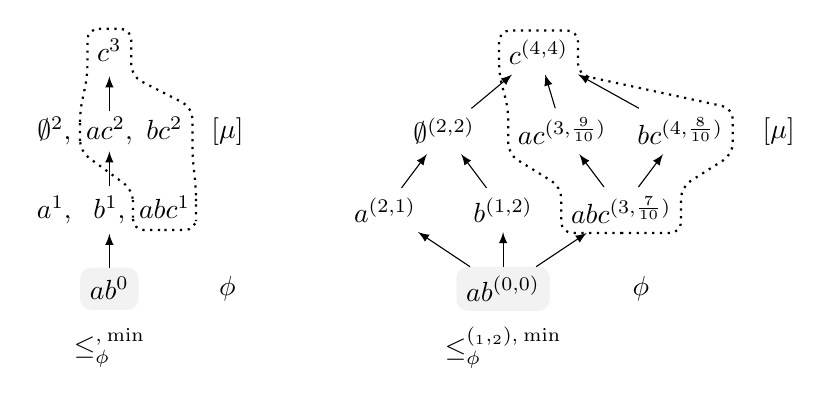
\begin{tikzpicture}
	%% total preorder
	\node at (0,-0.75){$\le^{\hamming,\:\min}_\phi$};
	
	\node at (0,0)(ab){$ab^0$};

	\node at (-0.7,1)(a){$\vphantom{b,}a^1,$};	
	\node at (0,1)(b){$b^1,$};
	\node[inner sep=0.2em] at (0.7,1)(abc){$abc^1\vphantom{,}$};

	\node at (-0.7,2)(e){$\emptyset^2,$};
	\node[inner sep=0.2em] at (0,2)(ac){$\vphantom{\emptyset}ac^2,$};
	\node at (0.7,2)(bc){$bc^2\vphantom{\emptyset,}$};

	\node at (0,3)(c){$\vphantom{b,}c^3$};

	\node at (1.5,0){$\mods{\phi}$};
	\node at (1.5,2){$[\mu]$};

	\path[-latex] (ab)edge(b)(b)edge(ac)(ac)edge(c);
	
	\fill[opacity=0.05, rounded corners = 4]
		(ab.south)--
		(ab.south east)--
		(ab.east)--
		(ab.north east)--
		(ab.north)--
		(ab.north west)--
		(ab.west)--
		(ab.south west)--
		(ab.south);

	\draw[thick, dotted, rounded corners=4]
		(abc.south)--
		(abc.south east)--
		(abc.east)--
		(abc.north east)--
		(bc.south east)--
		(bc.east)--
		(bc.north east)--
		(c.south east)--
		(c.east)--
		(c.north east)--
		(c.north)--
		(c.north west)--
		(c.west)--
		(c.south west)--
		(ac.north west)--
		(ac.west)--
		(ac.south west)--
		(abc.north west)--
		(abc.west)--
		(abc.south west)--
		(abc.south);

	%% partial preorder
	\node at (5,-0.75){$\le^{(\dd_{1},\dd_{2}),\:\min}_\phi$};

	\node at (5,0)(ab){$ab^{(0,0)}$};

	\node at (3.5,1)(a){$a^{(2,1)}$};	
	\node at (5,1)(b){$b^{(1,2)}$};
	\node at (6.5,1)(abc){$abc^{(3,\frac{7}{10})}$};

	\node at (4.25,2)(e){$\emptyset^{(2,2)}$};
	\node at (5.75,2)(ac){$ac^{(3,\frac{9}{10})}$};
	\node at (7.25,2)(bc){$bc^{(4,\frac{8}{10})}$};

	\node at (5.45,3)(c){$c^{(4,4)}$};

	\node at (6.75,0){$\mods{\phi}$};
	\node at (8.5,2){$[\mu]$};
	\path[-latex] 
		(ab)edge(a)(ab)edge(b)(ab)edge(abc)(a)edge(e)
		(b)edge(e)(abc)edge(ac)(abc)edge(bc)(e)edge(c)
		(ac)edge(c)(bc)edge(c);
	
	\fill[opacity=0.05, rounded corners = 4]
		(ab.south)--
		(ab.south east)--
		(ab.east)--
		(ab.north east)--
		(ab.north)--
		(ab.north west)--
		(ab.west)--
		(ab.south west)--
		(ab.south);

	\draw[thick, dotted, rounded corners=4]
		(abc.south)--
		(abc.south east)--
		(abc.east)--
		(abc.north east)--
		(bc.south east)--
		(bc.east)--
		(bc.north east)--
		(c.south east)--
		(c.east)--
		(c.north east)--
		(c.north)--
		(c.north west)--
		(c.west)--
		(c.south west)--
		(ac.north west)--
		(ac.west)--
		(ac.south west)--
		(abc.north west)--
		(abc.west)--
		(abc.south west)--
		(abc.south);
	\end{tikzpicture}
	\caption{
		A total preorder $\le^{\hamming,\:\min}_\phi$ 
		and a partial preorder $\le^{(\dd_{1},\dd_{2}),\:\min}_\phi$. 
		The distances from $\phi$ to each interpretation are written as superscripts next to each interpretation.
		Models of $\phi$ are shaded in gray, models of $\mu$ are in the region bounded by the dotted border. 
	}
	\label{fig:3-revision-dalal-partial}
\end{figure}

\begin{xmpl}{A monopoly on tool use no more}{3-revision-dmin}
	For the last time in this chapter, we look at the revision scenario from 
	Example \ref{ex:3-revision-basic-setup},
	for which $[\phi]=\{ab\}$ and $[\mu]=\{c,ac,bc,abc\}$.
	The preorder $\le_\phi^{\hamming,\:\min}$ generated 
	using Hamming distance and 
	the $\min$ aggregation function is depicted 
	on the left in Figure \ref{fig:3-revision-dalal-partial}.
	According to it we obtain that $[\phi\re^{\hamming,\:\min}\mu]=\min_{\le^{\hamming,\:\min}_\phi}[\mu]=\{abc\}$.
	Consider also 
	two quasi-distances $\dd_{1}$ and $\dd_{2}$ between interpretations that generate
	the partial preorder $\le_\phi^{(\dd_{1},\dd_{2}),\:\min}$ depicted on the right 
	in Figure \ref{fig:3-revision-dalal-partial}. 
	According to it we obtain 
	$[\phi\re^{(\dd_{1},\dd_{2}),\:\min}\mu]=\min_{\le^{(\dd_{1},\dd_{2}),\:\min}_\phi}[\mu]=\{abc\}$,
	which is the same result as for $\re^{\hamming,\:\min}$.

	In both cases, the revision operators arrive at the same conclusion
	that has ultimately prevailed in the primatology community: 
	the minimally disruptive response to Jane Goodall's findings is to 
	hold on to the beliefs that humans use tools and that chimpanzees are a different
	species from humans,
	but to accept that chimpanzees can use tools.
\end{xmpl}

We end this section by returning to a point that was made at its beginning.
The point is that, at least insofar as postulates $\ppr{1-8}$ are concerned,
the type of entity represented by $\phi$ and $\mu$
should be conceived as fluid, hovering somewhere in 
the space of cognitive attitudes an agent can have towards a generic set of issues,
but exclusive to neither of them in particular.
This is seen more clearly through the choice lens, 
embodied by Theorems \ref{thm:3-revision-repr-km-total} and \ref{thm:3-revision-repr-km-partial}):
postulates $\ppr{1-8}$ axiomatize preference maximizing behavior,
i.e., an operation that selects the best alternatives out of a 
set menu, biasing the judgment of what is best on the prior information available; 
this is behavior that is no more exclusive to beliefs than it is to actions
or bundles of goods, and it can be expected to be part of a rational agent's arsenal
in all of these cases.
The general appeal of framing rational behavior in this way
was understood early on in economics 
\cite{Nash1950,Arrow51,Chernoff54,RadnerM54,LuceR57,Hansson68,Sen69,Sen70,Herzberger73},
and is what lies, for Hans Rott, at the root of both theoretical and practical reason:

\begin{quote}
	The constraints [for rational or coherent choice]
	are shown to give rise to corresponding lists of  
	conditions for [\dots] revision and inference operations. 
	I take this to be strong evidence for the unity of 
	theoretical and practical reason, with the principles for 
	the former being special cases of principles for the latter. 
	\cite[p.~214]{Rott92}
\end{quote}

As mentioned before, the moral we want to draw from here 
is not that postulates $\ppr{1-8}$ are the last word in 
what constitutes rational behavior, but that they 
are parts of a larger framework that is worth exploring further.































\section{Update}\label{sec:3-update}
Revision, as we have seen in Section \ref{sec:3-revision},
works by choosing the best outcomes from the ones consistent 
with the new information,
or, in what is the same thing,
by discarding any outcomes from the new information
that are not optimal.
While this selection process makes sense in certain scenarios,
there are cases in which it ends up being too aggressive.

\begin{xmpl}{Keeping up with the humans, as an update task}{3-update-basic-setup}
	Consider the scenario in Example \ref{ex:1-update-motivation}.
	The variables that my automatic assistant keeps track of are 
	whether the temperature is above $15\si{\degree}$ C ($a$),
	whether the Wi-Fi is on after $21{:}00$ ($b$),
	and whether my friend is online after $21{:}00$ ($c$).
	The instructions my assistant is programmed to implement 
	are $\phi=a\land \lnot b$,
	whereas my observed pattern of behavior is represented by the formula 
	$\mu=(b\leftrightarrow c)$.
	The assistant would like to
	modify its list of instructions to accommodate my behavior,
	i.e., to change $\phi$ in accordance with $\mu$.
	In this case, it seems like the sensible answer is 
	to move from $\phi$ to $\phi' = a\land (b \leftrightarrow c)$,
	i.e., maintain temperature above $15\si{\degree}$ C and 
	leave the Wi-Fi on after $21{:}00$
	at exactly those times when my friend is online.
	Note that revision is not the appropriate operation here:
	since $\phi$ and $\mu$ are consistent, a typical revision operator would 
	return $\phi\land\mu\equiv a\land\lnot b\land \lnot c$:
	according to the logic of revision
	my smarthome would infer that, 
	since it is after $21{:}00$ and the	Wi-Fi is turned off, 
	then my friend must be offline.
\end{xmpl}

Example \ref{ex:3-update-basic-setup} illustrates the need for a belief change operator
that retains more information from the new information $\mu$
than a revision operator would normally do,
while still being biased by $\phi$.
The bias towards $\phi$, therefore,
should not be so strong as to render all but the 
absolute closest outcomes as unfeasible.
Update operators were introduced to do justice to 
this intuition \cite{KatsunoM91},
and we will see that they do so by modifying
the way in which models of $\mu$ are chosen 
for the final result.
In the rest of this section we will focus on the mechanics
of update, using the same methodology as the one used for
revision: postulates, preferences over outcomes, 
representation theorems and distances between interpretations.

% Update was originally introduced to model changes 
% in an agent's epistemic state when the state of the world changes,
% rather than when the agent receives new information 
% about a presumably static world \cite{KatsunoM91}.
% The remaining part of this section will employ the same methodology
% methodology to formalize the mechanism involved here.

\subsubsection{Postulates}
Like revision, update is a single-agent belief change operator.
Formally, an \emph{$\L$-update operator $\up$} 
is a function $\up\colon\L\times\L\rightarrow\L$,
taking as input 
two propositional formulas, 
denoted here by $\phi$ and $\mu$,
and standing in for the agent's prior information and the newly acquired 
information, respectively,
and returning a propositional formula,
denoted here by $\phi\up\mu$,
and standing for the agent's posterior information.
As with revision, $\phi$ and $\mu$ are nominally intended to be beliefs,
but in practice can be any of a number of cognitive attitudes an agent
can have toward a set of items.

Recall that a complete formula $\dot{\phi}$ is complete 
if $\dot{\phi}$ has exactly one model.
If $\up$ is an $\L$-update operator, 
the postulates $\up$ is expected to satisfy are, 
for any propositional formulas $\phi$, $\phi_{1}$, $\phi_{2}$,
complete formulas $\dot{\phi}$,
$\mu$, $\mu_{1}$ and $\mu_{2}$,
as follows:

\begin{description}
	\item[($\ppu{1}$)] $\phi\up\mu\models\mu$.
	
	\item[($\ppu{2}$)] If $\phi\models\mu$, then $\phi\up\mu\equiv\phi$.
	
	\item[($\ppu{3}$)] If $\phi$ and $\mu$ are satisfiable, then $\phi\up\mu$ is satisfiable.
	
	\item[($\ppu{4}$)] If $\phi_1\equiv\phi_2$ and $\mu_1\equiv\mu_2$, 
		then $\phi_1\up\mu_1\equiv\phi_2\up\mu_2$.
	
	\item[($\ppu{5}$)] $(\phi\up\mu_1)\land\mu_2\models\phi\up(\mu_1\land\mu_2)$.
	
	\item[($\ppu{6}$)] If $(\dot{\phi}\up\mu_1)\land\mu_2$ is consistent, 
		then $\dot{\phi}\up(\mu_1\land\mu_2)\models(\dot{\phi}\up\mu_1)\land\mu_2$.

	\item[($\ppu{7}$)] If $\phi\up\mu_1\models\mu_2$ and $\phi\up\mu_2\models\mu_1$, 
		then $\phi\up\mu_1\equiv\phi\up\mu_2$.
	
	\item[($\ppu{8}$)] If $\mu\equiv \mu_{1}\lor\mu_{2}$.
		then $(\dot{\phi}\up\mu_1)\land(\dot{\phi}\up\mu_2)\models\dot{\phi}\up\mu$.
	
	\item[($\ppu{9}$)] $(\phi_{1}\lor\phi_{2})\up\mu\equiv(\phi_1\up\mu)\lor(\phi_2\up\mu)$.
\end{description}

As for revision, postulate $\ppu{6}$ implies postulates $\ppu{7}$ and $\ppu{8}$,
and the plan with respect to their use is the same:
postulates $\ppu{7-8}$ are meant to be alternatives to $\ppu{6}$.
An update operator $\up$ is \emph{exhaustive} if it satisfies postulates $\ppu{1-6}$ and $\ppu{9}$,
and \emph{exclusive} if it satisfies postulates $\ppu{1-5}$ and $\ppu{7-9}$.

The numbering of the postulates is slightly different from the usual ordering 
\cite{KatsunoM91}, but the re-numbering is meant to highlight the close connection
to revision.
Indeed, note that postulates $\ppu{1}$ and $\ppu{3-8}$ are
esentially similar to the revision postulates $\ppr{1}$ and $\ppr{3-8}$
(see Section \ref{sec:3-revision}), with the only point of departure 
being that postulates $\ppu{6}$ and $\ppu{8}$ are meant to apply only 
to complete formulas $\dot{\phi}$.
What is more, if $\phi$ is a complete formula,
then postulates $\ppu{1-8}$ are entirely 
equivalent to revision postulates
$\ppr{1-8}$: this is true even for postulate $\ppu{2}$,
since if $\phi$ is complete then 
$\phi\land\mu$ and $\phi$ become equivalent
and the statement that $\phi\models\mu$
is equivalent to the statement that $\phi\land\mu$ is consistent.
This is an observation that has been made before \cite{PeppasNPFKP96}
but is worth stressing, since it provides 
insight into the working of an update operator:
on complete propositional formulas,
update according to postulates $\ppu{1-8}$
is just revision according to postulates $\ppr{1-8}$.

If $\phi$ is not complete, 
then postulates $\ppu{2}$ and $\ppu{9}$
kick in, and can be seen as new additions
to the toolbox of familiar postulates.
In this case postulate $\ppu{2}$ is a weaker version of the revision postulate
$\ppr{2}$, and regulates the way in which the prior information $\phi$
biases the update result.
Postulate $\ppu{9}$ specifies the way in which the update result
can be decomposed in results for more specific parts of the prior information $\phi$,
i.e., formulas $\phi_{1}$ and $\phi_{2}$
such that $\phi_{1}\lor \phi_{2}\equiv \phi$.
Ultimately, repeated application of postulate $\ppu{9}$ makes the result
for $\phi\up\mu$
entirely dependent on the update result for the complete formulas
that imply $\phi$.
More precisely, if $\px_v$ is an $\L$-proxy for the interpretation $v$,
i.e., a propositional formula such that $[\px_v]=\{v\}$,
then postulate $\ppu{9}$ is equivalent to the following postulate, 
applying for any propositional formulas $\phi$ and $\mu$:

\begin{description}
	\item[($\ppu{10}$)] $\phi\up\mu\equiv \bigvee_{v\in[\phi]}(\px_{v}\up\mu)$.
\end{description}

Postulate $\ppu{10}$ shows that $\phi\up\mu$ can be decomposed
in the results for $\px_{v}\up\mu$, for every $v\in[\phi]$. 
We will make extensive use of postulate $\ppu{9}$ and, even more so, 
of its equivalent reformulation $\ppu{10}$, 
in what is to follow.

\begin{xmpl}{Update is not revision}{3-update-postulates}
	For the setting in Example \ref{ex:3-update-basic-setup},
	where $\phi = a\land\lnot b$
	and $\mu=b\leftrightarrow c$,
	we have that $\phi\land\mu$ is consistent,
	but $\phi\not\models\mu$.
	Thus, whereas a revision operator satisfying postulate $\ppr{2}$ 
	would require the result to be $\phi\land\mu$,
	the update postulate $\ppu{2}$ places no constraints in this case.

	Since $[\phi]=\{a,ac\}$, 
	postulate $\ppu{9}$ (or $\ppu{10}$) requires that 
	$\phi\up\mu\equiv(\px_{a}\up\mu)\lor(\px_{ac}\up\mu)$.
\end{xmpl}

As with the revision postulate $\ppr{8}$ in Section \ref{sec:3-revision},
postulate $\ppu{8}$ has also been slightly re-phrased:
normally there would be no reference to $\mu$, 
with $\mu_{1}\lor\mu_{2}$ written instead.
But here, as well, the difference from the usual statement 
is merely stylistic. 
The role of this re-phrasing is only to make life easier
in Chapter \ref{ch:6}.

\subsubsection{Preferences over outcomes}
Postulate $\ppu{9}$, and even more so postulate $\ppu{10}$,
show that what gets chosen in $\phi\up\mu$ is determined 
by what gets chosen in $\px_{v}\up\mu$,
for every $v\in[\mu]$.
Furthermore, update for complete formulas is just revision.
This provides a useful hint for how to model update as a choice
procedure:
we will use an
\emph{$\L_{\comp}$-assignment $\as$ on interpretations}, 
which is a function $\as\colon\L_{\comp}\rightarrow 2^{\U\times\U}$,
taking as input a complete formula $\dot{\phi}$ and returning
a binary relation on interpretations, 
interpreted, as for revision, as a plausibility ranking.
An $\L_{\comp}$ assignment corresponds to 
what has been called in the literature as a \emph{pointwise assignment}
\cite{KatsunoM91}.

As expected, we are keen on $\as$ satisfying some desirable properties,
and the properties we are interested in are as follows, 
for any complete propositional formulas $\dot{\phi}$, $\dot{\phi_{1}}$, $\dot{\phi_{2}}$
and interpretations $w$, $v$, $w_1$ and $w_2$:

\begin{description}
	\item[($\oou{1}$)] $w\le_{\dot{\phi}} w$.
	\item[($\oou{2}$)] If $w_1\le_{\dot{\phi}} w_2$ and $w_2\le_{\dot{\phi}} w_3$, 
		then $w_1\le_{\dot{\phi}} w_3$.
	\item[($\oou{3}$)] $w_1\le_{\dot{\phi}} w_2$ or $w_2\le_{\dot{\phi}} w_1$.
	\item[($\oou{4}$)] If $\dot{\phi_1}\equiv \dot{\phi_2}$, then it holds that if  $w_1\le_{\dot{\phi_1}}w_2$, then $w_1\le_{\dot{\phi_2}}w_2$. 
	\item[($\oou{5}$)] If $[\dot{\phi}]=\{v\}$ and $w\neq v$, then $v<_{\dot{\phi}} w$.
\end{description}

Properties $\oou{1-4}$ are the same as properties $\oor{1-4}$,
except that they are particularized to complete formulas. 
They say, in effect, that $\le_{\dot{\phi}}$ is a preorder (properties $\oou{1-2}$),
additionally total (property $\oou{3}$)
and syntax insensitive (property $\oou{4}$),
for any complete propositional formula $\dot{\phi}$.
Property $\oou{5}$ conveys the same message as properties $\oor{5-7}$:
models of $\dot{\phi}$ are the unique minimal elements in $\le_{\dot{\phi}}$,
but, as $\dot{\phi}$ has only one model,
the distinctions inherent in properties $\oor{5-7}$ are not needed.
We are left, in this case, with the simpler property $\oou{5}$.

\begin{figure}\centering
	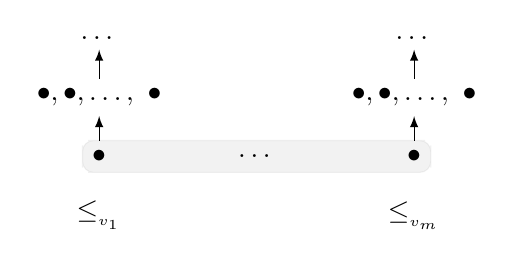
\begin{tikzpicture}
		\node at (0,-0.75){$\le_{\px_{v_{1}}}$};
		\node at (0,0)(01){$\bullet$};
		\node at (0,0.75)(1){$\bullet,\bullet,\dots,~\bullet$};
		\node at (0,1.5)(2){\dots};
		\path[-latex] (01) edge (1)(1) edge (2);
		
		\node at (2,0){\dots};

		\node at (4,-0.75){$\le_{\px_{v_{m}}}$};
		\node at (4,0)(0m){$\bullet$};
		\node at (4,0.75)(1){$\bullet,\bullet,\dots,~\bullet$};
		\node at (4,1.5)(2){\dots};
		\path[-latex] (0m) edge (1)(1) edge (2);

		\fill[draw, opacity=0.05, rounded corners=4]
			(0m.south)--
			(01.south)--
			(01.south west)--
			(01.west)--
			(01.north west)--
			(01.north)--
			(0m.north)--
			(0m.north east)--
			(0m.east)--
			(0m.south east)--
			(0m.south);	
	\end{tikzpicture}
	\caption{
		A schematic depiction of total preorders $\le_{\px_{v_i}}$,
		for $[\phi]=\{v_1,\dots,v_m\}$,
		in a total u-faithful assignment. 
		Bullets stand, as before, for interpretations.
		Each model of $\phi$ (placed in the shaded gray region) 
		generates its own total preorder on interpretations.
	}
	\label{fig:3-update-ufaithful-schematic}
\end{figure}

An $\L_{\comp}$-assignment $\as$ on interpretations is 
\emph{partial} if it satisfies properties $\oou{1-2}$,
\emph{total} if it satisfies properties $\oou{1-3}$,
syntax insensitive if it satisfies property $\oou{4}$
and \emph{u-faithful} if it satisfies property $\oou{5}$.
A schematic illustration of preorders in a total u-faithful
assignment is given in Figure \ref{fig:3-update-ufaithful-schematic}.

\subsubsection{Update as choice over outcomes}
Seeing update as a choice procedure over outcomes
involves putting together the two perspectives introduced
in the previous paragraphs: the logical postulates, on the
one side, and the plausibility rankings on interpretations, on the other.
As with revision, plausibility rankings can be used to guide update,
as well as be inferred from update behavior.

Thus, keeping in mind that
$\px_{v}$ is a propositional formula such that $[\px_{v}]=\{v\}$,
then, given an $\L_{\comp}$-assignment $\as$ on interpretations,
the \emph{$\as$-induced update operator $\up^{\as}$}
is defined, for any propositional formulas $\phi$ and $\mu$,
by taking:
$$
[\phi\up^{\as}\mu] \defeq \bigcup_{v\in[\phi]}\min_{\le_{\px_{v}}}[\mu].
$$
Conversely, given an $\L$-update operator $\up$,
and a complete propositional formula $\dot{\phi}$,
the \emph{exhaustive $\up$-revealed plausibility relation $\le^\exh_{\dot{\phi}}$} 
and the \emph{exclusive $\up$-revealed plausibility relation $\le^\exc_{\dot{\phi}}$} 
are defined, for any interpretations $w_1$ and $w_2$, respectively, as:
\begin{align*}
	w_1\le^\exh_{\dot{\phi}} w_2 &~\text{if}~w_1\in[\dot{\phi}\re\px_{1,2}],\\
	w_1\le^\exc_{\dot{\phi}} w_2 &~\text{if}~w_1\in[\dot{\phi}\re\px_{1,2}]~\text{and}~w_2\notin[\dot{\phi}\re\px_{1,2}].
\end{align*}
The \emph{exhaustive revealed $\L_{\comp}$-assignment $\as^\exh$} 
and \emph{exclusive revealed $\L_{\comp}$-assignment $\as^\exc$} are obtained
by taking $\as^\exh\!\!(\dot{\phi})=\le^\exh_{\dot{\phi}}$ and $\as^\exc\!\!(\dot{\phi})=\le^\exc_{\dot{\phi}}$, 
for any complete propositional formula $\dot{\phi}$.
The guiding intuition here is the same as for the exhaustive and exclusive revealed
assignments in revision.

\begin{figure}\centering
	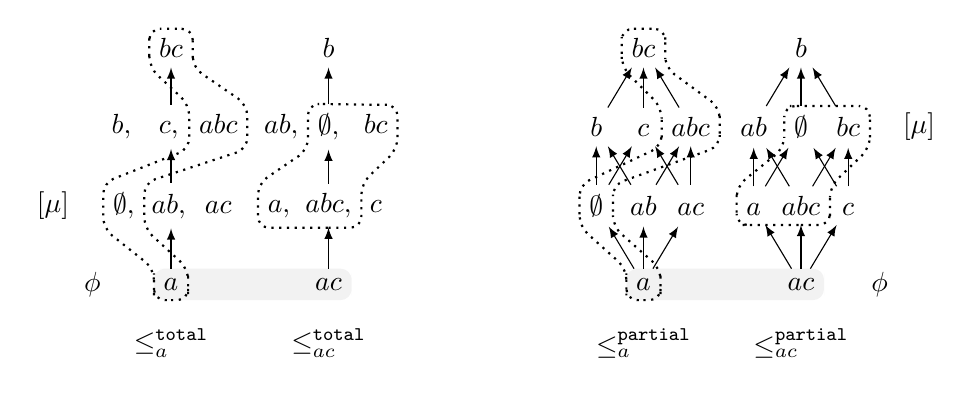
\begin{tikzpicture}
		%% Total preorders
		%% first preorders
		\node at (0,-0.75){$\le^{\mathtt{total}}_{a}$};

		\node at (0,0)(a1){$a$};

		\node at (-0.6,1)(e){$\emptyset,$};
		\node at (0,1)(ab){$ab,\vphantom{\emptyset}$};
		\node at (0.6,1)(ac){$ac\vphantom{\emptyset,}$};
	
		\node at (-0.6,2)(b){$b,\vphantom{b}$};	
		\node at (0,2)(c){$c,\vphantom{b}$};
		\node at (0.6,2)(abc){$abc\vphantom{,}$};		

		\node at (0,3)(bc){$bc$};

		% \node at (1.5,0){$\mods{\phi}$};
		% \node at (1.5,2){$[\mu]$};
	
		\path[-latex] (a1) edge (ab)(ab)edge(c)(c)edge(bc);
		
		\draw[thick, dotted, rounded corners=4]
			(a1.south)--
			(a1.south east)--
			(a1.east)--
			(a1.north east)--
			(e.south east)--
			(e.east)--
			(e.north east)--
			(abc.south east)--
			(abc.east)--
			(abc.north east)--
			(bc.south east)--
			(bc.east)--
			(bc.north east)--
			(bc.north)--
			(bc.north west)--
			(bc.west)--
			(bc.south west)--
			(abc.north west)--
			(abc.west)--
			(abc.south west)--
			(e.north west)--
			(e.west)--
			(e.south west)--
			(a1.north west)--
			(a1.west)--
			(a1.south west)--
			(a1.south);

		%% Second preorder
		\node at (2,-0.75){$\le^{\mathtt{total}}_{ac}$};

		\node at (2,0)(ac1){$ac$};

		\node at (1.4,1)(a){$a,\vphantom{b,}$};
		\node at (2,1)(abc){$abc,$};
		\node at (2.6,1)(c){$c\vphantom{b,}$};
	
		\node at (1.4,2)(ab){$ab,$};
		\node at (2,2)(e){$\emptyset,$};	
		\node at (2.6,2)(bc){$bc\vphantom{,}$};		

		\node at (2,3)(b){$b$};

		\node at (-1,0){$\mods{\phi}$};
		\node at (-1.5,1){$[\mu]$};
	
		\path[-latex] (ac1) edge (abc)(abc)edge(e)(e)edge(b);
		
		\draw[thick, dotted, rounded corners=4]
			(abc.south)--
			(abc.south east)--
			(abc.east)--
			(abc.north east)--
			(bc.south east)--
			(bc.east)--
			(bc.north east)--
			(bc.north)--
			(e.north)--
			(e.north west)--
			(e.west)--
			(e.south west)--
			(a.north west)--
			(a.west)--
			(a.south west)--
			(a.south)--
			(abc.south);
		\fill[opacity=0.05, rounded corners=4]
			(a1.south)--
			(ac1.south)--
			(ac1.south east)--
			(ac1.east)--
			(ac1.north east)--
			(ac1.north)--
			(a1.north)--
			(a1.north west)--
			(a1.west)--
			(a1.south west)--
			(a1.south);


		%%%%%%%%%%%%%%%%%%%%%
		%% Partial preorders
		%% first preorder

		\node at (6,-0.75){$\le^{\mathtt{partial}}_{a}$};

		\node at (6,0)(a1){$a$};

		\node at (5.4,1)(e){$\emptyset$};
		\node at (6,1)(ab){$ab\vphantom{\emptyset}$};
		\node at (6.6,1)(ac){$ac\vphantom{\emptyset}$};
	
		\node at (5.4,2)(b){$b\vphantom{b}$};	
		\node at (6,2)(c){$c\vphantom{b}$};
		\node at (6.6,2)(abc){$abc$};		

		\node at (6,3)(bc){$bc$};

		% \node at (1.5,0){$\mods{\phi}$};
		% \node at (1.5,2){$[\mu]$};
	
		\path[-latex] 
			(a1)edge(e)(a1)edge(ab)(a1)edge(ac) 
			(e)edge(b)(e)edge(c)
			(ab)edge(b)(ab)edge(abc)
			(ac)edge(c)(ac)edge(abc)
			(b)edge(bc)(abc)edge(bc)(c)edge(bc);
		
		\draw[thick, dotted, rounded corners=4]
			(a1.south)--
			(a1.south east)--
			(a1.east)--
			(a1.north east)--
			(e.south east)--
			(e.east)--
			(e.north east)--
			(abc.south east)--
			(abc.east)--
			(abc.north east)--
			(bc.south east)--
			(bc.east)--
			(bc.north east)--
			(bc.north)--
			(bc.north west)--
			(bc.west)--
			(bc.south west)--
			(abc.north west)--
			(abc.west)--
			(abc.south west)--
			(e.north west)--
			(e.west)--
			(e.south west)--
			(a1.north west)--
			(a1.west)--
			(a1.south west)--
			(a1.south);

		%% Second preorder
		\node at (8,-0.75){$\le^{\mathtt{partial}}_{ac}$};

		\node at (8,0)(ac1){$ac$};

		\node at (7.4,1)(a){$a\vphantom{b}$};
		\node at (8,1)(abc){$abc$};
		\node at (8.6,1)(c){$c\vphantom{b}$};

		\node at (7.4,2)(ab){$ab\vphantom{\emptyset}$};
		\node at (8,2)(e){$\emptyset$};	
		\node at (8.6,2)(bc){$bc\vphantom{\emptyset}$};		

		\node at (8,3)(b){$b$};

		\node at (9,0){$\mods{\phi}$};
		\node at (9.5,2){$[\mu]$};
	
		\path[-latex] 
			(ac1)edge(a)(ac1) edge (abc)(ac1)edge(c)
			(a)edge(ab)(a)edge(e)
			(abc)edge(ab)(abc)edge(bc)
			(c)edge(e)(c)edge(bc)
			(ab)edge(b)(e)edge(b)(bc)edge(b);
		
		\draw[thick, dotted, rounded corners=4]
			(abc.south)--
			(abc.south east)--
			(abc.east)--
			(abc.north east)--
			(bc.south east)--
			(bc.east)--
			(bc.north east)--
			(bc.north)--
			(e.north)--
			(e.north west)--
			(e.west)--
			(e.south west)--
			(a.north west)--
			(a.west)--
			(a.south west)--
			(a.south)--
			(abc.south);
		\fill[opacity=0.05, rounded corners=4]
			(a1.south)--
			(ac1.south)--
			(ac1.south east)--
			(ac1.east)--
			(ac1.north east)--
			(ac1.north)--
			(a1.north)--
			(a1.north west)--
			(a1.west)--
			(a1.south west)--
			(a1.south);
		\end{tikzpicture}
	\caption{
		Total and partial preorders 
		$\le^{\mathtt{total}}_{\px_{v}}$ 
		and
		$\le^{\mathtt{partial}}_{\px_{v}}$,
		for $[\phi]=\{a,ac\}$
		and $v\in[\phi]$,
		assigned by a total u-faithful assignment $\as^{\mathtt{total}}$
		and a partial u-faithful assignment $\as^{\mathtt{partial}}$,
		respectively.
		Models of $\phi$ are in the shaded gray regions.
		The new information is $\mu$,
		with $[\mu]=\{\emptyset,a,bc,abc\}$.
		The result of updating $\phi$ by $\mu$
		using the assignment $\as^{\mathtt{total}}$ amounts to taking
		the best models of $\mu$ from the preorders associated to 
		each model of $\phi$,
		i.e., from $\le^{\mathtt{total}}_{a}$ and from 
		$\le^{\mathtt{total}}_{ac}$.
		The same strategy applies to $\as^{\mathtt{partial}}$.
	}
	\label{fig:3-update-preorder-operator-interplay}
\end{figure}	

\begin{xmpl}{Keeping up with the humans, using assignments}{3-update-preorder-operator-interplay}
	For the setting in Example \ref{ex:3-update-basic-setup},
	with 
	$[\phi]=\{a,ac\}$ and $[\mu]=\{\emptyset,a,bc,abc\}$,
	consider two assignments:
	a total r-faithful assignment $\as^{\mathtt{total}}$
	and a partial r-faithful assignment $\as^{\mathtt{partial}}$,
	generating the preorders
	$\le^{\mathtt{total}}_{\px_{v}}$ 
	and
	$\le^{\mathtt{partial}}_{\px_{v}}$
	in Figure \ref{fig:3-update-preorder-operator-interplay},
	for $v\in[\phi]$.
	These assignments generate the update operators
	$\up^{\mathtt{total}}$ and $\up^{\mathtt{partial}}$,
	respectively,
	according to which:
	\begin{align*}
		[\phi\up^{\mathtt{total}}\mu] 												   	&
		=\min_{\le^{\mathtt{total}}_{a}}[\mu]\cup\min_{\le^{\mathtt{total}}_{ac}}[\mu] 	\\
																						   &
		= \{a,abc\}\\
		&= \min_{\le^{\mathtt{partial}}_{a}}[\mu]\cup\min_{\le^{\mathtt{partial}}_{ac}}[\mu]\\
		&=[\phi\up^{\mathtt{partial}}\mu].
	\end{align*}

	Conversely, to find out the agent's ranking of, say, outcomes $b$ and $c$,
	if its initial belief were the complete formula $\px_{a}$,
	with $[\px_{a}]=\{a\}$,
	we would look at the result of $\px_{a}\up\px_{b,c}$.
	Supposing that the result is 
	$[\px_{a}\up\px_{b,c}]=\{b,c\}$,
	then according to the exhaustive $\up$-revealed $\L_{\comp}$-assignment,
	we would conclude that $b\approx^{\exh}_{\px_{a}} c$,
	whereas according to the exclusive $\up$-revealed $\L_{\comp}$-assignment
	we would conclude that neither $b\le^{\exc}_{\px_{a}} c$ nor
	$c\le^{\exc}_{\px_{a}} b$.
	These results are in accordance with
	$\le^{\mathtt{total}}_{\px_{a}}$ 
	and
	$\le^{\mathtt{partial}}_{\px_{a}}$
	as in Figure \ref{fig:3-update-preorder-operator-interplay}.
\end{xmpl}

If $\up$ is an $\L$-update operator
and $\as$ is an $\L_{\comp}$-assignment on interpretations,
then \emph{$\as$ represents $\up$}
(and \emph{$\up$ is represented by $\as$})
if, for any propositional formulas $\phi$ and $\mu$, it holds that 
$[\phi\up\mu]=\bigcup_{v\in[\phi]}\min_{\le_{\px_{v}}}[\mu]$.

As with revision, we obtain two representation results 
for update operators satisfying either postulates $\ppu{1-6}$ and $\ppu{9}$,
or postulates $\ppu{1-5}$, $\ppu{7-9}$,
one for total preorders and one for partial preorders.
The first result is in terms of total preorders

\begin{thm}{\cite{KatsunoM91}}{3-update-repr-km-total}
	An update operator $\up$ satisfies postulates $\ppu{1-6}$ and $\ppu{9}$ 
	(i.e., is exhaustive)
	if and only if
	there exists an 
	$\L_{\comp}$-assignment $\as$ on interpretations
	that satisfies properties $\oou{1-5}$
	(i.e., is total, syntax insensitive and u-faithful)
	and that represents the operator $\up$.
\end{thm}
\begin{prf*}{}{}%
	The $\L_{\comp}$-assignment representing $\up$ is exactly 
	the $\up$-revealed exhaustive assignment $\as^{\exh}$, 
	and the proof that it satisfies properties $\oou{1-5}$
	and that $[\dot{\phi}\up\mu] = \min_{\le^{\exh}_{\dot{\phi}}}[\mu]$,
	for any formula $\mu$ and complete formula $\dot{\phi}$,
	is essentially similar to the proof for the exhaustive
	revealed assignment of a revision operator 
	(see Theorems \ref{thm:3-revision-repr-total} and \ref{thm:3-revision-repr-R2-total}).
	For the last step, i.e., showing that 	
	$[\phi\up\mu]=\bigcup_{v\in[\phi]}\min_{\le^{\exh}_{\px_{v}}}[\mu]$,
	postulate $\ppu{9}$ (or, more precisely, postulate $\ppu{10}$) is used.
\end{prf*}

The accompanying result trades postulate $\ppu{6}$ for $\ppu{7-8}$
to obtain partial preorders instead of total preorders.

\begin{thm}{\cite{KatsunoM91}}{3-update-repr-km-partial}
	An update operator $\up$ satisfies postulates $\ppu{1-5}$, $\ppu{7-8}$ and $\ppu{9}$ 
	(i.e., is exclusive)
	if and only if
	there exists an 
	$\L_{\comp}$-assignment $\as$ on interpretations
	that satisfies properties $\oou{1-2}$ and $\oou{4-5}$
	(i.e., is partial, syntax insensitive and u-faithful)
	and that represents the operator $\up$.
\end{thm}
\begin{prf*}{}{}%
	The $\L_{\comp}$-assignment representing $\up$ is exactly 
	the $\up$-revealed exclusive assignment $\as^{\exc}$, 
	and the proof that it satisfies properties $\oou{1-2}$ and $\oou{4-5}$
	and that $[\dot{\phi}\up\mu] = \min_{\le^{\exc}_{\dot{\phi}}}[\mu]$,
	for any formula $\mu$ and complete formula $\dot{\phi}$,
	is essentially similar to the proof for the exclusive
	revealed assignment of a revision operator 
	(see Theorems \ref{thm:3-revision-repr-partial} and \ref{thm:3-revision-repr-R2-partial}).
	For the last step, i.e., showing that 	
	$[\phi\up\mu]=\bigcup_{v\in[\phi]}\min_{\le^{\exc}_{\px_{v}}}[\mu]$,
	postulate $\ppu{9}$ (or, more precisely, postulate $\ppu{10}$) is used.
\end{prf*}

As with revision, we can refine the analysis 
by separating postulate $\ppu{2}$ from the rest of the postulates:
what we obtain, then, are update operators represented
by either total or partial $\L_{\comp}$-assignments that are syntax insensitive
but do not, however, satisfy property $\oou{5}$ (i.e., are not u-faithful).
In other words, postulate $\ppu{2}$ regulates, as for revision,
the position of the model of a complete formula $\dot{\phi}$
in $\le_{\dot{\phi}}$ and its absence means that this model can
be placed anywhere in $\le_{\dot{\phi}}$.

\subsubsection{Total and partial preorders}
Theorems \ref{thm:3-update-repr-km-total} and \ref{thm:3-update-repr-km-partial}
tell us that to obtain update operators that satisfy postulates $\ppu{1-9}$
we must look for ways of generating rankings on interpretations.
These rankings are supposed to depend on a single interpretation,
so the tried and tested method of using a quasi-distance $\dd$ 
together with an aggregation function $\agg$
works here smoothly (see Section \ref{sec:2-distances}). 
As for revision, we will take $\agg$ in this section 
to be the $\min$ aggregation function.
Thus, if $\dd$ is a quasi-distance between interpretations
and $v$, $w_1$ and $w_2$ are interpretations, the
$(\dd,\:\min)$-induced ranking $\le^{\dd,\:\min}_{\px_{v}}$
is obtained by taking:
$$
	w_1\le^{\dd,\:\min}_{\px_{v}} w_2~\text{if}~\dd(v,w_1)\le \dd(v,w_2).
$$
If $\dd$ is a quasi-distance,
the \emph{${(\dd,\:\min)}$-induced assignment $\as^{\dd,\:\min}$} is obtained,
similarly as for revision, by taking 
$\as^{\dd,\:\min}\!\!(\dot{\phi})=\le_{\dot{\phi}}^{\dd,\:\min}$,
for any complete propositional formula $\dot{\phi}$.
The \emph{${(\dd,\:\min)}$-induced $\L$-update operator $\up^{\dd,\:\min}$} 
is the operator induced by the $\L_{\comp}$-assignment $\as^{\dd,\:\min}$.
The assignments that are generated in this way turn out to be 
total, syntax insensitive and u-faithful.

\begin{prp}{}{3-update-d-induced-preorder}
	If $\dd$ is a quasi-distance between interpretations 
	and $\dot{\phi}$ is a complete propositional formula, 
	the ${(\dd,\:\min)}$-induced ranking $\le^{\dd,\:\min}_{\dot{\phi}}$ 
	satisfies properties $\oor{1-5}$, 
	i.e., $\le^{\dd,\:\min}_{\dot{\phi}}$ is total,
	syntax insensitive and u-faithful.
\end{prp}
\begin{prf*}{}{}%
	Entirely similar to the proof for Proposition \ref{prop:3-revision-d-induced-preorder}.
\end{prf*}

Proposition \ref{prop:3-update-d-induced-preorder} 
implies that the $({\dd,\:\min})$-induced assignment $\as^{\dd,\:\min}$ 
is total, u-faithful and syntax insensitive, 
which, by Theorem \ref{thm:3-update-repr-km-total}, 
implies that the $({\dd,\:\min})$-induced update operator 
$\up^{\dd,\:\min}$ satisfies postulates $\ppu{1-9}$.

\begin{crl}{}{3-update-d-induced-operator}
	If $\dd$ is a quasi-distance between interpretations, 
	the $(\dd,\:\min)$-induced update operator $\up^{\dd,\:\min}$ 
	satisfies postulates $\ppu{1-6}$ and $\ppu{9}$.
\end{crl}

The operators generated using Hamming distance $\dd_{\hamming}$
and drastic distance $\dd_{\drastic}$
are denoted $\up^{\hamming,\:\min}$ and $\up^{\drastic,\:\min}$,
respectively.
We will refer to $\up^{\hamming,\:\min}$ as \emph{Forbus's operator} \cite{Forbus89}, 
and to $\up^{\drastic,\:\min}$ as the \emph{drastic update operator}.

Since any update operator that satisfies postulates $\ppu{1-6}$
also satisfies postulates $\ppu{7-8}$, Forbus's operator and the drastic 
update operator work as examples for both exhaustive and exclusive operators.
To obtain purely exclusive operators we could use the same technique as in 
Section \ref{sec:3-revision}, i.e., employ two quasi-distances $\dd_1$ and $\dd_2$.
However, we will present a different type of operator here.
If $w_1$ and $w_2$ are two interpretations, 
the \emph{symmetric difference $w_1\triangle w_2$ between $w_1$ and $w_2$} is defined as:
$$
	w_1\triangle w_2 = (w_1\setminus w_2)\cup(w_2\setminus w_1).
$$
We have already used the cardinality of the symmetric difference between $w_1$ and $w_2$
to define the Hamming distance between $w_1$ and $w_2$,
but here we will focus on the actual contents of the symmetric difference.
Thus,
if $v$, $w_1$ and $w_2$ are interpretations, the
$\symdiff$-induced ranking $\le^{\symdiff}_{\px_{v}}$
is obtained by taking:
$$
	w_1\le^{\symdiff}_{\px_{v}} w_2~\text{if}~(v\triangle w_1) \subseteq (v\triangle w_2).
$$
If $\dd$ is a quasi-distance,
the \emph{$\symdiff$-induced $\L_{\comp}$-assignment $\as^{\symdiff}$} is obtained,
by taking 
$\as^{\symdiff}\!\!(\dot{\phi})=\le_{\dot{\phi}}^{\symdiff}$,
for any complete propositional formula $\dot{\phi}$.
The \emph{$\symdiff$-induced $\L$-update operator $\up^{\symdiff}$},
is the operator induced by the $\L_{\comp}$-assignment $\as^{\symdiff}$.
The $\symdiff$-induced $\L$-update operator $\up^{\symdiff}$
is also called Winslett's operator \cite{Winslett05}.

The $\L_{\comp}$-assignment $\as^{\symdiff}$
turns out to be 
partial, syntax insensitive and u-faithful.

\begin{prp}{}{3-update-symdiff-induced-preorder}
	If $\dot{\phi}$ is a complete propositional formula, 
	the $\symdiff$-induced ranking $\le^{\symdiff}_{\dot{\phi}}$ 
	satisfies properties $\oou{1-2}$ and $\oou{4-5}$, 
	i.e., $\le^{\symdiff}_{\dot{\phi}}$ is a partial preorder 
	on interpretations that
	is syntax insensitive and 
	makes the model of $\dot{\phi}$ 
	the $\le^{\symdiff}_{\dot{\phi}}$-minimal element.
\end{prp}
\begin{prf*}{}{}%
	It is straightforward to see that $\le_{\dot{\phi}}^{\symdiff}$ satisfies 
	properties $\oou{1-2}$ and $\oou{4}$. 
	Notice, now, that if $w$ is an interpretation such that $v\neq w$,
	then $v\triangle w\neq\emptyset$, whereas $v\triangle v = \emptyset$.
	Thus, for any $w\neq v$, it holds that 
	$v<^{\symdiff}_{\px_v}w$, which shows that $\le^{\symdiff}_{\px_v}$
	satisfies property $\oou{5}$.
\end{prf*}

Proposition \ref{prop:3-update-symdiff-induced-preorder} 
implies that the $\symdiff$-induced assignment $\as^{\symdiff}$ 
is partial, u-faithful and syntax insensitive, 
which, by Theorem \ref{thm:3-update-repr-km-partial}, 
implies that the $\symdiff$-induced update operator 
$\up^{\symdiff}$ satisfies postulates $\ppu{1-5}$ and $\ppu{7-9}$.

\begin{crl}{}{3-update-symdiff-induced-operator}
	The $\symdiff$-induced update operator $\up^{\symdiff}$ 
	satisfies postulates $\ppu{1-6}$ and $\ppu{9}$.
\end{crl}

\begin{figure}\centering
	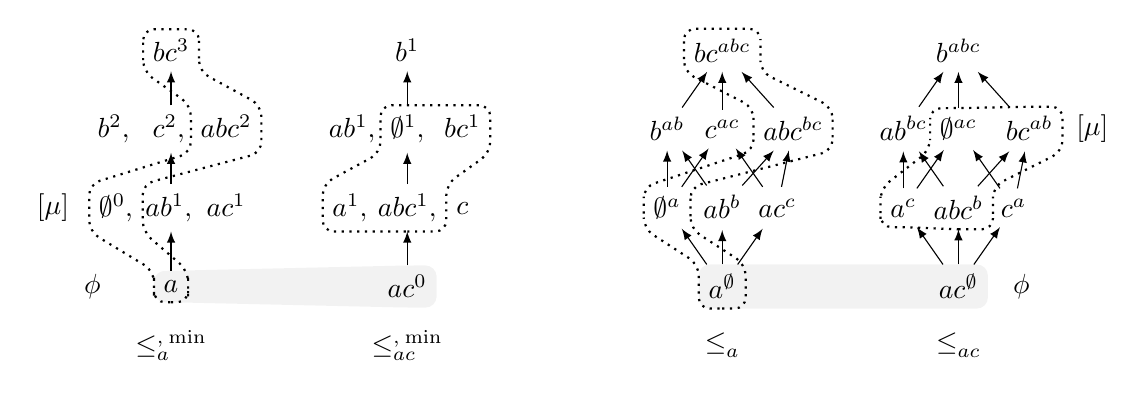
\begin{tikzpicture}
		%% Total preorders
		%% first preorders
		\node at (0,-0.75){$\le^{\hamming,\:\min}_{a}$};

		\node at (0,0)(a1){$a$};

		\node at (-0.7,1)(e){$\emptyset^0,$};
		\node at (0,1)(ab){$ab^1,\vphantom{\emptyset}$};
		\node at (0.7,1)(ac){$ac^1\vphantom{\emptyset,}$};
	
		\node at (-0.7,2)(b){$b^2,\vphantom{b}$};	
		\node at (0,2)(c){$c^2,\vphantom{b}$};
		\node at (0.7,2)(abc){$abc^2\vphantom{,}$};		

		\node at (0,3)(bc){$bc^3$};

		% \node at (1.5,0){$\mods{\phi}$};
		% \node at (1.5,2){$[\mu]$};
	
		\path[-latex] (a1) edge (ab)(ab)edge(c)(c)edge(bc);
		
		\draw[thick, dotted, rounded corners=4]
			(a1.south)--
			(a1.south east)--
			(a1.east)--
			(a1.north east)--
			(e.south east)--
			(e.east)--
			(e.north east)--
			(abc.south east)--
			(abc.east)--
			(abc.north east)--
			(bc.south east)--
			(bc.east)--
			(bc.north east)--
			(bc.north)--
			(bc.north west)--
			(bc.west)--
			(bc.south west)--
			(abc.north west)--
			(abc.west)--
			(abc.south west)--
			(e.north west)--
			(e.west)--
			(e.south west)--
			(a1.north west)--
			(a1.west)--
			(a1.south west)--
			(a1.south);

		%% Second preorder
		\node at (3,-0.75){$\le^{\hamming,\:\min}_{ac}$};

		\node at (3,0)(ac1){$ac^0$};

		\node at (2.3,1)(a){$a^1,\vphantom{b,}$};
		\node at (3,1)(abc){$abc^1,$};
		\node at (3.7,1)(c){$c\vphantom{b,}$};
	
		\node at (2.3,2)(ab){$ab^1,$};
		\node at (3,2)(e){$\emptyset^1,$};	
		\node at (3.7,2)(bc){$bc^1\vphantom{,}$};		

		\node at (3,3)(b){$b^1$};

		\node at (-1,0){$\mods{\phi}$};
		\node at (-1.5,1){$[\mu]$};
	
		\path[-latex] (ac1) edge (abc)(abc)edge(e)(e)edge(b);
		
		\draw[thick, dotted, rounded corners=4]
			(abc.south)--
			(abc.south east)--
			(abc.east)--
			(abc.north east)--
			(bc.south east)--
			(bc.east)--
			(bc.north east)--
			(bc.north)--
			(e.north)--
			(e.north west)--
			(e.west)--
			(e.south west)--
			(a.north west)--
			(a.west)--
			(a.south west)--
			(a.south)--
			(abc.south);
		\fill[opacity=0.05, rounded corners=4]
			(a1.south)--
			(ac1.south)--
			(ac1.south east)--
			(ac1.east)--
			(ac1.north east)--
			(ac1.north)--
			(a1.north)--
			(a1.north west)--
			(a1.west)--
			(a1.south west)--
			(a1.south);


		%%%%%%%%%%%%%%%%%%%%%
		%% Partial preorders
		%% first preorder

		\node at (7,-0.75){$\le^{\symdiff}_{a}$};

		\node at (7,0)(a1){$a^{\emptyset}$};

		\node at (6.3,1)(e){$\emptyset^{a}$};
		\node at (7,1)(ab){$ab^{b}\vphantom{\emptyset}$};
		\node at (7.7,1)(ac){$ac^{c}\vphantom{\emptyset}$};
	
		\node at (6.3,2)(b){$b^{ab}\vphantom{b}$};	
		\node at (7,2)(c){$c^{ac}\vphantom{b}$};
		\node at (7.9,2)(abc){$abc^{bc}$};		

		\node at (7,3)(bc){$bc^{abc}$};

		% \node at (1.5,0){$\mods{\phi}$};
		% \node at (1.5,2){$[\mu]$};
	
		\path[-latex] 
			(a1)edge(e)(a1)edge(ab)(a1)edge(ac) 
			(e)edge(b)(e)edge(c)
			(ab)edge(b)(ab)edge(abc)
			(ac)edge(c)(ac)edge(abc)
			(b)edge(bc)(abc)edge(bc)(c)edge(bc);
		
		\draw[thick, dotted, rounded corners=4]
			(a1.south)--
			(a1.south east)--
			(a1.east)--
			(a1.north east)--
			(e.south east)--
			(e.east)--
			(e.north east)--
			(abc.south east)--
			(abc.east)--
			(abc.north east)--
			(bc.south east)--
			(bc.east)--
			(bc.north east)--
			(bc.north)--
			(bc.north west)--
			(bc.west)--
			(bc.south west)--
			(abc.north west)--
			(abc.west)--
			(abc.south west)--
			(e.north west)--
			(e.west)--
			(e.south west)--
			(a1.north west)--
			(a1.west)--
			(a1.south west)--
			(a1.south);

		%% Second preorder
		\node at (10,-0.75){$\le^{\symdiff}_{ac}$};

		\node at (10,0)(ac1){$ac^{\emptyset}$};

		\node at (9.3,1)(a){$a^{c}\vphantom{b}$};
		\node at (10,1)(abc){$abc^{b}$};
		\node at (10.7,1)(c){$c^{a}\vphantom{b}$};

		\node at (9.3,2)(ab){$ab^{bc}\vphantom{\emptyset}$};
		\node at (10,2)(e){$\emptyset^{ac}$};	
		\node at (10.9,2)(bc){$bc^{ab}\vphantom{\emptyset}$};		

		\node at (10,3)(b){$b^{abc}$};

		\node at (10.8,0){$\mods{\phi}$};
		\node at (11.7,2){$[\mu]$};
	
		\path[-latex] 
			(ac1)edge(a)(ac1) edge (abc)(ac1)edge(c)
			(a)edge(ab)(a)edge(e)
			(abc)edge(ab)(abc)edge(bc)
			(c)edge(e)(c)edge(bc)
			(ab)edge(b)(e)edge(b)(bc)edge(b);
		
		\draw[thick, dotted, rounded corners=4]
			(abc.south)--
			(abc.south east)--
			(abc.east)--
			(abc.north east)--
			(bc.south east)--
			(bc.east)--
			(bc.north east)--
			(bc.north)--
			(e.north)--
			(e.north west)--
			(e.west)--
			(e.south west)--
			(a.north west)--
			(a.west)--
			(a.south west)--
			(a.south)--
			(abc.south);
		\fill[opacity=0.05, rounded corners=4]
			(a1.south)--
			(ac1.south)--
			(ac1.south east)--
			(ac1.east)--
			(ac1.north east)--
			(ac1.north)--
			(a1.north)--
			(a1.north west)--
			(a1.west)--
			(a1.south west)--
			(a1.south);
		\end{tikzpicture}
	\caption{
		Total and partial preorders 
		$\le^{\hamming,\:\min}_{\px_{v}}$ 
		and
		$\le^{\symdiff}_{\px_{v}}$,
		for $[\phi]=\{a,ac\}$
		and $v\in[\phi]$,
		assigned by the assignments $\as^{\hamming,\:\min}$
		and $\as^{\symdiff}$,
		respectively.
		For $\as^{\hamming,\:\min}$ distances are written as superscripts,
		whereas for $\as^{\symdiff}$ the symmetric differences 
		are written as superscripts. 
		Models of $\phi$ are in the shaded gray regions.
		The new information is $\mu$,
		with $[\mu]=\{\emptyset,a,bc,abc\}$.
	}
	\label{fig:3-update-forbus-winslett}
\end{figure}	


\begin{xmpl}{Keeping up with the humans, using distances}{3-update-forbus-winslett}
	For the setting in Example \ref{ex:3-update-basic-setup},
	with 
	$[\phi]=\{a,ac\}$ and $[\mu]=\{\emptyset,a,bc,abc\}$,
	the $(\hamming,\:\min)$-induced assignment $\as^{\hamming,\:\min}$
	and the $\symdiff$-induced assignment $\as^{\symdiff}$
	generate the preorders in Figure \ref{fig:3-update-forbus-winslett}.
	Note that $\le^{\hamming,\:\min}_{\px_{v}}$ 
	and 
	$\le^{\symdiff}_{\px_{v}}$,
	for $v\in[\phi]$,
	are the same as in Figure \ref{fig:3-update-preorder-operator-interplay},
	and hence we obtain the same results for $\phi\up^{\hamming,\:\min}\mu$
	and for $\phi\up^{\symdiff}\mu$
	as for $\phi \up^{\mathtt{total}}\mu$ and $\phi\up^{\mathtt{partial}}\mu$
	in Example \ref{ex:3-update-preorder-operator-interplay},
	respectively.
\end{xmpl}

%%%%%%%%%%%%%%%%%%%%%%%%%%%%%%%%%%%%%%%%%%%%%%%%%%%%%%%%%%%%%%%%%%%%%%%%%%%%%%%%%%%%%%%%%%%%%%%%%%%%%%%%%%%%%%%%%%%%%%%%%%%%%%%%%%%%%%%%%%

\section{Enforcement}\label{sec:3-enforcement}
Both revision, as described in Section \ref{sec:3-revision}
and update, as described in Section \ref{sec:3-update},
are based on the idea that new information is entirely
trustworthy: even more trustworthy than prior information,
to the point where if the two come into conflict, 
the new information has priority over any piece of prior information.
Of course, this type of assumption is not always warranted:
the agent might assess the source of the new information 
as equally reliable as its own elief formation process,
such that new information may be considered plausible enough 
to be adopted as part of the agent's belief,
but not necessarily more plausible than prior information.
The challenge, then, would be to find place for new information 
alongside the old beliefs, but without necessarily dislodging them.

\begin{xmpl}{The art of diagnosis as an enforcement problem}{3-enforcement-basic-setup}
	The scenario in Example \ref{ex:1-enforcement-motivation} can be modeled by 
	using propositional variables to represent the possible outcomes:
	allergic reaction ($a$), bronchitis ($b$) and the new strand of coronavirus ($c$).
	The doctor's initial belief $\phi$ is that the patient has an allergic reaction or bronchitis,
	i.e., $\phi = a \lor b$.
	The patient's input $\mu$ is that it could also be the coronavirus,
	i.e., $\mu=c$.
	The doctor is willing to take this possibility into account, but does not think it more likely
	than the other two, and changes its belief to $\phi\lor\mu=a \lor b\lor c$.

	At the same time, if the patient had said: 
	``I've been to another doctor and they told me it's neither an allergic reaction nor bronchitis'',
	i.e., $\mu'=\lnot a\land \lnot b$, then the doctor might not be inclined to conclude $\phi\lor\mu'$,
	which, in this case, is a tautology and it amounts to saying it could be anything.
	In such a case, the doctor might want to take that information into account, 
	while not entirely discarding its own initial assessment.

	Note that neither revision nor update is warranted in this case, since they both prescribe accepting $\mu$.
\end{xmpl}

Example \ref{ex:3-enforcement-basic-setup} shows the need 
for an operation that can be thought of as 
a softer type of belief change than either
revision or update, attempting to add as much information 
as possible to the store of existing beliefs 
and stopping short only of obtaining a tautology,
and the enforcement operation we look at in this section 
captures exactly this type of change.

The idea that the new information should not be 
accepted without any reservation is not new to 
belief change, with much work in non-prioritized 
revision dedicated to formulating acceptable models 
of belief change in which this assumption is 
relaxed \cite{Hansson99b,HanssonFCF01}.
However, none of the existing work on non-prioritized revision
precisely captures the dynamics we have in mind here,
so that enforcement as we put it forward is distinct 
from other existing types of belief change.
The idea of enforcement can be traced back to previous 
publications on the dynamics of desire \cite{DuboisLP17},
but the current section is based on work on
\emph{propositional enforcement} \cite{HaretWW18},
originally developed as an attempt to model 
enforcement in abstract argumentation
\cite{Baumann12,WallnerNJ17}, 
with the latter application providing inspiration for the name.
Here we put propositional enforcement forward 
as a change operation in its own right,
meant to stand alongside revision, update 
and the other members of the belief change family. 

% What is needed, in Example \ref{ex:3-enforcement-basic-setup},
% is a belief change operator that aims to take $\phi\lor\mu$ as the result,
% unless $\phi\lor\mu$ is a tautology, in which case it would be uninformative.

\subsubsection{Postulates}
An \emph{$\L$-enforcement operator $\en$} is a function
$\en\colon\L\times\L\rightarrow\L$ that, 
like revision and update, takes propositional formulas 
$\phi$ and $\mu$ as input
and produces a propositional formula $\phi\en\mu$ as output.
Enforcement is a single-agent belief change operation
and, following the convention established for revision and update,
we call $\phi$, $\mu$ and $\phi\en\mu$ the prior, new and posterior information, 
respectively.

The postulates specific to enforcement apply 
for any propositional formulas $\phi$, $\phi_{1}$, $\phi_{2}$
and $\mu$, $\mu_{1}$ and $\mu_{2}$:

\begin{description}
	\item[($\ppe{1}$)] $\mu\models\phi\en\mu$.
	\item[($\ppe{2}$)] If $\phi\lor\mu$ is refutable, then $\phi\en\mu\equiv\phi\lor\mu$.
	\item[($\ppe{3}$)] If $\mu$ is refutable, then $\phi\en\mu$ is refutable.
	\item[($\ppe{4}$)] If $\phi_1\equiv\phi_2$ and $\mu_1\equiv\mu_2$, then $\phi_1\en\mu_1\equiv\phi_2\en\mu_2$.
	\item[($\ppe{5}$)] $\phi\en(\mu_1\lor\mu_2)\models(\phi\en\mu_1)\lor\mu_2$.
	\item[($\ppe{6}$)] If $(\phi\en\mu_1)\lor\mu_2$ is refutable, then $(\phi\en\mu_1)\lor\mu_2\models\phi\en(\mu_1\lor\mu_2)$.
\end{description}

Postulate $\ppe{1}$ says that the newly acquired information $\mu$ 
should imply the enforcement result $\phi\en\mu$,
which, in semantic terms, means that the outcomes 
consistent with $\mu$ are among the models of $\phi\en\mu$.
If $\phi\en\mu$ is taken to encode the agents' epistemic state 
(i.e., the outcomes that are, in some sense, given priority), 
then postulate $\ppe{1}$ ensures that the models of $\mu$ 
are added to this set,
i.e., that they are incorporated into the new epistemic state
but not necessarily given priority over other interpretations.
In accommodating $\mu$ with respect to $\phi$, 
the simplest solution is to return, if possible, 
the disjunction $\phi \lor \mu$, 
and this is exactly what postulate $\ppe{2}$ says.
The success condition specifices that this 
should be done only if $\phi\lor\mu$ is not a tautology, 
the reason being that a tautology carries no useful information 
and is best avoided, with postulate $\ppe{3}$ pushing this point.
What to do, though, if $\phi \lor \mu$ is a tautology? 
In this case postulates $\ppe{1-3}$ provide no definite answer,
only general guidelines: return a refutable formula implied by $\mu$.
What formula? The final answer is, again, a matter of choice and, 
as we have seen, choice must behave consistently 
across varying contexts, hence postulates $\ppe{5-6}$.
Weaker versions of postulate $\ppe{6}$ can be considered,
along the lines of revision postulates $\ppr{7-8}$, 
but to keep things clear and simple we will refrain from 
doing so here.
Finally, postulate $\ppe{4}$ provides the usual 
insensitivity to the syntax of $\phi$ and $\mu$.

\begin{xmpl}{Possible results to an enforcement task}{3-enforcement-postulates}
	For $\phi$, $\mu$ and $\mu'$ as in Example \ref{ex:3-enforcement-basic-setup},
	we have that $\phi\lor\mu = a \lor b\lor c$, which is a refutable formula.
	Thus, if $\en$ is an enforcement operator satisfying postulates $\ppe{1-6}$,
	the result is $\phi\en\mu\equiv a\lor b\lor c$.
	On the other hand, $\phi\lor\mu'\equiv\top$, and is not a valid answer.
	Postulates $\ppe{1-4}$ require, in this case, that $[\lnot a\land \lnot b]\subseteq[\phi\en\mu]\subset\U$. 
\end{xmpl}

Contemplation of postulates $\ppe{1-6}$ reveals 
that they can be obtained from the revision postulates $\ppr{1-6}$
by replacing conjunction with disjunction and reversing 
the terms of the implications. This similarity is not accidental,
as enforcement turns out to be a sort of mirror image of revision.
Concretely, given an $\L$-revision operator $\re$, 
the \emph{$\re$-induced $\L$-enforcement operator $\en^\re$} is defined, 
for any propositional formulas
$\phi$ and $\mu$, as:
\begin{equation}\label{eq:revision-to-enforcement}
	\phi\en^\re\mu \defeq \lnot(\lnot\phi\re\lnot\mu).	
\end{equation}

Interestingly,
if $\re$ is an $\L$-revision operator satisfying postulates $\ppr{1-6}$
then the $\re$-induced $\L$-enforcement operator $\en^{\re}$
turns out to satisfy postulates $\ppe{1-6}$.

\begin{prp}{\cite{HaretWW18}}{3-enforcement-duality}
	If $\re$ is a revision operator satisfying postulates $\ppr{1-6}$,
	then the $\re$-induced $\L$-enforcement operator $\en^\re$ 
	satisfies postulates $\ppr{1-6}$.
\end{prp}
\begin{prf*}{}{}%{}{}%
	Consider a revision operator $\re$ satisfying postulates $\ppr{1-6}$.
	We will show that the $\re$-induced $\L$-enforcement operator 
	$\en^\re$ satisfies postulates $\ppe{1-6}$

    For postulate $\ppe{1}$, we use postulate $\ppr{1}$ to get that
    $\lnot(\lnot\phi\re\lnot\mu)\models\lnot\mu$,
    which implies that
    $\mu\models\lnot\phi\re\lnot\mu$.
    For postulate $\ppe{2}$, notice that
    if $\mu\models \phi$
    then $\lnot \phi \models\lnot\mu$.
    Since $\phi$ is assumed to be refutable,
    then $\lnot \phi$ is consistent,
    so $\lnot \phi\land\lnot\mu$ is also consistent.
    Then, by postulate $\ppr{2}$, we have that
    $\lnot\phi\re\lnot\mu=\lnot \phi\land\lnot\mu=\lnot \phi$,
    and hence $\lnot(\lnot\phi\re\lnot \mu)=\phi$.
    For postulate $\ppe{3}$, notice that
    if $\mu$ is refutable,
    then $\lnot\mu$ is consistent
    and, by postulate $\ppr{3}$,
    it follows that $\lnot\phi\re\lnot\mu$ is consistent,
    hence $\lnot(\lnot\phi\re\lnot\mu)$ is refutable.
    Postulate $\ppr{4}$ is immediate.
    For postulate $\ppe{5}$, apply $\ppr{5}$ to get that
    $(\lnot \phi\re\lnot \mu_1)\land\lnot\mu_2\models\lnot \phi\re(\lnot\mu_1\land\lnot\mu_2)$,
    which implies that
    $\lnot(\lnot \phi\re\lnot(\mu_1\lor\mu_2))\models\lnot(\lnot \phi\re\lnot \mu_1)\lor\mu_2$.
    For postulate $\ppe{6}$, notice that if
    $\lnot(\lnot\phi\re\lnot\mu_1)\lor\mu_2$ is refutable,
    then $(\lnot\phi\re\lnot\mu_1)\land\lnot\mu_2$ is consistent.
    We can thus apply postulate $\ppr{6}$ and get that
    $\lnot\phi\re(\lnot\mu_1\land\lnot\mu_2)\models(\lnot\phi\re\lnot\mu_1)\land\lnot\mu_2$,
    which implies that
    $\lnot(\lnot\phi\re\lnot\mu_1)\lor\mu_2\models\lnot(\lnot \phi\re\lnot(\mu_1\lor\mu_2))$.
\end{prf*}

By entirely similar reasoning, an enforcement operator $\en$ 
satisfying postulates $\ppe{1-6}$
also induces a revision operator $\re^\en$
satisfying postulates $\ppr{1-6}$,
called the \emph{$\en$-induced $\L$-revision operator $\re^\en$},
using the same maneuver:
\begin{equation}\label{eq:enforcement-to-revision}
	\phi\re^\en\mu \defeq \lnot(\lnot\phi\en\lnot\mu).
\end{equation}
Equations \ref{eq:revision-to-enforcement} and 
\ref{eq:enforcement-to-revision} show that, at least at the syntactic level,
we can switch between enforcement and revision whenever needed, 
while staying within the limits of postulates $\ppe{1-6}$
and $\ppr{1-6}$.
How do things look at the semantic level?

\subsubsection{Preferences over outcomes}
Sections \ref{sec:3-revision} and \ref{sec:3-update} have primed us
to expect that enforcement can be characterized as some sort of choice
function over interpretations,
with postulates $\ppe{1-6}$ exploiting a preference, or plausibility,
relation on the interpretations themselves.
The duality between enforcement and revision highlighted in the preceding paragraphs
serves only to re-enforce this expectation.
The first question, then, is what kind of properties 
should this putative plausibility relation satisfy.

We will use, as for revision, an $\L$-assignment $\as$ on interpretations,
expected to satisfy the following properties, 
for any propositional formulas $\phi$, $\phi_1$ and $\phi_2$ 
and interpretations $w$, $w_1$, $w_2$ and $w_3$:

\begin{description}
	\item[($\ooe{1}$)] $w\le_\phi w$.
	\item[($\ooe{2}$)] If $w_1\le_\phi w_2$ and $w_2\le_\phi w_3$, then $w_1\le_\phi w_3$.
	\item[($\ooe{3}$)] $w_1\le_\phi w_2$ or $w_2\le_\phi w_1$.
	\item[($\ooe{4}$)] If $\phi_1\equiv\phi_2$, then it holds that if $w_1\le_{\phi_1}w_2$, then $w_1\le_{\phi_2}w_2$.		
	\item[($\ooe{5}$)] If $w_1,w_2\notin[\phi]$, then $w_1\approx_\phi w_2$.
	\item[($\ooe{6}$)] If $w_1\in [\phi]$ and $w_2\notin [\phi]$, then $w_1 <_\phi w_2$.
\end{description}

Note that properties $\ooe{1-4}$ are identical to properties $\oor{1-4}$,
and together they imply that $\le_\phi$ is a total preorder on $\U$ 
that is also syntax insensitive.
Thus, an $\L$-assignment $\as$ on interpretations
satisfying properties $\ooe{1-4}$
is \emph{total} and \emph{syntax insensitive} 
in the same sense as the one 
described in Section \ref{sec:3-revision}.
Since we will not be considering partial assignments 
in this section, all $\L$-assignments on interpretations
we will look at for enforcement will be total.

Properties $\ooe{5-6}$ can be seen as analogues to 
revision properties $\oor{5}$ and $\oor{7}$,
in that they regulate the effect of $\phi$
on the preorder $\le_{\phi}$,
but they say something different from the revision properties.
Property $\ooe{5}$ says that interpretations 
\emph{not} satisfying $\phi$ are equally preferred,
and property $\ooe{6}$ says that interpretations 
not satisfying $\phi $ are less preferred than 
any models of $\phi $.
Together, properties $\ooe{5-6}$ imply that non-models of 
$\phi $ are the least plausible interpretations in $\le_\phi$.
Properties $\ooe{5}$ and $\ooe{6}$ can be seen as duals of 
properties $\oor{5}$ and $\oor{7}$, respectively.
Since we are dealing here only with total preorders, 
where revision properties $\oor{5}$ and $\oor{6}$ coincide,
the enforcement property $\ooe{5}$ can be seen as a dual to both,
i.e., we do not invoke an analogue for the revision property $\oor{6}$.

\begin{figure}\centering
	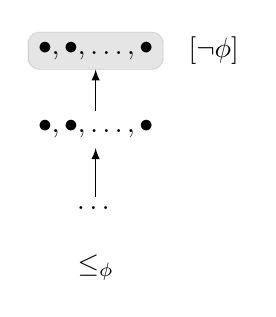
\begin{tikzpicture}
		\node at (0,-0.75){$\le_\phi$};
		\node at (1.5,2){$[\lnot\phi]$};
		\node at (0,2)(0){$\bullet,\bullet,\dots,\bullet$};
		\node at (0,1)(1){$\bullet,\bullet,\dots,\bullet$};
		\node at (0,0)(2){\dots};
		\path[-latex] (2) edge (1)(1) edge (0);
		\fill[draw, opacity=0.1, rounded corners=4]
			(0.south)--
			(0.south west)--
			(0.west)--
			(0.north west)--
			(0.north)--
			(0.north east)--
			(0.east)--
			(0.south east)--
			(0.south);
	\end{tikzpicture}
	\caption{
		A schematic depiction of a total preorder $\le_{\phi}$ 
		in an e-faithful assignment.
		As usual, bullets stand for interpretations.
		Models of $\lnot\phi$ (i.e., interpretations not satisfying $\phi$)
		are shaded in gray. 
	}
	\label{fig:3-enforcement-efaithful-schematic}
\end{figure}

To fix notation, an $\L$-assignment $\as$ on interpretations
is \emph{e-faithful} if it satisfies properties $\ooe{5-6}$.
A schematic depiction of a preorder in an e-faithful 
assignment is given in Figure \ref{fig:3-enforcement-efaithful-schematic}.
Note that the models of $\lnot\phi$ are at the very top.


\subsubsection{Enforcement as choice over outcomes}
The next step in modeling enforcement as a choice procedure
is to link up enforcement as an operation on formulas satisfying 
postulates $\ppe{1-6}$ 
to plausibility relations satisfying properties $\ooe{1-6}$.
This is achieved via a choice procedure, 
which in the case of revision and update amounts to picking 
the best outcomes from the models of the newly acquired 
information $\mu$, 
in effect removing models of $\mu$ that are not optimal. 
However, the nature of the enforcement postulates points 
to a choice procedure that is in many ways
different from that of revision and update:
instead of removing models from $\mu$,
an enforcement operator wants to add to the models of $\mu$:
ideally, it adds all the models of $\phi$.
But if this is not 
possible (in case $\phi\lor\mu$ is a tautology),
some models of $\phi$ will have to be discarded.
This is still an optimization-focused behavior, 
but the parameters under which it functions are new:
using a plausibility ranking on interpretations
in this setting 
becomes a question of not which outcomes are 
more readily held on to,
but which are more readily given up:
a small, but, as we will see, important distinction.

To characterize enforcement we introduce a new way 
of choosing based on a total preorder $\le_{\phi}$ on interpretations.
This method uses the preorder $\le_{\phi}$
to incrementally add interpretations to $[\mu]$,
until further addition becomes impossible.
Thus, if $\W$ is a set of interpretations and 
$\le$ is a preorder on interpretations,
then, for $i\geq 1$, the 
\emph{best-to-worst $\le$-level $i$ of $\W$}, denoted $\lvl_\le^i(\W)$,
is defined by taking:
\begin{align*}
\lvl_\le^1(\W) &= \min_\le(\W),\\
\lvl_\le^{i+1}(\W) &= \min_\le(\W\setminus(\lvl^1_{\le}(\W)\cup\dots\cup\lvl_\le^i(\W))).
\end{align*}
The intuition is that the elements on 
level $i$ are the $i^\text{th}$ best elements of $\W$,
according to $\le$:
we intend to construct the set of models of $\phi \en \mu$
iteratively,
by adding interpretations to $\mu$ in successive steps,
and the $\le$-levels of $\W$ will provide the order 
in which to do so.
It is straightforward to see that 
the best-to-worst levels form a partition of the set $\W$.

Next, we must specify how to actually
construct $[\phi \en \mu]$.
If $\W$ is a set of interpretations, 
the \emph{addition operator $\add^i_{\le}(\W)$} is defined,
for $i\ge 1$, as follows:
\begin{align*}
\add_\le^1(\W) &=\W,\\
\add_\le^{i}(\W) &= 
\begin{cases}
\add_\le^{i-1}(\W)\cup\lvl_{\le}^{i-1}(\U\setminus\W),~\text{if}~\add_\le^{i-1}(\W)\cup\lvl_{\le}^{i-1}(\U\setminus\W)\neq\U,\\
\add_\le^{i-1}(\W),~\text{otherwise}.
\end{cases}
\end{align*}

Intuitively, the addition operator starts from $\W$
and iteratively adds interpretations that are not already in $\W$,
in the order prescribed by $\le_\phi$.
Addition of new interpretations is 
controlled by an acceptance condition,
saying that the new result should not be a tautology.
If the acceptance condition is satisfied then the 
interpretations under considerations 
are added and the operator moves on
to the next level; if not, the operator 
falls back to the result obtained at the previous level.
The starting point guarantees that $\W$ 
is included in $\add_\le^{i}(\W)$, for $i\ge 0$.
Note that, since $\W$ is finite and $\le$ is a total preorder, 
this operation also reaches a fixed point,
i.e., there exists an $i\in\mathbb{\W}$ such that
$\add^j_\le(\W)=\add^i_\le(\W)$, for any $j>i$.
Thus, if 
$\W$ is a set of interpretations and $\le$
is a total preorder on $\W$,
then
\emph{the fixed point of the operator $\add$} is denoted by
$\add_\le^\ast(\W)$.

With the notion of the addition operator in hand,
we can now define a choice procedure that exploits 
a total preorder on interpretations to yield 
the result of enforcing $\mu$ with respect to $\phi$.
Thus, if $\as$ is a total, syntax insensitive and e-faithful
assignment, 
the \emph{$\as$-induced $\L$-enforcement operator $\en^\as$} is defined,
for any propositional formulas $\phi $ and $\mu$,
as follows:
$$
[\phi\en^\as\mu]\defeq\add^\ast_{\le_\phi}[\mu].
$$

Conversely, we want to use an $\L$-enforcement operator $\en$
to infer a ranking over interpretations,
under the assumption that choice is made using the iterative approach
described above.
For revision and update, we would do this using the $\L$-proxy 
of a pair of interpretations $w_1$ and $w_2$, 
i.e., a propositional formula $\px_{1,2}$
such that $[\px_{1,2}]=\{w_1,w_2\}$,
to ask the agent which of the two outcomes it 
wants to hold on to.
Enforcement, which, as we have seen, 
is a kind of dual of revision,
requires a different tactic: 
we will use the $\L$-antiproxy
of a pair of interpretations $w_1$ and $w_2$,
i.e., a propositional formula 
$\px_{-1,-2}$ such that $[\px_{-1,-2}]=\U\setminus\{w_1,w_2\}$,
to ask the agent which of the two outcomes it wants to
give up.
Then, 
if $\en$ is an enforcement operator,
the \emph{$\en$-revealed relation $\le_\phi$} is defined by taking,
for any interpretations $w_1$ and $w_2$:
$$
	w_1\le^{\en}_\phi w_2~\text{if}~w_2\notin[\phi\en\px_{-1,-2}].
$$
The rationale here is that $w_2$ is 
less preferred than $w_1$ if it is more readily given up:
since the rules of enforcement say that 
${\px_{-1,-2}}\subseteq [\phi\en \px_{-1,-2}]\subset\U$,
interpretations $w_1$ and $w_2$ cannot both 
be added to $\phi \en \px_{-1,-2}$
so a choice must be as to which to give up.
If $w_2$, rather than $w_1$, is given up, this indicates that
$w_1$ is preferred to $w_2$; giving both of them up means that
they are equally preferred. 

\begin{figure}\centering
	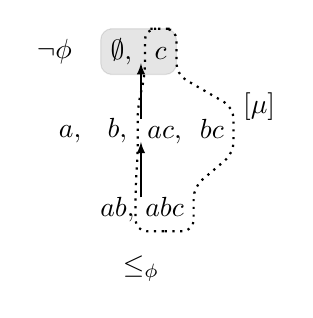
\begin{tikzpicture}
		\node at (0,-0.75){$\le_\phi$};

		\node at (-0.3,0)(ab){$ab,$};
		\node at (0.3,0)(abc){$abc\vphantom{,}$};
		\node[inner sep=0.4em] at (0,0)(a1){};
	
		\node at (-0.9,1)(a){$\vphantom{b,}a,$};	
		\node at (-0.3,1)(b){$b,$};		
		\node at (0.3,1)(ac){$\vphantom{\emptyset}ac,$};
		\node at (0.9,1)(bc){$bc\vphantom{\emptyset,}$};
		\node[inner sep=0.4em] at (0,1)(a2){};

		\node at (-0.25,2)(e){$\emptyset,$};
		\node at (0.25,2)(c){$\vphantom{\emptyset,}c$};
		\node[inner sep=0.4em] at (0,2)(a3){};

		\node at (-1.1,2){$\mods{\lnot\phi}$};
		\node at (1.5,1.3){$[\mu]$};
	
		\path[-latex] (a1) edge (a2)(a2)edge(a3);
		
		\fill[draw, opacity=0.1, rounded corners=4]
			(c.south)--
			(e.south)--
			(e.south west)--
			(e.west)--
			(e.north west)--
			(e.north)--
			(c.north)--
			(c.north east)--
			(c.east)--
			(c.south east)--
			(c.south);
		\draw[thick, dotted, rounded corners=4]
			(abc.south)--
			(abc.south east)--
			(abc.east)--
			(abc.north east)--
			(bc.south east)--
			(bc.east)--
			(bc.north east)--
			(c.south east)--
			(c.east)--
			(c.north east)--
			(c.north)--
			(c.north west)--
			(c.west)--
			(c.south west)--
			(ac.north west)--
			(ac.west)--
			(ac.south west)--
			(abc.north west)--
			(abc.west)--
			(abc.south west)--
			(abc.south);
	\end{tikzpicture}
	\caption{
		A total preorder $\le_{\phi}$ assigned to $\phi$,
		with $[\phi]=\{a,b,ab,ac,bc,abc\}$,
		by a total, syntax insensitive and e-faithful 
		assignment.
		Note that the interpretations not satisfying $\phi$,
		i.e., models of $[\lnot\phi]$,
		are the least preferred outcomes in this preorder
		and are in the gray region.
		The new information is $\mu$,
		with $[\mu]=\{c,ac,bc,abc\}$.
		Enforcing $\mu$ with respect to $\phi$ involves adding 
		interpretations to $[\mu]$ that are not already in 
		$[\mu]$ in the order prescribed by $\le_{\phi}$,
		unless a tautology is created.
	}
	\label{fig:3-enforcement-preorder-operator-interaction}
\end{figure}	

\begin{xmpl}{The art of diagnosis, using a preorder on outcomes}{3-enforcement-preorder-operator-interaction}
	For the setting in Example \ref{ex:3-enforcement-basic-setup},
	with $\phi=a\lor b$ and $\mu=c$, 
	we have that $[\phi]=\{a,b,ab,ac,bc,abc\}$ and $[\mu]=\{c,ac,bc,abc\}$.
	Consider, first, a total, syntax independent $\L$-assignment $\as$ on interpretations
	that assigns to $\phi$ the preorder $\le_{\phi}$
	in Figure \ref{ex:3-enforcement-preorder-operator-interaction}.
	We obtain $[\phi \en \mu]$ by applying the addition operator $\add$
	to $[\mu]$.
	The addition operator starts from $[\mu]$ 
	and takes the levels of ${\lnot\mu}$ in order, trying to add them
	to $\mu$ while avoiding the creation of a tautology. 
	The operation is successful for the first and second levels, after which
	a fixed point is reached.
	The result is:
	\begin{align*}
		[\phi\en\mu] &=\add^\ast_{\le_\phi}[\mu]\\
					 &=([\mu]\cup\{ab\})\cup \{a,b\}\\
					 &=\{a,b,c,ab,ac,bc,abc\}.
	\end{align*}
	Converting the result back into a propositional formula,
	we obtain that $\phi\en\mu\equiv a\lor b\lor c$.

	Conversely, the ranking between two outcomes, 
	say $a$ and $ab$, 
	relative 
	to the prior information $\phi$, with $[\phi]=\{a,b,ab,ac,bc,abc\}$,
	can be elicited by asking the agent 
	to enforce the new information $\px_{-1,-2}$,
	with $[\px_{-1,-2}]=\{\emptyset,b,c,ac,bc,abc\}$.
	Supposing the result is $[\phi\en\px_{-1,-2}]=[\px_{-1,-2}]\cup\{ab\}$,
	we can conclude that, according to the $\en$-revealed ranking,
	it holds that $ab<^{\en}_{\phi}a$.
	This is consistent with $\le_{\phi}$ 
	as depicted in Figure \ref{fig:3-enforcement-preorder-operator-interaction}.
\end{xmpl}

The test of our construction, of course, is whether 
postulates $\ppe{1-6}$, properties $\ooe{1-6}$ and the choice 
procedure formalized by the addition operator $\add$
work together to describe a single belief change mechanism.
The validation comes in the form of a representation theorem,
which shows that these notions cohere with each other.
Before introducing the result, though,
we need to explain what it means for an $\L$-assignment 
$\as$ on interpretations to represent an enforcement operator.
Thus, if $\en$ is an $\L$-enforcement operator 
and $\as$ is an $\L$-assignment on interpretations,
then \emph{$\as$ represents $\en$}
(alternatively, \emph{$\en$ is represented by $\as$})
if, for any propositional formulas $\phi$ and $\mu$,
it holds that $[\phi\en\mu]=\add^\ast_{\le_\phi}[\mu].$
We can now introduce the main representation theorem 
of this section.

\begin{thm}{}{3-enforcement-repr}
	An $\L$-enforcement operator $\en$ 
	satisfies postulates $\ppe{1-6}$ if and only if
	there exists an $\L$-assignment $\as$
	that satisfies properties $\ooe{1-6}$
	(i.e., that is total, syntax insensitive and
	e-faithful)
	and that represents the operator $\en$.
\end{thm}
\begin{prf*}{}{}%
	(``$\Leftarrow$'')
	Note that a preorder $\le_{\phi}$ that satisfies properties 
	$\ooe{1-6}$ can be seen as a preorder $\le_{\lnot\phi}$,
	i.e., a preorder depending on $\lnot\phi$, 
	by taking $w_1\le_{\lnot\phi}w_2$ if $w_2 \le_{\phi}w_1$,
	i.e., by turning $\le_{\phi}$ upside down.
	In this case, $\le_{\lnot\phi}$ satisfies 
	the revision properties $\oor{1-7}$.
	Note that in this setting we have that the complement of 
	$\add^\ast_{\le_\phi}[\mu]$ consists of the minimal 
	models of $\lnot\mu$ in the preorder $\lnot\phi$ as just 
	defined. We can now see that the upside down assignment 
	corresponds to a total, syntax insensitive r-faithful assignment,
	which corresponds to a revision operator $\re$ that 
	satisfies postulates $\ppr{1-6}$.
	Furthermore, we get that 
	$[\phi\en\mu]=\U\setminus(\lnot\phi\re\lnot\mu)$,
	which, by Proposition \ref{prop:3-enforcement-duality},
	implies that $\en$ satisfies postulates $\ppe{1-6}$.

	(``$\Rightarrow$'')
	The $\en$-revealed assignment is the assignment we are looking for,
	and it is straightforward to check that it satisfies properties $\ooe{1-6}$
	and that it represents the operator $\en$.
\end{prf*}

A quick note is in order on previous results.
Existing work on propositional enforcement \cite{HaretWW18} 
has used partial orders 
on sets of interpretations (or, alternatively, on formulas)
to represent enforcement operators, 
but a nice representation in terms of preorders on interpretations themselves, 
\`a la Theorem \ref{thm:3-revision-repr-km-total}, was left open.
Here we filled this gap.
Note, also, that a representation in terms of preorder on interpretations
can be obtained in a more naive way, by using 
Equations \ref{eq:revision-to-enforcement} 
and \ref{eq:enforcement-to-revision} 
and Theorem \ref{thm:3-revision-repr-total}.
Thus, given an enforcement operator $\en$ 
satisfying postulates $\ppe{1-6}$, 
we can immediately infer that there exists 
an $\L$-assignment $\as$ on interpretations
that satisfies properties $\oor{1-5}$ and $\oor{7}$ 
such that, for any propositional formulas $\phi$ and $\mu$, 
the following holds:
$$
	[\phi\en\mu] = [\lnot(\lnot\phi\re^\en\lnot\mu)]=\U\setminus\min_{\le_{\lnot\phi}}[\lnot\mu].
$$
In other words, we can use an assignment representing 
the $\en$-induced $\L$-revision operator $\re^\en$ to represent $\en$.
However, this expression is not very informative and, 
as we have shown, unnecessarily circuitous.

\subsubsection{Distance-based enforcement operators}
Theorem \ref{thm:3-enforcement-repr} offers some insight 
into how to construct concrete enforcement operators:
find a way to generate e-faithful assignments, 
i.e., preorders on interpretations in which the top elements 
are the non-models of $\phi$.
It turns out that the tried and tested methods of 
quasi-distances between interpretations
and aggregation functions 
used in revision and update work here as well, with minimal adjustment.

We bring up aggregation functions only to settle straight away 
that the only aggregation function we will use in this section 
is the $\min$ aggregation function: we will be using it, however,
in a slightly different way than in revision.
For the next definition, recall that the size of the set $\Atoms$
is assumed to be $m$.
If $\dd$ is a quasi-distance between interpretations,
$\phi$ is a propositional formula and $w$ is an interpretation,
then the 
\emph{$(\dd,\:m-\min)$-induced distance $\dd^{m-\min}(\phi,w)$ between $\phi$ and $w$} 
is defined as:
$$
	\dd^{m-\min}(\phi,w) = m-\min(\dd(v,w))_{v\in[\phi]}.
$$
Intuitively, $\dd^{m-\min}(\phi,w)$ can be thought of as the inverse
of the more familiar notion $\dd^{\min}(\phi,w)$ 
(see Sections \ref{sec:2-distances} or \ref{sec:3-revision}):
a penalty is introduced for $w$ the closer it is to the models of $\phi$,
such that the interpretations closest to $\phi$ end up receiving the 
highest score
and the interpretations furthest to $\phi$ receive the lowest score,
i.e., $\phi$ is such that it is better to be far away from it than close to it.

Following up, the \emph{$(\dd,\:m-\min)$-induced ranking $\le^{\dd,\:m-\min}_{\phi}$}
is defined as:
$$
	w_1\le^{\dd,\:m-\min}_\phi w_2~\text{if}~\dd^{m-\min}(\lnot\phi,w_1)\le\dd^{m-\min}(\lnot\phi,w_2).
$$
What we are saying, in effect, is that $w_1$ is preferred to $w_2$ relative to $\phi$,
according to $\le^{\dd,\:m-\min}_{\phi}$ if $w_1$ is farther away from $\lnot\phi$ than $w_2$.
If $\dd$ is a quasi-distance,
the \emph{${(\dd,\:m-\min)}$-induced assignment $\as^{\dd,\:m-\min}$} is obtained by taking 
$\as^{\dd,\:m-\min}\!\!(\phi)=\le_\phi^{\dd,\:m-\min}$,
for any propositional formula $\phi$.
In the same vein, the \emph{${(\dd,\:m-\min)}$-induced $\L$-enforcement operator $\en^{\dd,\:m-\min}$} 
is the operator induced by the assignment $\as^{\dd,\:m-\min}$.
This allows us to generate total, syntax insensitive e-faithful assignments.

\begin{prp}{}{3-enforcement-d-induced-preorder}
	If $\dd$ is a quasi-distance between interpretations and $\phi$ is a propositional formula, 
	the ${(\dd,\:m-\min)}$-induced ranking $\le^{\dd,\:m-\min}_\phi$ 
	satisfies properties $\ooe{1-6}$, 
	i.e., $\le^{\dd,\:m-\min}_\phi$ is a total preorder 
	on interpretations that	is syntax insensitive and 
	makes the models of $\lnot\phi$ the 
	$\le^{\dd,\:m-\min}_\phi$-maximal elements.
\end{prp}
\begin{prf*}{}{}%
	It is straightforward to see that $\le_{\phi}^{\dd,\:m-\min}$ 
	is a total preorder on interpretations,
	i.e., that $\le_{\phi}^{\dd,\:\min}$ satisfies properties $\ooe{1-3}$.
	Since the definition of $\le_{\phi}^{\dd,\:m-\min}$ 
	depends only on the interpretations,
	$\le_{\phi}^{\dd,\:m-\min}$ also satisfies property $\ooe{4}$.
	Finally, it holds that:
	$\dd^{m-\min}(\lnot\phi,w) = m- \min(\dd(v,w))_{v\in[\lnot\phi]} = m$ if and only if
	$w\in[\lnot\phi]$, 
	which implies that models of $\lnot\phi$ are the $\le_{\phi}^{\dd,\:m-\min}$-maximal
	elements in $\le_{\phi}^{\dd,\:m-\min}$,
	i.e., $\le_{\phi}^{\dd,\:m-\min}$ satisfies 
	properties $\ooe{5}$ and $\ooe{6}$, 
	for any propositional formula $\phi$.		
\end{prf*}

Proposition \ref{prop:3-enforcement-d-induced-preorder} 
implies that the $({\dd,\:m-\min})$-induced assignment $\as^{\dd,\:m-\min}$ 
is total, e-faithful and syntax insensitive, 
which, by Theorem \ref{thm:3-enforcement-repr}, 
implies that the $({\dd,\:m-\min})$-induced $\L$-enforcement operator 
$\en^{\dd,\:\min}$ satisfies postulates $\ppe{1-6}$.

\begin{crl}{}{3-enforcement-d-induced-operator}
	If $\dd$ is a quasi-distance between interpretations, 
	the $(\dd,\:m-\min)$-induced $\L$-enforcement 
	operator $\en^{\dd,\:m-\min}$ 
	satisfies postulates $\ppe{1-6}$.
\end{crl}

As examples of concrete distances we can use the Hamming distance $\dd_{\hamming}$
and the drastic distance $\dd_{\drastic}$, giving rise to the $\L$-enforcement operators 
$\en^{\hamming,\:m-\min}$ and $\en^{\drastic,\:m-\min}$.

\begin{figure}\centering
	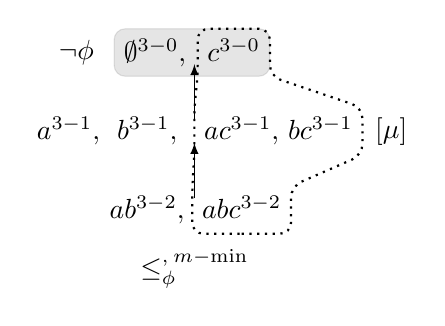
\begin{tikzpicture}
		\node at (0,-0.75){$\le^{\hamming,\:m-\min}_\phi$};

		\node at (-0.6,0)(ab){$ab^{3-2},$};
		\node at (0.6,0)(abc){$abc^{3-2}\vphantom{,}$};
		\node[inner sep=0.4em] at (0,0)(a1){};
	
		\node at (-1.6,1)(a){$\vphantom{b,}a^{3-1},$};	
		\node at (-0.6,1)(b){$b^{3-1},$};		
		\node at (0.6,1)(ac){$\vphantom{\emptyset}ac^{3-1},$};
		\node at (1.6,1)(bc){$bc^{3-1}\vphantom{\emptyset,}$};
		\node[inner sep=0.4em] at (0,1)(a2){};

		\node at (-0.5,2)(e){$\emptyset^{3-0},$};
		\node at (0.5,2)(c){$\vphantom{\emptyset,}c^{3-0}$};
		\node[inner sep=0.4em] at (0,2)(a3){};

		\node at (-1.5,2){$\mods{\lnot\phi}$};
		\node at (2.5,1){$[\mu]$};
	
		\path[-latex] (a1) edge (a2)(a2)edge(a3);
		
		\fill[draw, opacity=0.1, rounded corners=4]
			(c.south)--
			(e.south)--
			(e.south west)--
			(e.west)--
			(e.north west)--
			(e.north)--
			(c.north)--
			(c.north east)--
			(c.east)--
			(c.south east)--
			(c.south);
		\draw[thick, dotted, rounded corners=4]
			(abc.south)--
			(abc.south east)--
			(abc.east)--
			(abc.north east)--
			(bc.south east)--
			(bc.east)--
			(bc.north east)--
			(c.south east)--
			(c.east)--
			(c.north east)--
			(c.north)--
			(c.north west)--
			(c.west)--
			(c.south west)--
			(ac.north west)--
			(ac.west)--
			(ac.south west)--
			(abc.north west)--
			(abc.west)--
			(abc.south west)--
			(abc.south);
	\end{tikzpicture}
	\caption{
		The preorder $\le^{\hamming,\:m-\min}_{\phi}$ 
		assigned to $\phi$,
		with $[\phi]=\{a,b,ab,ac,bc,abc\}$,
		by the $\as^{\hamming,\:m-\min}$ 
		assignment.
		The superscripts denote the distance to $\lnot\phi$
		subtracted from the number of atoms in $\Atoms$,
		which in this case is $3$.
		Note that the interpretations not satisfying $\phi$,
		i.e., models of $[\lnot\phi]$,
		get a score of $3$,
		which makes them the least 
		preferred outcomes.
	}
	\label{fig:3-enforcement-hamming-op}
\end{figure}	

\begin{xmpl}{The art of diagnosis, using distances}{3-enforcement-hamming-op}
	For the setting in Example \ref{ex:3-enforcement-basic-setup},
	with 
	$\Atoms=\{a,b,c\}$,
	$\phi=a\lor b$ and $\mu=c$, 
	the $\L$-assignment $\as^{\hamming,\:m-\min}$ 
	generates the preorder $\le^{\hamming,\:m-\min}_{\phi}$  
	in Figure \ref{fig:3-enforcement-hamming-op}.
	Note that $\le^{\hamming,\:m-\min}_{\phi}$ is the same
	as the preorder $\le_{\phi}$ in Figure \ref{fig:3-enforcement-preorder-operator-interaction}.
	We obtain, as before, that $[\phi\en\mu]=\add^{\ast}_{\le_{\phi}}[\mu]=\{a,b,c,ab,ac,bc,abc\}$.
\end{xmpl}























\section{Merging}\label{sec:3-merging}
If agents deliberate with respect 
to a small number of independent alternatives, 
as is the case in a typical election, 
aggregation of different viewpoints 
is well understood due to existing research 
in the field of social choice \cite{Zwicker16,BaumeisterR16}.
But if agents have to decide on multiple 
interconnected issues at the same time,
then the number of possible alternatives 
can grow too large to expect agents 
to have explicit preferences over the whole set.
We have encountered this kind of scenario 
in Example \ref{ex:1-merging-motivation},
where we have been introduced to four 
Academy members trying to decide who will 
be the nominees in this year's \emph{Best Director} category.

\begin{xmpl}{$\#$OscarsSoFossilized}{3-merging-basic-setup}
	In Example \ref{ex:1-merging-motivation}
	the names being circulated are Alma Har'el, Bong Joon Ho and C\'eline Sciamma,
	represented by propositional variables
	$a$, $b$ and $c$, respectively.
	The decision as to who will be the nominees
	is left up to four Academy members.
	Each of the four members has their own opinion 
	about who should be nominated, represented by propositional formulas 
	$\phi_1 = a\land b$,
	$\phi_2 = a\land (b\lor c)$,
	$\phi_3 = \lnot a\land b \land \lnot c$.
	and
	$\phi_4 = \lnot a \land\lnot b\land c$.
	The final lineup should consist of only two people,
	i.e., the individual opinions should be aggregated subject to the constraint
	$\mu=(a\land b\land \lnot c)\lor (a\land\lnot b\land c)\lor(\lnot a\land b\land c)$.
	These opinions are collectively inconsistent, 
	but none of them weighs more than the others.
\end{xmpl}

In Example \ref{ex:3-merging-basic-setup},
a standard social choice procedure would require
the Academy members to provide a ranking 
of all the possible lists of two nominees, 
or, as we code them here, of the outcomes 
$ab$, $bc$, $ac$.
Though this would not be too difficult for this example,
the cognitive burden on the agents will certainly become too big
if the number of possibilities or the size of the lineup 
grew even slightly. 
This is certain to be the case even for the Oscars:
Example \ref{ex:3-merging-basic-setup} is only a toy example,
since the real world list of \emph{Best Director} nominees is 
usually made up of five people, and the list of possible 
nominees is much larger. 
In the real world scenario, asking Academy members to rank all possible
combinations of five directors is clearly unfeasible.

This problem, known more generally as \emph{combinatorial voting} \cite{LangX16}, 
acquires a knowledge representation dimension 
as agents need compact ways to express their positions over 
a large domain, and automatizable procedures 
to perform reasoning with such positions.
Merging, in this context, can prove useful,
as it provides a versatile framework in which different agents 
can combine their positions on a fixed set of issues,
expressed as propositional formulas,
into a collective perspective, expressed, likewise,
as a propositional formula \cite{KoniecznyP02,KoniecznyP11}.

In Example \ref{ex:3-merging-basic-setup}
a merging operator should combine the information 
provided by the four Academy members
while making sure that the cardinality constraint $\mu$ is satisfied.
What the theory of belief merging offers is
a core set of postulates to assess the rationality of any merging operator,
and a range of concrete operators tailored according to these principles.
Seeing merging operators as a type of collective decision procedure
is a natural interpretation of the process:
the propositional atoms in the alphabet can be taken 
to encode issues that are deliberated upon,
while truth-value assignments to atoms, 
i.e., the interpretations or outcomes, 
encode combinations of issues that could make it 
into the final result, and over which agents can have preferences.
The propositional formulas submitted by agents 
represent the way in which issues are interconnected in the agents' preferences,
and the result is a set of ``winning'' interpretations,
representable as a propositional formula, 
that respect the integrity constraint of the merging process. 

\subsubsection{Postulates}
An \emph{$\L^{n}$-merging operator $\me$} 
is a function $\me\colon\L^n\rightarrow\L$,
taking as input 
a propositional profile $\P=(\phi_i)_{1\le i \le n}$
and a propositional formula $\mu$,
and returning a propositional formula, 
denoted by $\me_\mu(\P)$.
In the context of merging the formula $\mu$,
which we normally call the new information,
is called an \emph{integrity constraint}.
Merging is a multi-agent operation,
in the sense that the formulas in a profile $\P$
originate with different agents, 
usually gathered in the set $N=\{1,\dots,n\}$,
with formula $\phi_{i}$ corresponding to agent $i$.

The following postulates are typically taken to provide a core set of rationality constraints
any merging operator $\me$ is expected to satisfy.
They are expected to hold for any propositional profiles $\P$, $\P_1$, $\P_2$,
formulas $\phi_1$, $\phi_2$
and constraints $\mu$, $\mu_{1}$ and $\mu_{2}$:

\begin{description}
	\item[($\ppm{0}$)] $\me_\mu(\P)\models\mu$.
	\item[($\ppm{1}$)] If $\mu$ is consistent, then $\me_\mu(\P)$ is consistent.
	\item[($\ppm{2}$)] If $\bigwedge\P\land\mu$ is consistent, then $\me_\mu(\P)\equiv\bigwedge\P\land\mu$.
	\item[($\ppm{3}$)] If $\P_1\equiv \P_2$ and $\mu_1\equiv\mu_2$, 
	then $\me_{\mu_1}(\P_1)\equiv\me_{\mu_1}(\P_2)$.
	\item[($\ppm{4}$)] If $\phi_1\models\mu$ and $\phi_2\models\mu$, 
	then $\me_\mu(\phi_1,\phi_2)\land\phi_1$ is 
	consistent if and only if $\me_\mu(\phi_1,\phi_2)\land\phi_2$ is consistent.
	\item[($\ppm{5}$)] $\me_\mu(\P_1)\land\me_\mu(\P_2)\models\me_\mu(\append{\P_1}{\P_2})$.
	\item[($\ppm{6}$)] If $\me_\mu(\P_1)\land\me_\mu(\P_2)$ is consistent, then 
	$\me_\mu(\append{\P_1}{\P_2})\models\me_\mu(\P_1)\land\me_\mu(\P_2)$.
	\item[($\ppm{7}$)] $\me_{\mu_1}(\P)\land\mu_2\models\me_{\mu_1\land\mu_2}(\P)$.
	\item[($\ppm{8}$)] If $\me_{\mu_1}(\P)\land\mu_2$ is consistent, then
	$\me_{\mu_1\land\mu_2}(\P)\models\me_{\mu_1}(\P)\land\mu_2$.
\end{description}

Postulate $\ppm{0}$ says that the merging result $\me_{\mu}(\P)$ should
satisfy the constraint $\mu$.
Postulate $\ppm{1}$ says that the result 
should be consistent if $\mu$ is consistent.
Postulate $\ppm{2}$ requires that if there 
is any agreement between the formulas in $\P$ and $\mu$,
then the merged result is nothing more than the agreed upon outcomes.
Postulate $\ppm{3}$ says that the result 
should be insensitive to the syntax of the formulas involved.
Postulate $\ppm{4}$ stipulates that merging two formulas $\phi_1$ and $\phi_2$ should be fair,
in the sense that if the result contains outcomes consistent with one of the formulas, it should contain 
results consistent with the other as well.
Postulates $\ppm{5-6}$ say that the result should
include outcomes that are unanimously accepted across subprofiles.
Postulates $\ppm{7-8}$ say that the result 
and coherent when varying the constraint.

Though postulates $\ppm{0-8}$ are referred to here using our custom naming convention,
in the literature they are more commonly known as the $IC$-postulates \cite{KoniecznyP02,KoniecznyP11},
where `$IC$' stands for \emph{integrity constraint} and indicates that merging is done within the purview of 
the condition $\mu$, which must be satisfied by the merging result $\me_\mu(\P)$.

Note that, insofar as a profile $\P=(\phi_i)_{1\le i \le n}$ 
is identified with the single propositional 
formula $\bigwedge_{\phi_i\in\P}\phi_{i}$, 
then postulates $\ppm{0-3}$ and $\ppm{7-8}$ correspond to revision postulates
$\ppr{1-4}$ and $\ppr{5-6}$, respectively,
where $\bigwedge\P$ is the prior belief and $\mu$ is the newly acquired information.
Thus, another way of looking at a merging operator $\me$ 
is to see it as a revision operator that needs to satisfy some additional
properties, besides the standard ones presented in Section \ref{sec:3-revision}.
These properties are postulates $\ppm{4-6}$, and what they add 
is the notion that the formulas that go into the prior belief (or rather, their models)
should carry equal weight in the change process. 
This corresponds to the idea that merging is a public, 
or social operation, whose participants should be treated fairly.
Consequently, postulates $\ppm{0-8}$ are best understood as axiomatizing a decision procedure 
based on the aggregation of information coming from different sources, i.e., the formulas in $\P$.

\begin{xmpl}{Possible Oscar nominees}{3-merging-postulates}
	For the merging scenario in Example \ref{ex:3-merging-basic-setup}
	the profile is $\P=(\phi_1,\phi_2,\phi_3,\phi_4)$,
	where 
	$\phi_1 = a\land b$,
	$\phi_2 = a\land (b\lor c)$,
	$\phi_3 = \lnot a\land b \land \lnot c$
	and
	$\phi_4 = \lnot a \land\lnot b\land c$.
	Examples \ref{ex:1-merging-motivation} 
	and \ref{ex:3-merging-basic-setup} provide the meaning
	for these formulas.
	The constraint is represented by the propositional formula
	$\mu=(a\land b\land \lnot c)\lor (a\land\lnot b\land c)\lor(\lnot a\land b\land c)$,
	with $[\mu]=\{ab,bc,ac\}$.


	Suppose that $\me$ is a merging operator that satisfies postulates $\ppm{0-8}$
	and $\me_\mu(\P)\equiv (a\land b)\lor(b\land c)$,
	i.e., $[\me_\mu(\P)]=\{ab,bc\}$. This result is in line with 
	postulate $\ppm{1}$ (i.e., it is consistent)
	and	with postulate $\ppm{0}$ (i.e., implies $\mu$).
	The models of $[\me_\mu(\P)]$ encode the makeup of the list of nominees,
	e.g., $ab$ means that Alma Har'el and Bong Joon Ho (but not C\'eline Sciamma) will be nominated.
\end{xmpl}

As with revision and the other belief change operations we 
have looked at in this chapter, 
the positions of the agents could be beliefs, intentions or simply 
combinations of issues that agents find desirable, 
and would like to see in the result.
The consistent insistence on insensitivity to syntax means that 
the propositional formulas that stand for the agents' positions 
are, in a sense, just window dressing for their models.
This is another way of saying that
belief change operations are interested more in the underlying issues 
rather than in how they are expressed.
Of course, the representation may matter for cognitive or computational 
purposes, but for the belief change operators we consider here 
the formulas are just compact representations of sets of outcomes the agents 
are interested in.
Thus, whether or not the formulas encode (actual) beliefs is not of 
immediate crucial importance to a merging operator:
postulates $\ppm{0-8}$ are neutral with respect to the cognitive attitude
being expressed.

That being said, the exact meaning of the formulas \emph{will} matter 
if we want to be more specific about the type of information aggregation a belief merging 
operator performs. Thus, there is a significant difference between aggregating 
bits of information the agents believe are true, when there is, actually,
a true state of the world,
versus aggregating sets of issues the agent want to see obtain,
in which case there might not be a true answer at all.
In the former case the purpose of a merging operator is to track the truth,
whereas in the latter case the purpose of a merging operator is to be fair 
towards the participants.
Correspondingly, the criteria a merging operator is expected to satisfy 
will be different depending on the kind of task it is used for:
a truth-tracking operator will be expected to be accurate, 
whereas a fair merging operator will be expected to be impartial 
towards the agents, strategyproof or proportional.

In this work we are interested in merging more as a tool for collective decision 
making than as a way of aggregating information about the world, 
and will therefore focus on the fairness aspects of merging.
Work on the truth-tracking abilities of merging exists \cite{EveraereKM10},
but is outside the scope of the current work.


\subsubsection{Preferences over outcomes}
In the context of merging, 
preference orders are ushered in 
through an \emph{$\L^{n}$-assignment $\as$ on interpretations}, 
which is a function $\as\colon\L^n\rightarrow 2^{\U\times\U}$ 
that maps $\L$-profiles
to preference orders on interpretations.
In Sections \ref{sec:3-revision} and \ref{sec:3-update}
we have modeled both total and partial preorders,
but here we will work mainly with total preorders.
Since we want to pursue the parallel between 
merging and a collective decision process,
the relation $\le_{\P}$ assigned to a profile 
$\P=(\phi_i)_{1\le i \le n}$
by an $\L^n$-assignment $\as$ on interpretations
can be thought of as the collective ranking, 
obtained by aggregating the preferences of each agent 
in $N=\{1,\dots,n\}$.
In this context, the preferences of the agents themselves 
are given by $\le_{(\phi_{i})}$,
i.e., by the preference associated with the profile $(\phi_{i})$ 
having only $\phi_{i}$ as element.
In the interest of readability, we will generally write 
simply $\le_{\phi_i}$ instead of $\le_{(\phi_i)}$, 
when only one agent is involves.

Under the assumption of an $\L^n$-assignment $\as$ on interpretations,
we have both that the individual preference orders $\le_{\phi_{i}}$, for $i\in N$,
as well as the collective preference $\le_{\P}$, exist.
The purpose of merging, however, is to make sure 
not only that the individual and collective preference 
orders exist, but that they also have desirable properties,
i.e., that the collective preference order can be seen 
to aggregate, in a fair and reasonable way,
the information provided by the individual preference orders.
This is ensured by writing down desirable properties 
of an $\L^n$-assignment $\as$ on interpretations.
The properties an $\L^n$-assignment is expected to satisfy 
include some familiar properties, but also some new ones.
Recall that two propositional profiles $\P_1$ and $\P_2$
are equivalent, written $\P_1\equiv\P_2$, if there is a bijection
$f\colon\P_1\rightarrow\P_2$ such that $f(\phi_i)\equiv \phi_i$,
for any $\phi_i\in\P_1$.
The properties are expected to apply for any propositional profiles 
$\P$, $\P_1$, $\P_2$, propositional formulas $\phi_1$ and $\phi_2$,
and interpretations $w$, $w_1$ and $w_2$:

\begin{description}
	\item[($\oom{1}$)] $w\le_\P w$.
	\item[($\oom{2}$)] If $w_1\le_\P w_2$ and $w_2\le_\P w_3$, then $w_1\le_\P w_3$.
	\item[($\oom{3}$)] $w_1\le_\P w_2$ or $w_2\le_\P w_1$.
	\item[($\oom{4}$)] If $\P_1\equiv\P_2$, then $\le_{\P_1} = \le_{\P_2}$.		
	\item[($\oom{5}$)] If $w_1,w_2\in[\P]$, then $w_1\approx_\P w_2$.
	\item[($\oom{6}$)] If $w_1\in [\P]$ and $w_2\notin [\P]$, then $w_1 <_{\P} w_2$.
	\item[($\oom{7}$)] If $\phi_1$ and $\phi_2$ are consistent and $w_1\in[\phi]$,
		then there exists $w_2\in[\phi_2]$ such that $w_2\le_{(\phi_1,\phi_2)}w_1$. 
	\item[($\oom{8}$)] If $w_1\le_{\P_1} w_2$ and $w_1\le_{\P_2} w_2$, 
		then $w_1\le_{\append{\P_1}{\P_2}} w_2$.
	\item[($\oom{9}$)] If $w_1\le_{\P_1} w_2$ and $w_1<_{\P_2} w_2$, 
		then $w_1<_{\append{\P_1}{\P_2}} w_2$.
\end{description}

Properties $\oom{1-3}$ imply that $\le_{\P}$ is a total preorder on interpretations,
and are identical to revision properties $\oor{1-3}$.
Property $\oom{4}$ expresses syntax insensitivity in the context of merging.
Properties $\oom{5-6}$ say that models of a profile $\P$ are the 
uniquely minimal elements in $\le_{\P}$, 
and are equivalent to revision properties $\oor{5}$ and $\oor{7}$, respectively.
Property $\oom{7}$ says that models of two formulas $\phi_{1}$ and $\phi_{2}$
should be treated equally when merging $\phi_{1}$ and $\phi_{2}$,
in the sense that it should not be the case that some model of $\phi_{1}$
gets chosen while all models of $\phi_{2}$ are left out 
(assuming it is possible to choose models from both $\phi_{1}$ and $\phi_{2}$).
Property $\oom{8}$ says that if $w_{1}$ is considered at least as good as $w_{2}$
according to both profiles $\P_{1}$ and $\P_{2}$, then 
$w_{1}$ is also considered at least as good as $w_{2}$ according to the 
profile $\P_{1}+ \P_{2}$, obtained by concatenating $\P_{1}$ and $\P_{2}$;
in other words, agreement about $w_{1}$ and $w_{2}$ carries over to the 
aggregated result.
Property $\oom{9}$ says that if 
if $w_{1}$ is considered at least as good as $w_{2}$
according to both profiles $\P_{1}$ and $\P_{2}$
and, in addition, 
$w_{1}$ is considered strictly better than $w_{2}$
according to at least one of the profiles $\P_{1}$ and $\P_{2}$,
then $w_{1}$ is considered strictly better than $w_{2}$
according to the 
profile $\P_{1}+ \P_{2}$, obtained by concatenating $\P_{1}$ and $\P_{2}$.

\begin{figure}\centering
	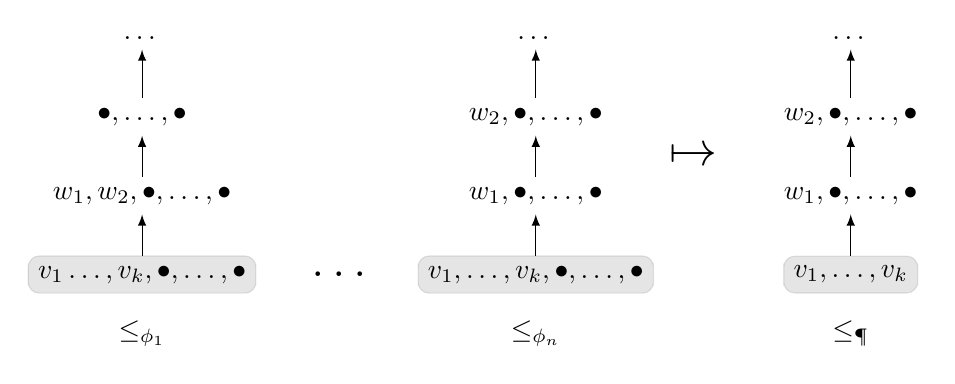
\begin{tikzpicture}
		\node at (0,-0.75){$\le_{\phi_{1}}$};
		\node at (0,0)(0){$v_{1}\dots,v_{k},\bullet,\dots,\bullet$};
		\node at (0,1)(1){$w_1,w_2,\bullet,\dots,\bullet$};
		\node at (0,2)(2){$\bullet,\dots,\bullet$};
		\node at (0,3)(3){\dots};
		\path[-latex] (0) edge (1)(1) edge (2)(2)edge(3);
		\fill[draw, opacity=0.1, rounded corners=4]
			(0.south)--
			(0.south west)--
			(0.west)--
			(0.north west)--
			(0.north)--
			(0.north east)--
			(0.east)--
			(0.south east)--
			(0.south);

		\node at (2.5,0){\LARGE $\dots$};
	
		\node at (5,-0.75){$\le_{\phi_{n}}$};
		\node at (5,0)(0){$v_{1},\dots,v_{k},\bullet,\dots,\bullet$};
		\node at (5,1)(1){$w_1,\bullet,\dots,\bullet$};
		\node at (5,2)(2){$w_2,\bullet,\dots,\bullet$};
		\node at (5,3)(3){\dots};
		\path[-latex] (0) edge (1)(1) edge (2)(2)edge(3);
		\fill[draw, opacity=0.1, rounded corners=4]
			(0.south)--
			(0.south west)--
			(0.west)--
			(0.north west)--
			(0.north)--
			(0.north east)--
			(0.east)--
			(0.south east)--
			(0.south);

		\node at (7,1.5){\LARGE $\mapsto$};

		\node at (9,-0.75){$\le_\P$};
		\node at (9,0)(0){$v_{1},\dots,v_{k}$};
		\node at (9,1)(1){$w_1,\bullet,\dots,\bullet$};
		\node at (9,2)(2){$w_2,\bullet,\dots,\bullet$};
		\node at (9,3)(3){\dots};
		\path[-latex] (0) edge (1)(1) edge (2)(2)edge(3);
		\fill[draw, opacity=0.1, rounded corners=4]
			(0.south)--
			(0.south west)--
			(0.west)--
			(0.north west)--
			(0.north)--
			(0.north east)--
			(0.east)--
			(0.south east)--
			(0.south);
	\end{tikzpicture}
	\caption{
		A schematic depiction of preorders 
		$\le_{\phi_{i}}$, $\le_{\phi_{n}}$ 
		and $\le_{\P}$
		in an m-faithful assignment.
		Bullets stand for interpretations.
		Models of $\phi_{i}$, for $1\le i \le n$,
		and of $\P$
		are shaded in light gray. 
		Note that all agents in 
		$\P$ agree that $w_1$ is at least as good
		as $w_2$ and, in accordance with $\oom{8}$,
		$w_{1}$ is at least as good as $w_2$ in $\le_{\P}$. 
		What is more, in $\le_{\phi_{n}}$ it holds that
		$w_{1}$ is strictly preferred to $w_{2}$,
		and in accordance with $\oom{9}$, 
		$w_1$ is strictly better than $w_2$ in $\le_{\P}$.
		Note, also, that $v_1$, \dots, $v_k$
		are models of every formula in $\P$,
		and are among the minimal elements in each
		preorder $\le_{\phi_{i}}$,
		for $1\le i\le n$. 
		In addition, the models of $\P$,
		i.e., $v_1$, \dots, $v_k$, are the uniquely 
		minimal elements in $\le_{\P}$.
	}
	\label{fig:3-merging-mfaithful-schematic}
\end{figure}

An $\L^n$-assignment $\as$ on interpretations
is \emph{total} if it satisfies properties $\oom{1-3}$,
\emph{syntax insensitive} if it satisfies propery $\oom{4}$
and \emph{m-faithful} if it satisfies properties $\oom{5-9}$.
A total, syntax insensitive and m-faithful assignment 
corresponds to what is
more usually called a \emph{syncretic assignment} \cite{KoniecznyP02,KoniecznyP11}.
A schematic depiction of such an assignment is offered 
in Figure \ref{fig:3-merging-mfaithful-schematic}.

\subsubsection{Merging as social choice over outcomes}
Apart from the multi-agent flavour given by the extra postulates,
merging can be formalized as a bona-fide belief change operator
along the same lines as revision, update and enforcement.
This means using the preference information afforded by an 
$\L^n$-assignment $\as$ on interpretations to obtain the result
of merging formulas in a profile and, conversely, 
using the merging result to infer the underlying preference relation.
Recall, for this, that the $\L$-proxy of a pair $\{w_1,w_2\}$ of interpretations
is a propositional formula $\px_{1,2}$ such that $[\px_{1,2}]=\{w_1,w_2\}$.

Thus, if $\as$ is an $\L^n$-assignment on interpretations,
the \emph{$\as$-induced $\L^n$-merging operator $\me^{\as}$} is defined,
for any profile $\P=(\phi_i)_{1\le i \le n}$
and constraint $\mu$, as:
$$
	[\me_{\mu}(\P)] \defeq \min_{\le_{\P}}[\mu].
$$
Conversely, if $\me$ is a merging operator,
then the \emph{$\me$-revealed relation $\le_{\P}^{\me}$ on interpretations}
is defined, for any
propositional profile $\P$ and interpretations $w_1$ and $w_2$, 
as follows:
$$
	w_1 \le^{\me}_{\P} w_2~\text{if}~w_1\in[\me_{\px_{1,2}}(\P)].
$$
Predictably, the \emph{$\me$-revealed $\L^n$-assignment $\as^{\me}$ on interpretations}
is defined, for any propositional profile $\P$, as $\as^{\me}\!\!(\P)=\le_{\P}$.
If $\me$ is an $\L^n$-merging operator 
and $\as$ is an $\L^n$-assignment on interpretations,
then \emph{$\as$ represents $\me$}
(and, alternatively, \emph{$\me$ is represented by $\as$}),
if, for any $\L$-profile $\P=(\phi_i)_{1\le i \le n}$ 
and constraint $\mu$,
it holds that 
$[\me_{\mu}(\P)] = \min_{\le_{\P}}[\mu]$.
The following classical  representation theorem 
shows that postulates $\ppm{0-8}$ and properties $\oom{1-9}$
fit together into a single choice procedure.

\begin{thm}{\cite{KoniecznyP11}}{3-merging-repr}
	An $\L^n$-merging operator $\me$ satisfies postulates $\ppm{0-8}$
	if and only if
	there exists an $\L^n$-assignment $\as$ on interpretations
	that satisfies properties $\oom{1-9}$
	(i.e., is total, syntax insensitive and m-faithful)
	and that represents the operator $\me$.
\end{thm}

As for revision, postulate $\ppm{2}$ enjoys a one-to-one correspondence with 
properties $\oom{5-6}$ and can be separated from the rest of the postulates,
though there is no pressing need to do so for merging operators, 
since we will not consider alternatives to it.

Theorem \ref{thm:3-merging-repr} validates the choice perspective 
as applied to merging operators. According to it a merging 
operator that satisfies postulates $\ppm{0-8}$ 
can be seen as a social choice function as described 
in Section \ref{sec:2-choice-functions}, with a preference profile, 
an aggregation rule and a set of winner.
The preference profile is $(\le_{\phi_{i}})_{1\le i \le n}$,
i.e., it is made up of the individual preference orders 
of every agent in $\P$, guaranteed to exist in the assignment
that represents $\me$.
The merging operator is the aggregation function, and the set of winners 
are the models of $\me_{\mu}(\P)$.
In fact, under the assumption of an $\L^n$-assignment $\as$ on interpretations,
the merging operator $\me$ is even a social welfare function, since the result
is actually a preorder, i.e., the preorder $\le_{\P}$ associated to $\P$.


\begin{figure}
	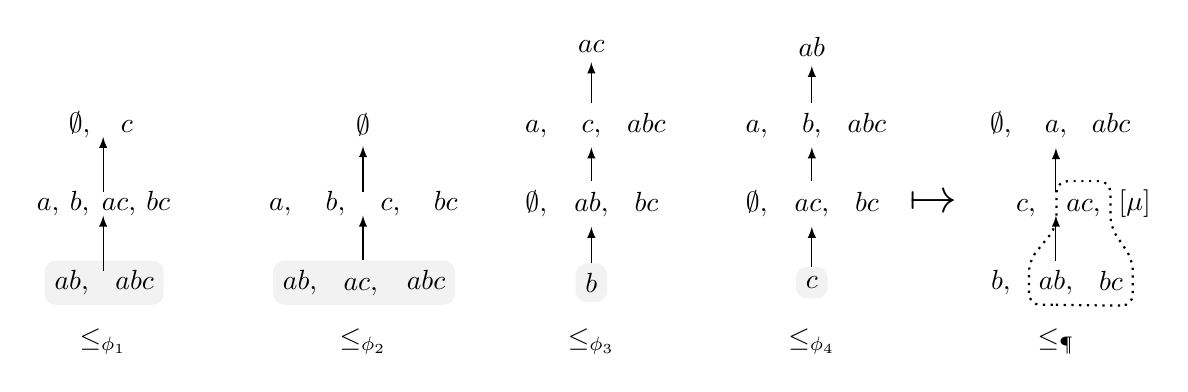
\begin{tikzpicture}
		%% phi1
		\node at (0,-0.75){$\le_{\phi_1}$};

		\node at (-0.4,0)(ab){$ab,$};
		\node at (0.4,0)(abc){$abc\vphantom{,}$};
		\node[inner sep=0.4em] at (0,0)(a1){};
	
		\node at (-0.7,1)(a){$\vphantom{b,}a,$};	
		\node at (-0.3,1)(b){$b,$};		
		\node at (0.2,1)(ac){$\vphantom{b}ac,$};
		\node at (0.7,1)(bc){$bc\vphantom{,}$};
		\node[inner sep=0.4em] at (0,1)(a2){};

		\node at (-0.3,2)(e){$\emptyset,$};
		\node at (0.3,2)(c){$\vphantom{\emptyset,}c$};
		\node[inner sep=0.4em] at (0,2)(a3){};

		\path[-latex] (a1) edge (a2)(a2)edge(a3);
		
		\fill[opacity=0.05, rounded corners=4]
			(ab.south)--(abc.south)--(abc.south east)--(abc.east)--(abc.north east)--(abc.north)--
			(ab.north)--(ab.north west)--(ab.west)--(ab.south west)--(ab.south);


		%% phi2	
		\node at (3.3,-0.75){$\le_{\phi_2}$};

		\node at (2.5,0)(ab){$ab,$};
		\node at (3.3,0)(ac){$ac,\vphantom{\emptyset}$};
		\node at (4.1,0)(abc){$abc\vphantom{,}$};
	
		\node at (2.25,1)(a){$\vphantom{b,}a,$};	
		\node at (2.95,1)(b){$b,$};		
		\node at (3.65,1)(c){$\vphantom{b}c,$};
		\node at (4.35,1)(bc){$bc\vphantom{,}$};
		\node[inner sep=0.4em] at (3.3,1)(a2){};

		\node at (3.3,2)(e){$\emptyset$};
		\node[inner sep=0.4em] at (0,2)(a3){};
	
		\path[-latex] (ac)edge(a2)(a2)edge(e);
		
		\fill[opacity=0.05, rounded corners=4]
			(ab.south)--(abc.south)--(abc.south east)--(abc.east)--(abc.north east)--(abc.north)--
			(ab.north)--(ab.north west)--(ab.west)--(ab.south west)--(ab.south);


		%% phi3	
		\node at (6.2,-0.75){$\le_{\phi_3}$};

		\node at (6.2,0)(b){$b$};

		\node at (5.5,1)(e){$\emptyset,$};
		\node at (6.2,1)(ab){$ab\vphantom{\emptyset},$};
		\node at (6.9,1)(bc){$bc\vphantom{\emptyset,}$};

		\node at (5.5,2)(a){$\vphantom{b,}a,$};	
		\node at (6.2,2)(c){$\vphantom{b}c,$};
		\node at (6.9,2)(abc){$abc\vphantom{,}$};

		\node at (6.2,3)(ac){$ac$};		
	
		\path[-latex] (b)edge(ab)(ab)edge(c)(c)edge(ac);

		\fill[opacity=0.05, rounded corners=4]
			(b.south)--(b.south east)--(b.east)--(b.north east)--(b.north)--
			(b.north west)--(b.west)--(b.south west)--(b.south);


		%% phi4
		\node at (9,-0.75){$\le_{\phi_4}$};

		\node at (9,0)(c){$c$};

		\node at (8.3,1)(e){$\emptyset,$};
		\node at (9,1)(ac){$ac\vphantom{\emptyset},$};
		\node at (9.7,1)(bc){$bc\vphantom{\emptyset,}$};

		\node at (8.3,2)(a){$\vphantom{b}a,$};	
		\node at (9,2)(b){$b,$};
		\node at (9.7,2)(abc){$abc\vphantom{,}$};

		\node at (9,3)(ab){$ab$};		
	
		\path[-latex] (c)edge(ac)(ac)edge(b)(b)edge(ab);

		\fill[opacity=0.05, rounded corners=4]
			(c.south)--(c.south east)--(c.east)--(c.north east)--(c.north)--
			(c.north west)--(c.west)--(c.south west)--(c.south);

		%% arrow
		% \node at (10.55,1.3){$\ssum$};
		\node at (10.55,1){\LARGE $\mapsto$};


		%% sum result
		\node at (12.1,-0.75){$\le_{\P}$};

		\node at (11.4,0)(b){$b,$};
		\node at (12.1,0)(ab){$ab,$};
		\node at (12.8,0)(bc){$bc\vphantom{\emptyset,}$};

		\node at (11.75,1)(c){$c,\vphantom{\emptyset}$};		
		\node[inner sep=0.4em] at (12.1,1)(a2){};
		\node at (12.45,1)(ac){$ac\vphantom{\emptyset},$};

		\node at (11.4,2)(e){$\emptyset,$};
		\node at (12.1,2)(a){$\vphantom{\emptyset}a,$};	
		\node at (12.8,2)(abc){$abc\vphantom{,}$};

		\node at (13.1,1){$[\mu]$};

		\path[-latex] (ab)edge(a2)(a2)edge(a);

		\draw[thick, dotted, rounded corners=4]
			(ab.south)--(bc.south)--(bc.south east)--(bc.east)--(bc.north east)--
			(ac.south east)--(ac.east)--(ac.north east)--(ac.north)--(ac.north west)--
			(ac.west)--(ac.south west)--(ab.north west)--(ab.west)--(ab.south west)--(ab.south);
	\end{tikzpicture}
	\caption{
		Total preorders $\le_{\phi_i}$, for $i\in\{1,2,3,4\}$, 
		corresponding to the opinions of the four Academy members,
		as well as a preorder $\le_{\P}$, 
		corresponding to the profile $\P$.
		As expected, an arrow from $w_1$ to $w_2$ 
		means that $w_1$ is strictly better than $w_2$ in the corresponding preorder,
		while equally preferred interpretations are separated by a comma.
		Note that models of $\phi_i$ are on the bottom, in $\le_{\phi_i}$, 
		i.e., are the most preferred outcomes according to agent $i$.
		The models of the result are the most preferred models of the constraint $\mu$
		(depicted here in the area bordered by the dotted line) in the collective preorder $\le_\P$.
	}
	\label{fig:3-merging-preorder-op-interplay}
\end{figure}

\begin{xmpl}{$\#$OscarsSoFossilized, with preorders}{3-merging-preorder-op-interplay}
	For the setting in Example \ref{ex:3-merging-basic-setup},
	the profile is $\P=(\phi_{1},\phi_{2}, \phi_{3}, \phi_{4})$,
	with
	$\phi_1 = a\land b$,
	$\phi_2 = a\land (b\lor c)$,
	$\phi_3 = \lnot a\land b \land \lnot c$.
	and
	$\phi_4 = \lnot a \land\lnot b\land c$.
	The constraint is $\mu$, 
	with
	$\mu=(a\land b\land \lnot c)\lor (a\land\lnot b\land c)\lor(\lnot a\land b\land c)$.
	Consider, first,
	a total, syntax independent and m-faithful 
	$\L^n$-assignment $\as$ on interpretations
	that assigns to $\P$ and to the formulas in $\P$
	the preorders in Figure \ref{fig:3-merging-preorder-op-interplay}.
	Note that the assignment slice we have presented here 
	is in agreement with properties $\oom{1-9}$.
	According to this assignment
	we obtain that 
	$[\me^{\as}_{\mu}(\P)]=\min_{\le_{\P}}[\mu]=\{ab,bc\}$.

	Conversely, take a merging operator $\me$ such that 
	$[\me_{\px_{ab,bc}}(\P)]=\{ab,bc\}$.
	According to the $\me$-revealed assignemnt,
	we would infer that $ab \approx^{\me}_{\P} bc$,
	which is in accordance with $\le_{\P}$
	as depicted in Figure \ref{fig:3-merging-preorder-op-interplay}.
\end{xmpl}

\subsubsection{Distance-based merging operators}
Standard ways of constructing merging operators 
that satisfy postulates $\ppm{0-8}$
are based on the idea of finding outcomes 
that minimize overall distance to the profile $\P=(\phi_i)_{1\le i \le n}$,
and rely on ingredients that we have encountered before.
The first ingredient is a distance function $\dd$
on interpretations, i.e., a function 
$\dd\colon\U\times\U\rightarrow\mathbb{R}_{\geq 0}$
that satisfies properties $\ood{1-3}$ 
in Section \ref{sec:2-distances}.
Note that, in contrast to revision, update and enforcement,
which only require $\dd$ to be a quasi-distance,
merging requires $\dd$ to be a distance.
The distance $\dd$ 
is then used to generate,
for any propositional formula $\phi$ and interpretation $w$,
the $(\dd,\:\min)$-induced distance $\dd^{\min}(\phi,w)$ 
from a formula $\phi$ to an interpretation $w$,
defined, as usual, as:
$$
	\dd^{\min}(\phi,w)\defeq\min(\dd(v,w))_{v\in[\phi]}.
$$
Following the custom established for the previous belief change 
operators, the $\min$ aggregation function used in the definition
of $\dd^{\min}(\phi,w)$ would count as a second parameter in the 
notation for the anticipated induced merging operator:
however, since the merging operators we will look at in this work
do not rely on any other aggregation functions at this step, 
we will not count it as a distinct modeling choice and
omit it from the list of parameters passed on to the belief change 
function. 
Thus, in the context of merging only, 
we will write $\dd(\phi,w)$ instead of $\dd^{\min}(\phi,w)$.

Based on this notion, we can introduce the 
$\dd$-induced ranking on interpretations, defined,
for any propositional formula $\phi$ and 
interpretations $w_1$ and $w_2$, as:
$$
	w_1 \le^{\dd}_{\phi} w_2~\text{if}~\dd(\phi,w_1)\le \dd(\phi,w_2).
$$
Merging does, nonetheless, appeal to ann aggregation function $\agg$
as a second ingredient, and $\agg$ is expected to 
satisfy properties $\ooa{1-3}$ in Section \ref{sec:2-distances}.
Thus, if 
$\dd$ is a distance between interpretations,
$\agg$ is an aggregation function that satisfies properties $\ooa{1-3}$,
$\P=(\phi_i)_{1\le i \le n}$ is an $\L$-profile 
and $w$ is an interpretation,
the \emph{$(\dd,\:\agg)$-induced distance $\dd^\agg(\P,w)$ from $\P$ to $w$}
is defined as:
$$
	\dd^\agg(\P,w)\defeq\agg(\dd(\phi_{i},w))_{1\le i\le n}.
$$
Consequently, the \emph{$(\dd,\:\agg)$-induced ranking on interpretations} 
is defined, for any profile $\P=(\phi_i)_{1\le i \le n}$
and interpretations $w_1$ and $w_2$, as:
$$
	w_1 \le^{\dd,\:\agg}_{\phi} w_2~\text{if}~\dd^{\agg}(\P,w_1)\le \dd^{\agg}(\phi,w_2).
$$
Note that this definition bears a strong resemblance to the 
definition used for defining the distance from a single formula to 
an interpretation in Section \ref{sec:3-revision},
in that it uses the two parameters of a distance and an aggregation function.
But, as mentioned above, the aggregation function here stands for an extra aggregation
step, such that if we were to follow the overall notational convention 
we would have to use three parameters (one distance function and two aggregation functions).
Since one aggregation function is assumed to be fixed, however,
we omit writing it explicitly.
Note, as well, that if $\phi$ is a propositional formula, then 
$\le_{(\phi)} = \le_{\phi}$.

If $\dd$ is a distance between interpretations
and $\agg$ is an aggregation function,
the \emph{${(\dd,\:\agg)}$-induced $\L^n$-assignment $\as^{\dd,\:\agg}$ on interpretations} 
is obtained by taking 
$\as^{\dd,\:\agg}\!\!(\P)=\le_\phi^{\dd,\:\agg}$,
for any $\L$-profile $\P$.
In the same vein, 
the \emph{${(\dd,\:\agg)}$-induced $\L^n$-merging operator $\me^{\dd,\:\agg}$} 
is the operator induced by the $\L^n$-assignment 
$\as^{\dd,\:\agg}$ on interpretations.
This allows us to generate total, syntax insensitive m-faithful assignments.

\begin{prp}{\cite{KoniecznyP11}}{3-merging-d-agg-induced-preorder}
	If $\dd$ is a distance between interpretations,
	$\agg$ is an aggregation function	
	and $\P=(\phi_i)_{1\le i \le n}$ is an $\L$-profile, 
	the ${(\dd,\:\agg)}$-induced ranking $\le^{\dd,\:\agg}_\P$ 
	satisfies properties $\oom{1-9}$, 
	i.e., $\le^{\agg,\:\min}_\P$ is a total preorder on interpretations that
	is syntax insensitive and is m-faithful.
\end{prp}

Proposition \ref{prop:3-merging-d-agg-induced-preorder} 
implies that the $({\dd,\:\agg})$-induced $\L^n$-assignment
$\as^{\agg,\:\min}$ on interpretations  
is total, m-faithful and syntax insensitive, 
which, by Theorem \ref{thm:3-merging-repr}, 
implies that the $({\dd,\:\agg})$-induced merging operator 
$\me^{\dd,\:\agg}$ satisfies postulates $\ppm{1-6}$.

\begin{crl}{}{3-merging-d-agg-induced-operator}
	If $\dd$ is a distance between interpretations
	and $\agg$ is an aggregation function,
	the $(\dd,\:\agg)$-induced revision operator $\me^{\dd,\:\agg}$ 
	satisfies postulates $\ppm{0-8}$.
\end{crl}

Throughout this work we will typically focus on 
operators generated using Hamming distance $\dd_{\hamming}$
and drastic distance $\dd_{\drastic}$,
and the $\ssum$, $\leximax$ and $\leximin$ aggregation functions,
denoted as $\me^{\hamming,\:\agg}$ and $\me^{\drastic,\:\agg}$,
for $\agg\in\{\ssum,\leximax,\leximin\}$.

\begin{table}\centering
	\begin{tabular}{ccccccccc}
	\cmidrule{2-9}
					  &
					  &
	$[\phi_1]$        &
	$[\phi_2]$        &
	$[\phi_3]$        &
	$[\phi_4]$        &
					  &
					  &
					  \\

					  &
	$\dd_\hamming$  & 
	$\{ab,abc\}$      & 
	$\{ab, ac, abc\}$ & 
	$\{b\}$           & 
	$\{c\}$           &  
	$\leximax$        & 
	$\leximin$        & 
	$\ssum$ 		  \\  	
	\cmidrule{2-9}

					  &
	$\emptyset$       &
	$2$               &
	$2$               & 
	$1$               & 
	$1$               & 
	$(2,2,1,1)$       & 
	$(1,1,2,2)$       & 
	$6$               \\
					  
					  &
	$a$               &
	$1$               &
	$1$               & 
	$2$               & 
	$2$               & 
	$(2,2,1,1)$       & 
	$(1,1,2,2)$       & 
	$6$               \\

	                  &
	$b$               &
	$1$               &
	$1$               & 
	$0$               & 
	$2$               & 
	$(2,1,1,0)$       & 
	$(0,1,1,2)$       & 
	$4$               \\

					  &
	$c$               &
	$2$               &
	$1$               & 
	$2$               & 
	$0$               & 
	$(2,2,1,0)$       & 
	$(0,1,2,2)$       & 
	$5$               \\

	\ldelim\{{3}{1.5em}[${[}\mu{]}$] &
	$ab$              &
	$0$               &
	$0$               & 
	$1$               & 
	$3$               & 
	$(3,1,0,0)$       & 
	$\mathbf{(0,0,1,3)}$       & 
	$\mathbf{4}$               \\

				      &
	$ac$              &
	$1$               &
	$0$               & 
	$3$               & 
	$1$               & 
	$(3,1,1,0)$       & 
	$(0,1,1,3)$       & 
	$5$               \\

					  &
	$bc$              &
	$1$               &
	$1$               & 
	$1$               & 
	$1$               & 
	$\mathbf{(1,1,1,1)}$       & 
	$(1,1,1,1)$       & 
	$\mathbf{4}$               \\

					  &	
	$abc$             &
	$0$               &
	$0$               & 
	$2$               & 
	$2$               & 
	$(2,2,0,0)$       & 
	$(0,0,2,2)$       & 
	$6$               \\
	\cmidrule{2-9}
	\end{tabular}
	\caption{
		Hamming distances from the formulas of the profile $\P$ 
		in Example \ref{ex:3-merging-distance-ops} to each
		interpretation in the universe,
		together with the aggregated distances,
		for the $\leximax$, $\leximin$ and $\ssum$ aggregation 
		functions.
		Models of the constraint $\mu$ are singled out:
		the optimal outcomes are the ones with overall 
		minimal scores.
	}
	\label{tab:3-merging-hamming-distances}
\end{table}

\begin{figure}
	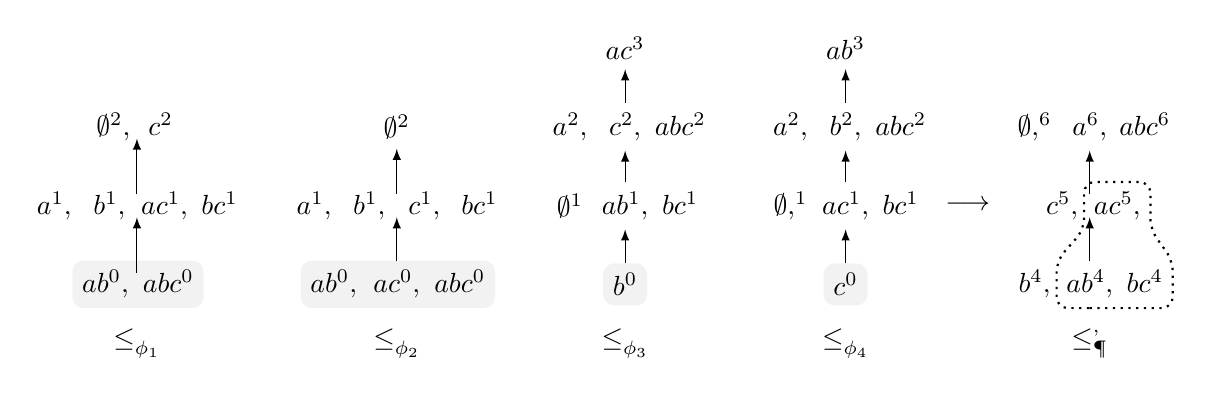
\begin{tikzpicture}
		%% phi1
		\node at (0,-0.75){$\le^{\hamming}_{\phi_1}$};

		\node at (-0.4,0)(ab){$ab^0,$};
		\node at (0.4,0)(abc){$abc^0\vphantom{,}$};
		\node[inner sep=0.4em] at (0,0)(a1){};
	
		\node at (-1.05,1)(a){$\vphantom{b,}a^1,$};	
		\node at (-0.35,1)(b){$b^1,$};		
		\node at (0.35,1)(ac){$\vphantom{b}ac^1,$};
		\node at (1.05,1)(bc){$bc^1\vphantom{,}$};
		\node[inner sep=0.4em] at (0,1)(a2){};

		\node at (-0.3,2)(e){$\emptyset^2,$};
		\node at (0.3,2)(c){$\vphantom{\emptyset,}c^2$};
		\node[inner sep=0.4em] at (0,2)(a3){};

		\path[-latex] (a1) edge (a2)(a2)edge(a3);
		
		\fill[opacity=0.05, rounded corners=4]
			(ab.south)--(abc.south)--(abc.south east)--(abc.east)--(abc.north east)--(abc.north)--
			(ab.north)--(ab.north west)--(ab.west)--(ab.south west)--(ab.south);


		%% phi2	
		\node at (3.3,-0.75){$\le^{\hamming}_{\phi_2}$};

		\node at (2.5,0)(ab){$ab^0,$};
		\node at (3.3,0)(ac){$ac^0,$};
		\node at (4.1,0)(abc){$abc^0\vphantom{,}$};
	
		\node at (2.25,1)(a){$\vphantom{b,}a^1,$};	
		\node at (2.95,1)(b){$b^1,$};		
		\node at (3.65,1)(c){$\vphantom{b}c^1,$};
		\node at (4.35,1)(bc){$bc^1\vphantom{,}$};
		\node[inner sep=0.4em] at (3.3,1)(a2){};

		\node at (3.3,2)(e){$\emptyset^2$};
		\node[inner sep=0.4em] at (0,2)(a3){};
	
		\path[-latex] (ac)edge(a2)(a2)edge(e);
		
		\fill[opacity=0.05, rounded corners=4]
			(ab.south)--(abc.south)--(abc.south east)--(abc.east)--(abc.north east)--(abc.north)--
			(ab.north)--(ab.north west)--(ab.west)--(ab.south west)--(ab.south);


		%% phi3	
		\node at (6.2,-0.75){$\le^{\hamming}_{\phi_3}$};

		\node at (6.2,0)(b){$b^0$};

		\node at (5.5,1)(e){$\emptyset^1$};
		\node at (6.2,1)(ab){$ab^1\vphantom{\emptyset},$};
		\node at (6.9,1)(bc){$bc^1\vphantom{\emptyset,}$};

		\node at (5.5,2)(a){$\vphantom{b,}a^2,$};	
		\node at (6.2,2)(c){$\vphantom{b}c^2,$};
		\node at (6.9,2)(abc){$abc^2\vphantom{,}$};

		\node at (6.2,3)(ac){$ac^3$};		
	
		\path[-latex] (b)edge(ab)(ab)edge(c)(c)edge(ac);

		\fill[opacity=0.05, rounded corners=4]
			(b.south)--(b.south east)--(b.east)--(b.north east)--(b.north)--
			(b.north west)--(b.west)--(b.south west)--(b.south);


		%% phi4
		\node at (9,-0.75){$\le^{\hamming}_{\phi_4}$};

		\node at (9,0)(c){$c^0$};

		\node at (8.3,1)(e){$\emptyset,^1$};
		\node at (9,1)(ac){$ac^1\vphantom{\emptyset},$};
		\node at (9.7,1)(bc){$bc^1\vphantom{\emptyset,}$};

		\node at (8.3,2)(a){$\vphantom{b}a^2,$};	
		\node at (9,2)(b){$b^2,$};
		\node at (9.7,2)(abc){$abc^2\vphantom{,}$};

		\node at (9,3)(ab){$ab^3$};		
	
		\path[-latex] (c)edge(ac)(ac)edge(b)(b)edge(ab);

		\fill[opacity=0.05, rounded corners=4]
			(c.south)--(c.south east)--(c.east)--(c.north east)--(c.north)--
			(c.north west)--(c.west)--(c.south west)--(c.south);

		%% arrow
		\node at (10.55,1.3){$\ssum$};
		\node at (10.55,1){$\longrightarrow$};


		%% sum result
		\node at (12.1,-0.75){$\le^{\hamming,\:\ssum}_{\P}$};

		\node at (11.4,0)(b){$b^4,$};
		\node at (12.1,0)(ab){$ab^4,$};
		\node at (12.8,0)(bc){$bc^4\vphantom{\emptyset,}$};

		\node at (11.75,1)(c){$c^5,$};		
		\node[inner sep=0.4em] at (12.1,1)(a2){};
		\node at (12.45,1)(ac){$ac^5\vphantom{\emptyset},$};

		\node at (11.4,2)(e){$\emptyset,^6$};
		\node at (12.1,2)(a){$\vphantom{\emptyset}a^6,$};	
		\node at (12.8,2)(abc){$abc^6\vphantom{,}$};

		\path[-latex] (ab)edge(a2)(a2)edge(a);

		\draw[thick, dotted, rounded corners=4]
			(ab.south)--(bc.south)--(bc.south east)--(bc.east)--(bc.north east)--
			(ac.south east)--(ac.east)--(ac.north east)--(ac.north)--(ac.north west)--
			(ac.west)--(ac.south west)--(ab.north west)--(ab.west)--(ab.south west)--(ab.south);
	\end{tikzpicture}
	\caption{
		Total preorders $\le^\hamming_{\phi_i}$, for $i\in\{1,2,3,4\}$, 
		corresponding to the opinions of the four Academy members in 
		Example \ref{ex:3-merging-distance-ops},
		as well as the aggregated preorder 
		$\le^{\hamming,\:\ssum}_{\P}$, 
		corresponding to the profile $\P$.
		The models of the result are the 
		most preferred models of the constraint $\mu$
		(depicted here in the area bordered by the dotted line) 
		in the collective preorder $\le_\P$.
		The superscripts next to each interpretation 
		stand for distances; the $\ssum$ aggregation function
		is written above the arrow separating the preorders in the profile
		from the collective preorder $\le^{\hamming,\:\ssum}_{\P}$.
	}
	\label{fig:3-merging-distance-ops}
\end{figure}


\begin{xmpl}{$\#$OscarsSoFossilized, with distances}{3-merging-distance-ops}
	For the setting in Example \ref{ex:3-merging-basic-setup},
	with $\Atoms=\{a,b,c\}$,
	the profile is $\P=(\phi_{1},\phi_{2}, \phi_{3}, \phi_{4})$,
	with
	$\phi_1 = a\land b$,
	$\phi_2 = a\land (b\lor c)$,
	$\phi_3 = \lnot a\land b \land \lnot c$.
	and
	$\phi_4 = \lnot a \land\lnot b\land c$.
	The constraint is $\mu$, 
	with
	$\mu=(a\land b\land \lnot c)\lor (a\land\lnot b\land c)\lor(\lnot a\land b\land c)$.
	The Hamming distances from formulas in the profile $\P$ to each interpretation $w$,
	together with the aggregated distances according to the $\leximax$, $\leximin$
	and $\ssum$ aggregation functions, 
	are depicted in Table \ref{tab:3-merging-hamming-distances}.
	The preorders $\le^{\hamming}_{\phi_{i}}$, as well as the aggregated preorder 
	$\le^{\hamming,\:\ssum}_{\P}$, are depicted in Figure \ref{fig:3-merging-distance-ops}.
	We obtain that:
	$$
		\dd_\hamming(\phi_1,ab)=\min(\dd_\hamming(ab,ab),\dd_\hamming(abc,ab))=\min(0,1)=0,
	$$
	and that:
	$$
		\dd^\ssum_\hamming(\P,ab) = \dd_{\hamming}(\phi_1,ab)+\dd_{\hamming}(\phi_2,ab)
		+\dd_{\hamming}(\phi_3,ab)+\dd_{\hamming}(\phi_4,ab) = 4.
	$$
	With the other aggregation functions, 
	we have that $\dd^\leximax_\hamming(\P,ab) = (3,1,0,0)$,
	i.e., the vector of distances from the formulas in $\P$ to $ab$ ordered in descending order,
	and $\dd^\leximin_\hamming(\P,ab) = (0,0,1,3)$,
	i.e., the vector of distances from the formulas in $\P$ to $ab$ ordered in ascending order.
	Note that 
	$ab \approx^{\hamming,\:\ssum}_{\P} bc$, since $\dd^\ssum_\hamming(\P,ab) = \dd^\ssum_\hamming(\P,bc)$.
	However, the situation is different when using the other aggregating functions:
	$bc <^{\hamming,\:\leximax}_{\P} ab$, since $(1,1,1,1)<_\lex(3,1,0,0)$,
	and $ab <^{\hamming,\:\leximin}_{\P} bc$, since $(0,0,1,3)<_\lex(1,1,1,1)$.
	We obtain that 
	$[\me^{\hamming,\:\leximax}_\mu(\P)]=\{bc\}$,
	$[\me^{\hamming,\:\leximin}_\mu(\P)]=\{ab\}$
	and
	$[\me^{\hamming,\:\ssum}_\mu(\P)]=\{ab,bc\}$.
\end{xmpl}

The operators 
$\me^{\hamming,\:\ssum}$,
$\me^{\hamming,\:\leximax}$
and 
$\me^{\hamming,\:\leximin}$
all embody different attitudes to the aggregation of information.
Intuitively, 
$\me^{\hamming,\:\ssum}$ sees optimal outcomes in utilitarian terms and thereby favors the majority opinion, 
while $\me^{\hamming,\:\leximax}$ attempts to improve the situation of the worse off agent, and usually veers towards egalitarian outcomes;
the $\me^{\hamming,\:\leximin}$ operator is elitist, in that it favors outcomes that improve the situation of the best off agent.
On the other hand, the operators 
$\me^{\drastic,\:\ssum}$, 
$\me^{\drastic,\:\leximax}$
and
$\me^{\drastic,\:\leximin}$,
on the other hand, are all equivalent, i.e., 
$\me^{\drastic,\:\ssum}_\mu(\P)\equiv\me^{\drastic,\:\leximin}_\mu(\P)\equiv\me^{\drastic,\:\leximax}_\mu(\P)$,
for any propositional profile $\P$ and formula $\mu$. 

The difference between majoritarian and egalitarian operators can be hashed out in 
terms of the following postulates \cite{LiberatoreS98,KoniecznyP11}, 
to be thought of in conjunction with postulates $\ppm{0-8}$
and applying for any $\L$-profiles $\P_1$ and $\P_2$,
constraints $\mu$, $\mu_1$ and $\mu_2$, and formulas $\phi_1$ and $\phi_2$:

\begin{description}
	\item[($\ppm{\MAJ}$)] There exists an integer $n$ such that 
		$\me_{\mu}(\P_1+(\underbrace{\P_2+\dots+\P_2}_{n~\text{times}}))\models \me_{\mu}(\P_2)$. 
	\item[($\ppm{\ARB}$)] If $\me_{\mu_1}(\phi_1)\equiv \me_{\mu_2}(\P_2)$,
		$\me_{\mu_1\leftrightarrow\lnot\mu_2}(\phi_1,\phi_2)\equiv \mu_1\leftrightarrow\lnot\mu_2$,
		$\mu_1\not\models\mu_2$ and $\mu_2\not\models\mu_1$,
		then $\me_{\mu_1\lor\mu_2}(\phi_1,\phi_2)\equiv \me_{\mu_1}(\phi_1)$.
\end{description}

Postulate $\ppm{\MAJ}$ says that a large enough coalition 
will sway the merging result in its favor,
while postulate $\ppm{\ARB}$ formalizes the idea that 
the median position is to be preferred \cite{LiberatoreS98}.
We will not delve too much into these properties, 
except to say that operators $\me^{\dd,\:\ssum}$ satisfy postulate $\ppm{\MAJ}$
and operators $\me^{\dd,\:\leximax}$ satisfy postulate $\ppm{\ARB}$.































\section{Related work}\label{sec:3-rw}
Belief change in the sense relevant to us here 
begins, in earnest, with the AGM model of the $1980$s
\cite{AlchourronGM85,AlchourronM85,Gardenfors88},
with some of the main ideas going back,
according to Peter G\"ardenfors \cite{Gardenfors11},
slightly further \cite{Harper76,Levi80}. 

The original AGM publications led to a watershed of works attempting 
to model belief change operators, and revision in particular, in 
more intuitive terms. Important proposals used 
entrenchment relations \cite{GardenforsM88},
systems of spheres \cite{Grove88}
and preorders on possible worlds \cite{KatsunoM92}.
All of these models rely, in some way or another, on 
preferences, either among formulas or interpretations.
The latter reference, of course, provides the basis for our own work,
with a closely related model \cite{KatsunoM91} providing the basis 
for our presentation of update.
It should be mentioned that the AGM model assumes a language 
that subsumes propositional logic, and, as such, is strictly more general 
than the Katsuno-Mendelzon model taken here as reference point. 
Nonetheless, the choice mechanisms that underly revision 
are similar across all representations:
we chose the Katsuno-Mendelzon model 
because, in our opinion, it exhibits these mechanisms in a way that is
intuitive and that lends itself to applications across various other domains.

In the initial AGM model revision was often placed side by side 
with \emph{contraction}, deemed equally important and analysed as a belief 
change operation in its own right. 
Contraction models removals of certain items of knowledge from a bigger corpus:
in the terminology used here, contraction of $\phi$ with respect to $\mu$
would require changing $\phi$ in such a way that $\mu$ is not implied by the result.
Though we have not looked at it here, contraction also
affords an interpretation in terms of choice over interpretations \cite{CaridroitKM17}.
In most formal models contraction and revision are intended to be
inter-definable, with a sizeable literature devoted to finding solutions 
for when they are not \cite{Delgrande08,DelgrandeW10,DelgrandeW13,ZhuangPZ13,ZhuangPZ17}.

Belief revision was understood early on to have many ideas in common
with rational choice \cite{Doyle91,Rott93,Schulte99}, with Hans Rott's book \cite{Rott01}
providing an in-depth analysis of these connections, together with a set of 
bold philosophical claims. Most of the claims presented in Section \ref{sec:3-revision}
can be traced, in some way or another, to this work. Nonetheless, the formal model 
we work with is different, and the results, when not following directly 
from the Katsuno-Mendelzon paper \cite{KatsunoM92}, were derived from scratch.
There are more recent takes on the parallel between revision and rational choice 
\cite{Bonanno09,Arlo-CostaP10,Hansson14}, but our impression is that the Katsuno-Mendelzon model
remains the easiest one to work with. That postulates $\ppr{1}$, $\ppr{3}$ and $\ppr{5-6}$
are essentially the same as the axioms for choice functions circulating in the 
literature on rational choice is, thus, news to no one, and it has even been argued that 
the equivalence is not a coincidence \cite{Olsson03}.

Even Hans Rott's book, in all its comprehenesiveness, only looks at 
single-agent operations, which, in rational choice terms, is 
equivalent to individual decision makers. 
This is undoubtedly because at the time when Hans Rott was writing his book
the framework for merging \cite{LiberatoreS98,KoniecznyP02,KoniecznyM04,KoniecznyP11}
had not yet been fully developed.
As is clear by now, our view is that merging is to revision as social choice 
is to individual rational choice. There is nothing new about this either,
with several publications attempting to build bridges between merging 
and social choice \cite{Meyer01,MeyerGC01,KoniecznyP05,EckertP05,EveraereKM07,EveraereKM14,DiazP17,EveraereKM17}.

Our work on enforcement came out of an attempt to axiomatize enforcement in
abstract argumentation \cite{Baumann12,WallnerNJ17}, but the postulates took on 
a life of their own when formulated in propositional logic. 
The same postulates, we discovered later, had been used to model the dynamics of \emph{desire} 
\cite{DuboisLP17}, though the duality with revision embodied in Equations 
\ref{eq:revision-to-enforcement} and \ref{eq:enforcement-to-revision} had not been explicitly stated.
Since enforcement does not guarantee full acceptance of the new information $\mu$, 
it shares a similarity with \emph{non-prioritized revision} \cite{Hansson99b,HanssonFCF01}
and \emph{belief promotion} operators \cite{SchwindKM18}.
However, since the postulates characterizing enforcement, and in particular, 
its success postulate $\ppe{2}$, are different, enforcement does not coincide 
with any of the proposals in this literature.

A useful comparison can be made with contraction, 
overlooked in this work but which is, as mentioned above,
an important member of the belief change family.
Contraction of a propositional formula $\phi$ by a 
propositional formula $\mu$ can be represented as a choice 
function using the identity $[\phi]\cup\min_{\le_{\phi}}[\lnot\mu]$,
where $\le_{\phi}$ is a familiar, r-faithful preorder on interpretations that 
depends on $\phi$ \cite{CaridroitKM17}. In other words,
the models of the contraction are obtained by adding 
the most plausible models of $\lnot\mu$, according to $\le_{\phi}$,
to the models of $\phi$.
Consider, now, the following example.

\begin{xmpl}{Enforcement vs contraction}{3-enforcement-vs-contraction}
	For a set of atoms $\Atoms=\{a,b\}$, 
	take $[\phi] = \{a\}$ and $[\mu]=\{b\}$. 
	Then the result of enforcing $\mu$
	with respect to $\phi$ is $[\phi\en\mu]=\phi\lor\mu=\{a,b\}$,
	if the enforcement operator $\en$ satisfies postulate $\ppe{2}$.
	On the other hand, contracting $\phi$ with respect to $\mu$ results 
	in the set of interpretations: 
	\begin{align*}
		[\phi]\cup\min_{\le_{\phi}}[\lnot\mu] &= \{a\}\cup\min_{\le_{\phi}}\{\emptyset,a,ab\}\\ 
											  &= \{a\}\cup\{a\}\\ 
											  & = \{a\}.
	\end{align*}
	The latter equality holds because $\le_{\phi}$ is assumed to satisfy the properties 
	of an r-faithful assignment, such that $\min_{\le_{\phi}}\{\emptyset,a,ab\} = \{a\}$.

	Thus, an agent who starts off believing that $a$ is the true state of the world 
	and queries a source that advocates for $b$
	will want to use an enforcement operator if the source is deemed credible enough.
	If, on the other hand, the source is deemed untrustowrthy and the agent wants to remove 
	any information stemming from it, then it will use an contraction operator.
\end{xmpl}

Note that the result of contraction
in Example \ref{ex:3-enforcement-vs-contraction} is the same 
regardless of the particular preorder $\le_{\phi}$ used,
as long as $\le_{\phi}$ satisfies the properties of an r-faithful assignment.
Thus, Example \ref{ex:3-enforcement-vs-contraction} trades on what are uncontroversial 
cases for both enforcement and contraction, i.e., cases in which the result 
is unambiguously determined on the basis of the standard postulates alone.
As such, it highlights the differences in how incoming information is treated 
by the two operations.







\section{Conclusion}\label{sec:3-conclusion} 
This chapter has introduced us 
to the main vehicles of belief change
we will be studying throughout the rest of this work:
revision, update, enforcement and merging.
The defining characteristics of a belief change operator,
we have seen, are the logical postulates used to axiomatize it,
the preferences over outcomes that items of prior information 
are assumed to influence,
and the optimization behavior shown,
through various representation theorems,
to characterize belief change operators.

One of the aims of this chapter has been to show
that belief change operations can be understood
as choice procedures over the space of interpretations.
The poster child for this approach is revision, 
which presents itself as a straightforward analogue
to choice functions studied in rational choice theory
\cite{Sen69,Sen70,GrantvZ09}.
Theorem \ref{thm:3-revision-repr-total}, in particular, 
tells us that an agent revising beliefs $\phi$ along the lines of
postulates $\ppr{1}$ and $\ppr{3-6}$ 
behaves as if it ranks outcomes
in a total preorder $\le_{\phi}$,
and always picks the minimal models of 
of the new information $\mu$ according to $\le_{\phi}$.
Such an agent, then, behaves like a rational agent
choosing the best elements from a given menu of options:
the menu, here, consists of the models of $\mu$, i.e., 
the possible worlds the agent is allowed to believe
in light of new information,
while the best elements are decided with reference to $\le_{\phi}$.
% Thus, a revision operator can be readily seen as a \emph{choice function}
% over sets of interpretations:
Revision postulates $\ppr{1}$ and $\ppr{3}$
are equivalent to properties $\ooch{1}$ and $\ooch{2}$
of a choice function, 
as presented in 
Section \ref{sec:2-choice-functions},
while postulates $\ppr{5}$ and $\ppr{6}$
are roughly equivalent to 
or properties $\ooch{3}$ and $\ooch{4}$, 
or properties $\alpha$ and $\beta$, 
as they are known in the theory of rational choice \cite{Sen69,Sen70}.
Postulate $\ppr{4}$, though it does not have 
an analogue in rational choice theory,
reinforces the parallel by making sure that revision operators
are not sensitive to the syntax of the formulas involved.
Thus, taken together, postulates $\ppr{1}$ and $\ppr{3-6}$ 
characterize choice functions over outcomes 
rationalizable by total preorders:
accordingly, Theorem \ref{thm:3-revision-repr-total} aligns
with standard choice theoretic results \cite{Arrow51,Sen69}.
The main difference 
between rational choice and revision, then, 
lies in the interpretation given to the concepts at play:
a preference order, in rational choice, 
ranks items in terms of their desirability,
whereas in belief change it ranks outcomes in terms of 
their plausibility.

In the wake of this result, we were able to make sense of other 
aspects of belief change through the lens of choice theory.
Theorem \ref{thm:3-revision-repr-partial}
showed that the optimization behavior 
in Theorem \ref{thm:3-revision-repr-total}
can be reproduced just as well with partial orders
instead of total orders.
Theorems \ref{thm:3-update-repr-km-total} and 
\ref{thm:3-update-repr-km-partial} showed that 
update fits nicely into this perspective,
with the choice being distributed across 
preorders induced by every model of 
the prior information $\phi$ 
rather than, as with revision, 
by $\phi$ as a whole.
Section \ref{sec:3-enforcement} introduced us 
to the novel type of belief change we called 
\emph{enforcement},
with Theorem \ref{thm:3-enforcement-repr} showing 
that choice in the case of enforcement assumes a
particular form: an enforcement operator has to 
figure out what models to add to the new information 
$\mu$, rather than what models to discard.
This is choice over outcomes that are not consistent 
with the new information, but choice nonetheless.
Finally, Theorem \ref{thm:3-merging-repr} showed us that 
the choice perspective lends itself naturally to 
belief merging operators, as they can be seen 
as collective choice procedures.

In recasting belief change operators as choice procedures,
postulate $\ppr{2}$, as well as its various incarnations,
i.e., postulates $\ppu{2}$, $\ppe{2}$ or $\ppm{2}$,
has been consistently put aside for separate treatment: 
this is because a belief change operator does not need it 
in order to function as a choice procedure.
As Theorems \ref{thm:3-revision-repr-R2-total}
and \ref{thm:3-revision-repr-R2-partial} show,
what postulate $\ppr{2}$, together with its avatars,
does is to bias the choice relative to $\phi$,
by making sure that models of $\phi$ are given 
priority in the choice process.
This is consistent with a view in which outcomes 
consistent with a belief $\phi$ are considered the 
most plausible states of affairs,
but raises the question as to what other attitudes 
towards these outcomes are reasonable.
This is a question we will tackle in the next chapter.

